%************************************************
\chapter{Research and Development For Future LXe TPCs}

\label{ch:RandD} % $\mathbb{ZNR}$
%************************************************

A small test bed was built at Lawrence Berkeley National Laboratory to study various detector effects facing large \ac{LXe} \ac{TPC}s. The test bed was built and instrumented over the course of about two years, from 2015 through 2016. This chapter describes some of the details of that instrumentation.

\section{Experimental Vessel}
The experimental vessel is a 

\section{Charge Amplifiers}
The segmented anode was instrumented with three CR-100 charge amplifiers from Cremat (Figure~\ref{fig:cr110}). The raw charge amplifier signals were each fed into a CR-160-R7 shaper evaluation board, also from Cremat. The evaluation board houses two more modules: one CR-200-X shaping amplifier and one CR-100 baseline restorer. The CR-200-X shaping amplifier is an X-$\mu$s gaussian shaping amplifier; it was determined that 1~$\mu$s was most appropriate for the test bed signals.

\begin{figure}[htbp]
\begin{center}
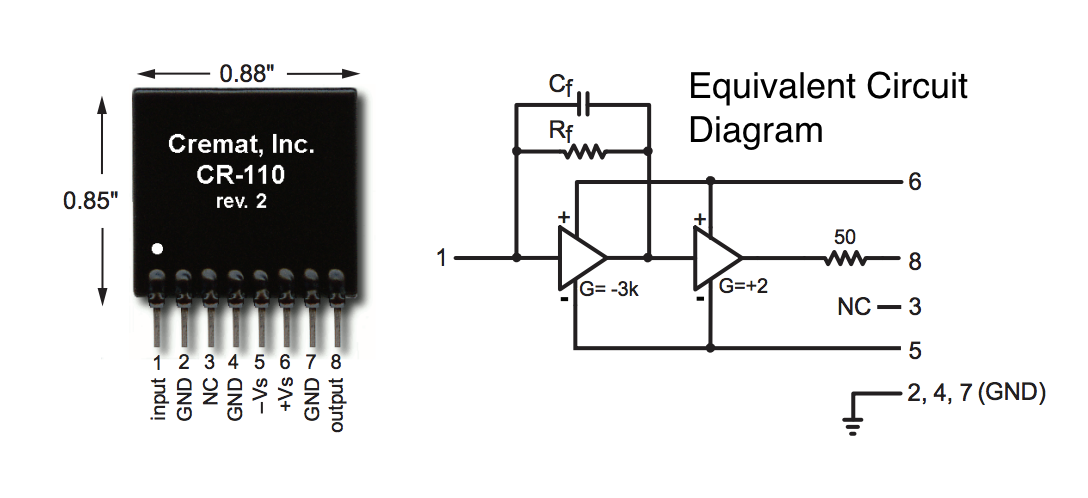
\includegraphics[width=4in]{figures/testbed/cr110.png}
\caption{A picture from the manufacturer's data sheet, shown with an equivalent circuit diagram.}
\label{fig:cr110}
\end{center}
\end{figure}

The shaper evaluation board produced gaussian pulses from raw charge signals as shown in Figure~\ref{fig:shaper}.

\begin{figure}[htbp]
\begin{center}
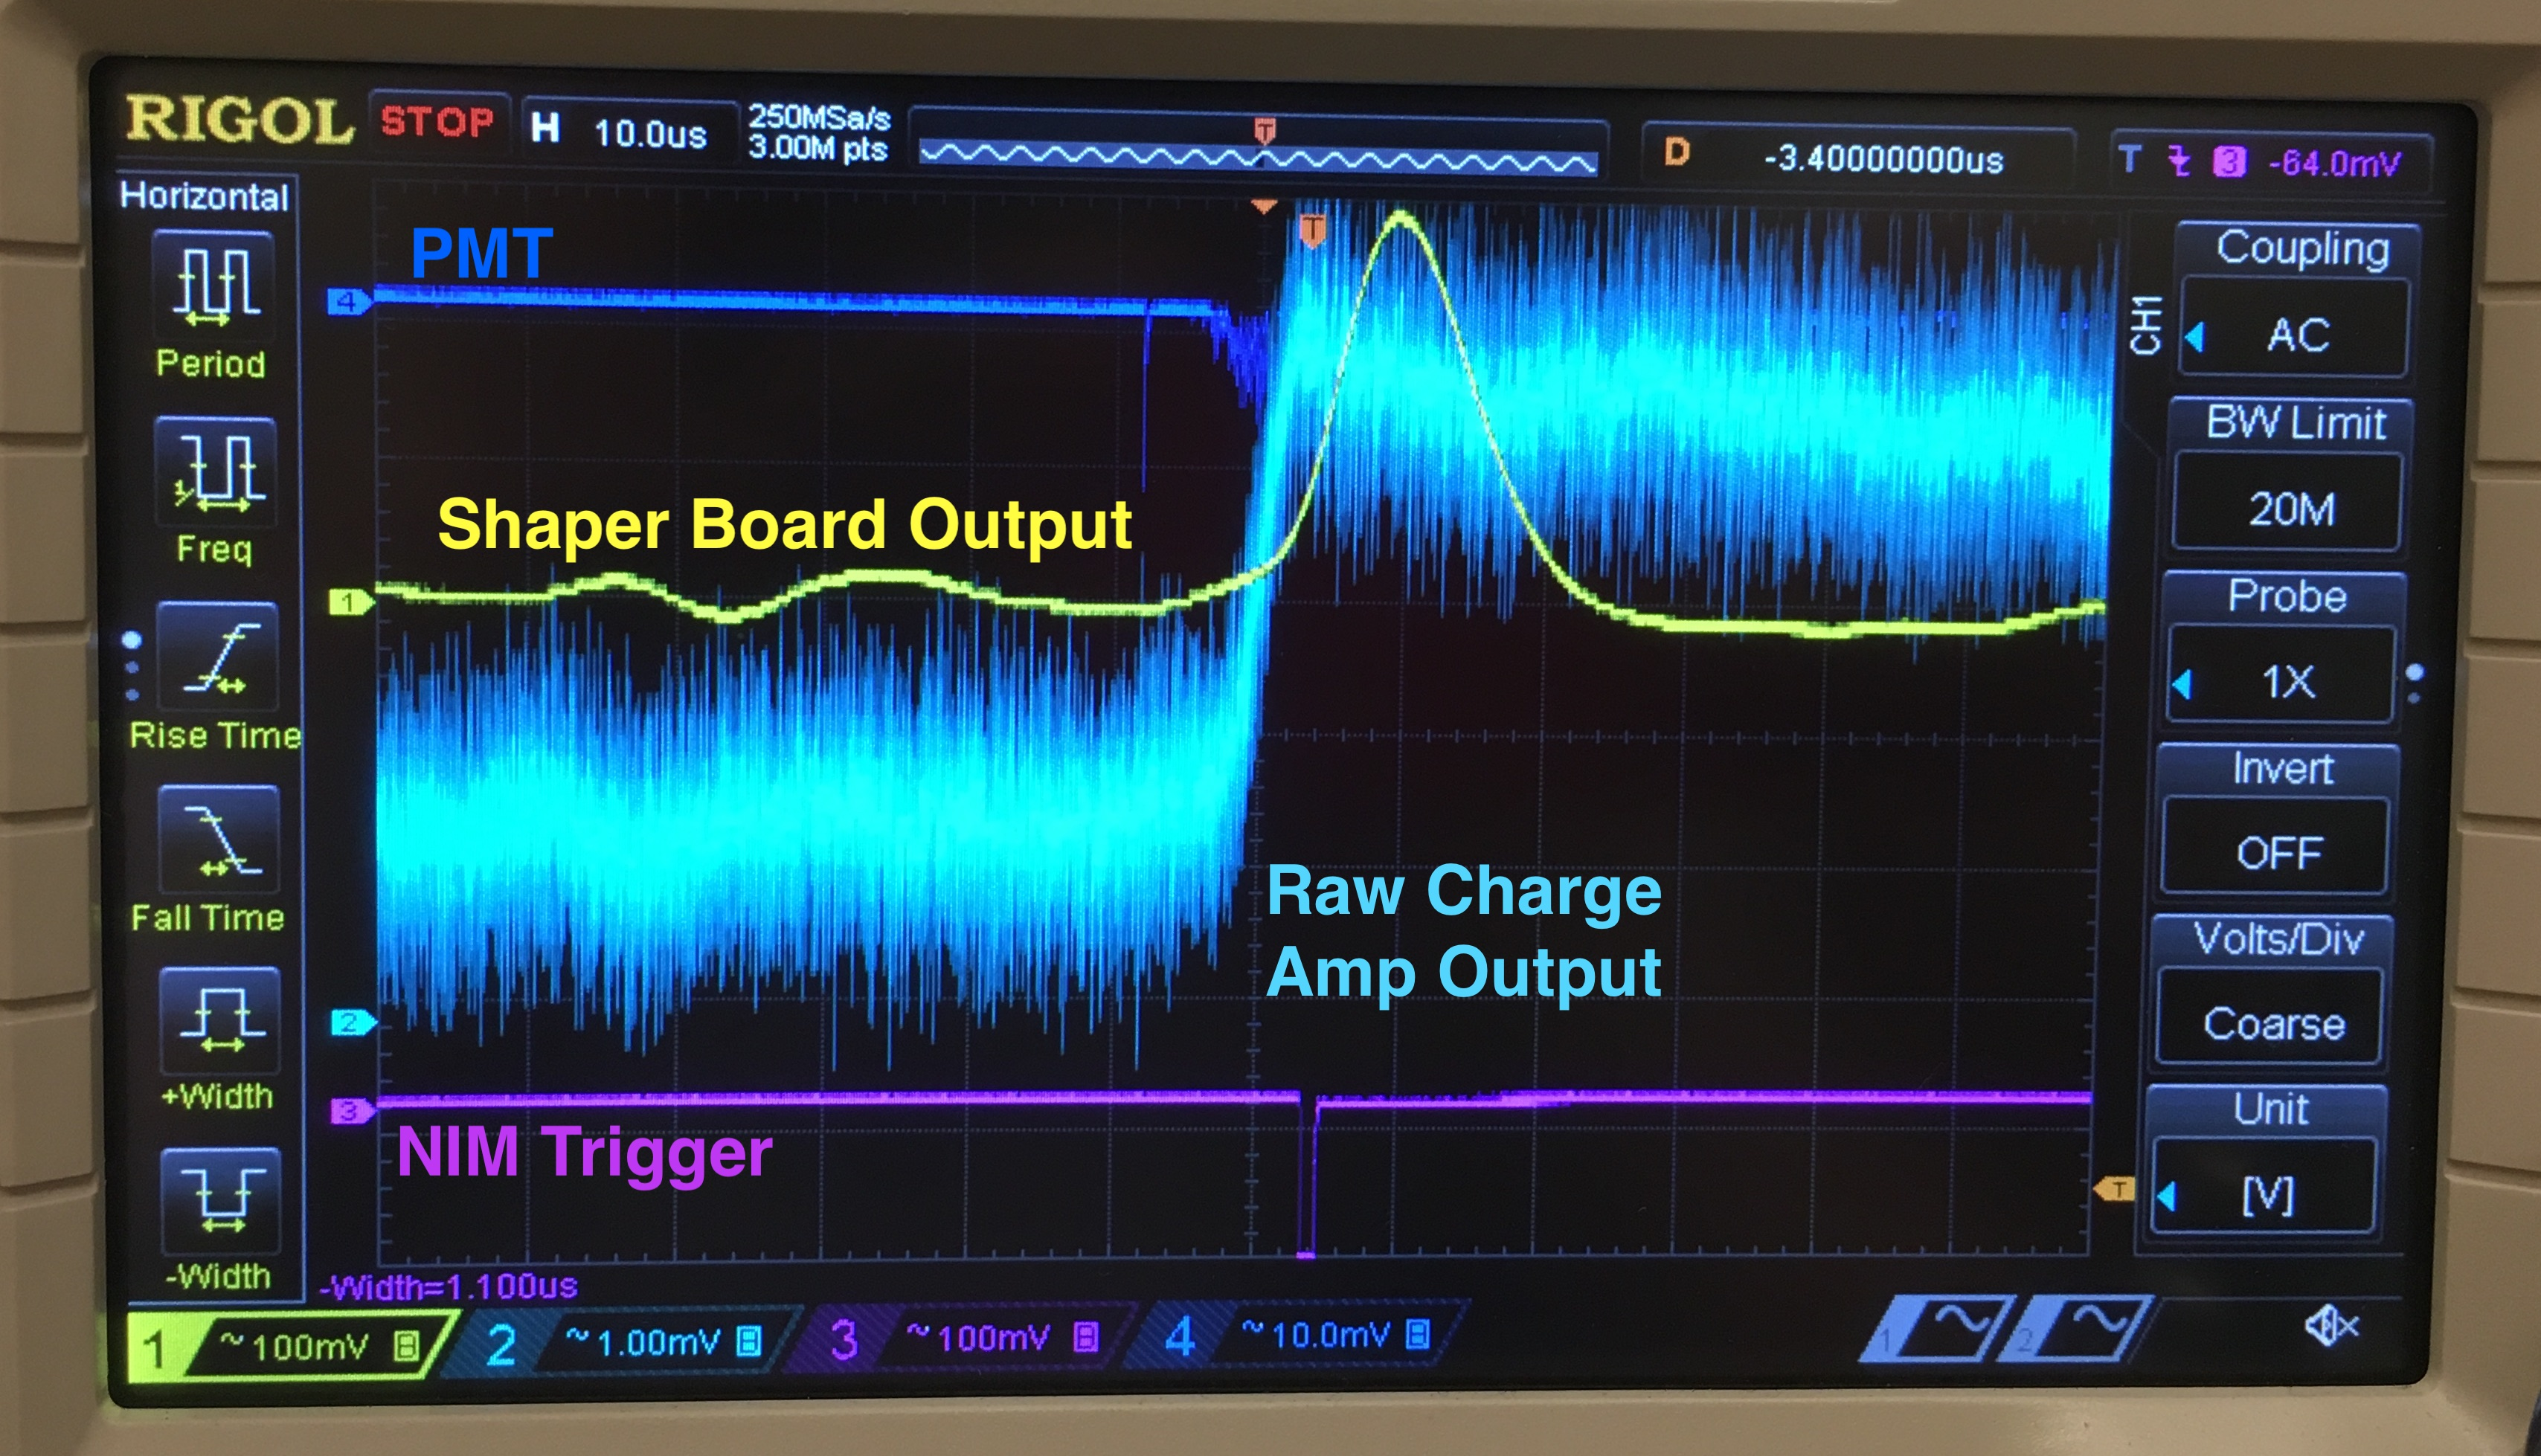
\includegraphics[width=4in]{figures/testbed/charge_amp_shaper.jpg}
\caption{A raw and shaped charge amp signal taken in -100C gaseous xenon, with the radon source plumed in}
\label{fig:shaper}
\end{center}
\end{figure}

The charge amplifiers were originally placed inside the experimental vessel, mounted directly on the segmented anode. The functionality at \ac{LXe} temperatures didn't deviate from manufacturer's specifications, however it was found that the CR-100 units generated enough heat to create a perpetual gas layer under the anode. In general this is not an issue, but for the purpose of the intended absolute electron extraction efficiency measurement, `overfilling' the TPC and using the charge amplifiers as a direct read-out of electrons in the liquid was required. The charge amplifiers were moved to the outer vessel space, surrounded by small Faraday cage made of copper mesh. See Figure~\ref{fig:chargeamp_mount} for the charge amplifier mounting configurations.

 \begin{figure}[htbp]
\begin{center}
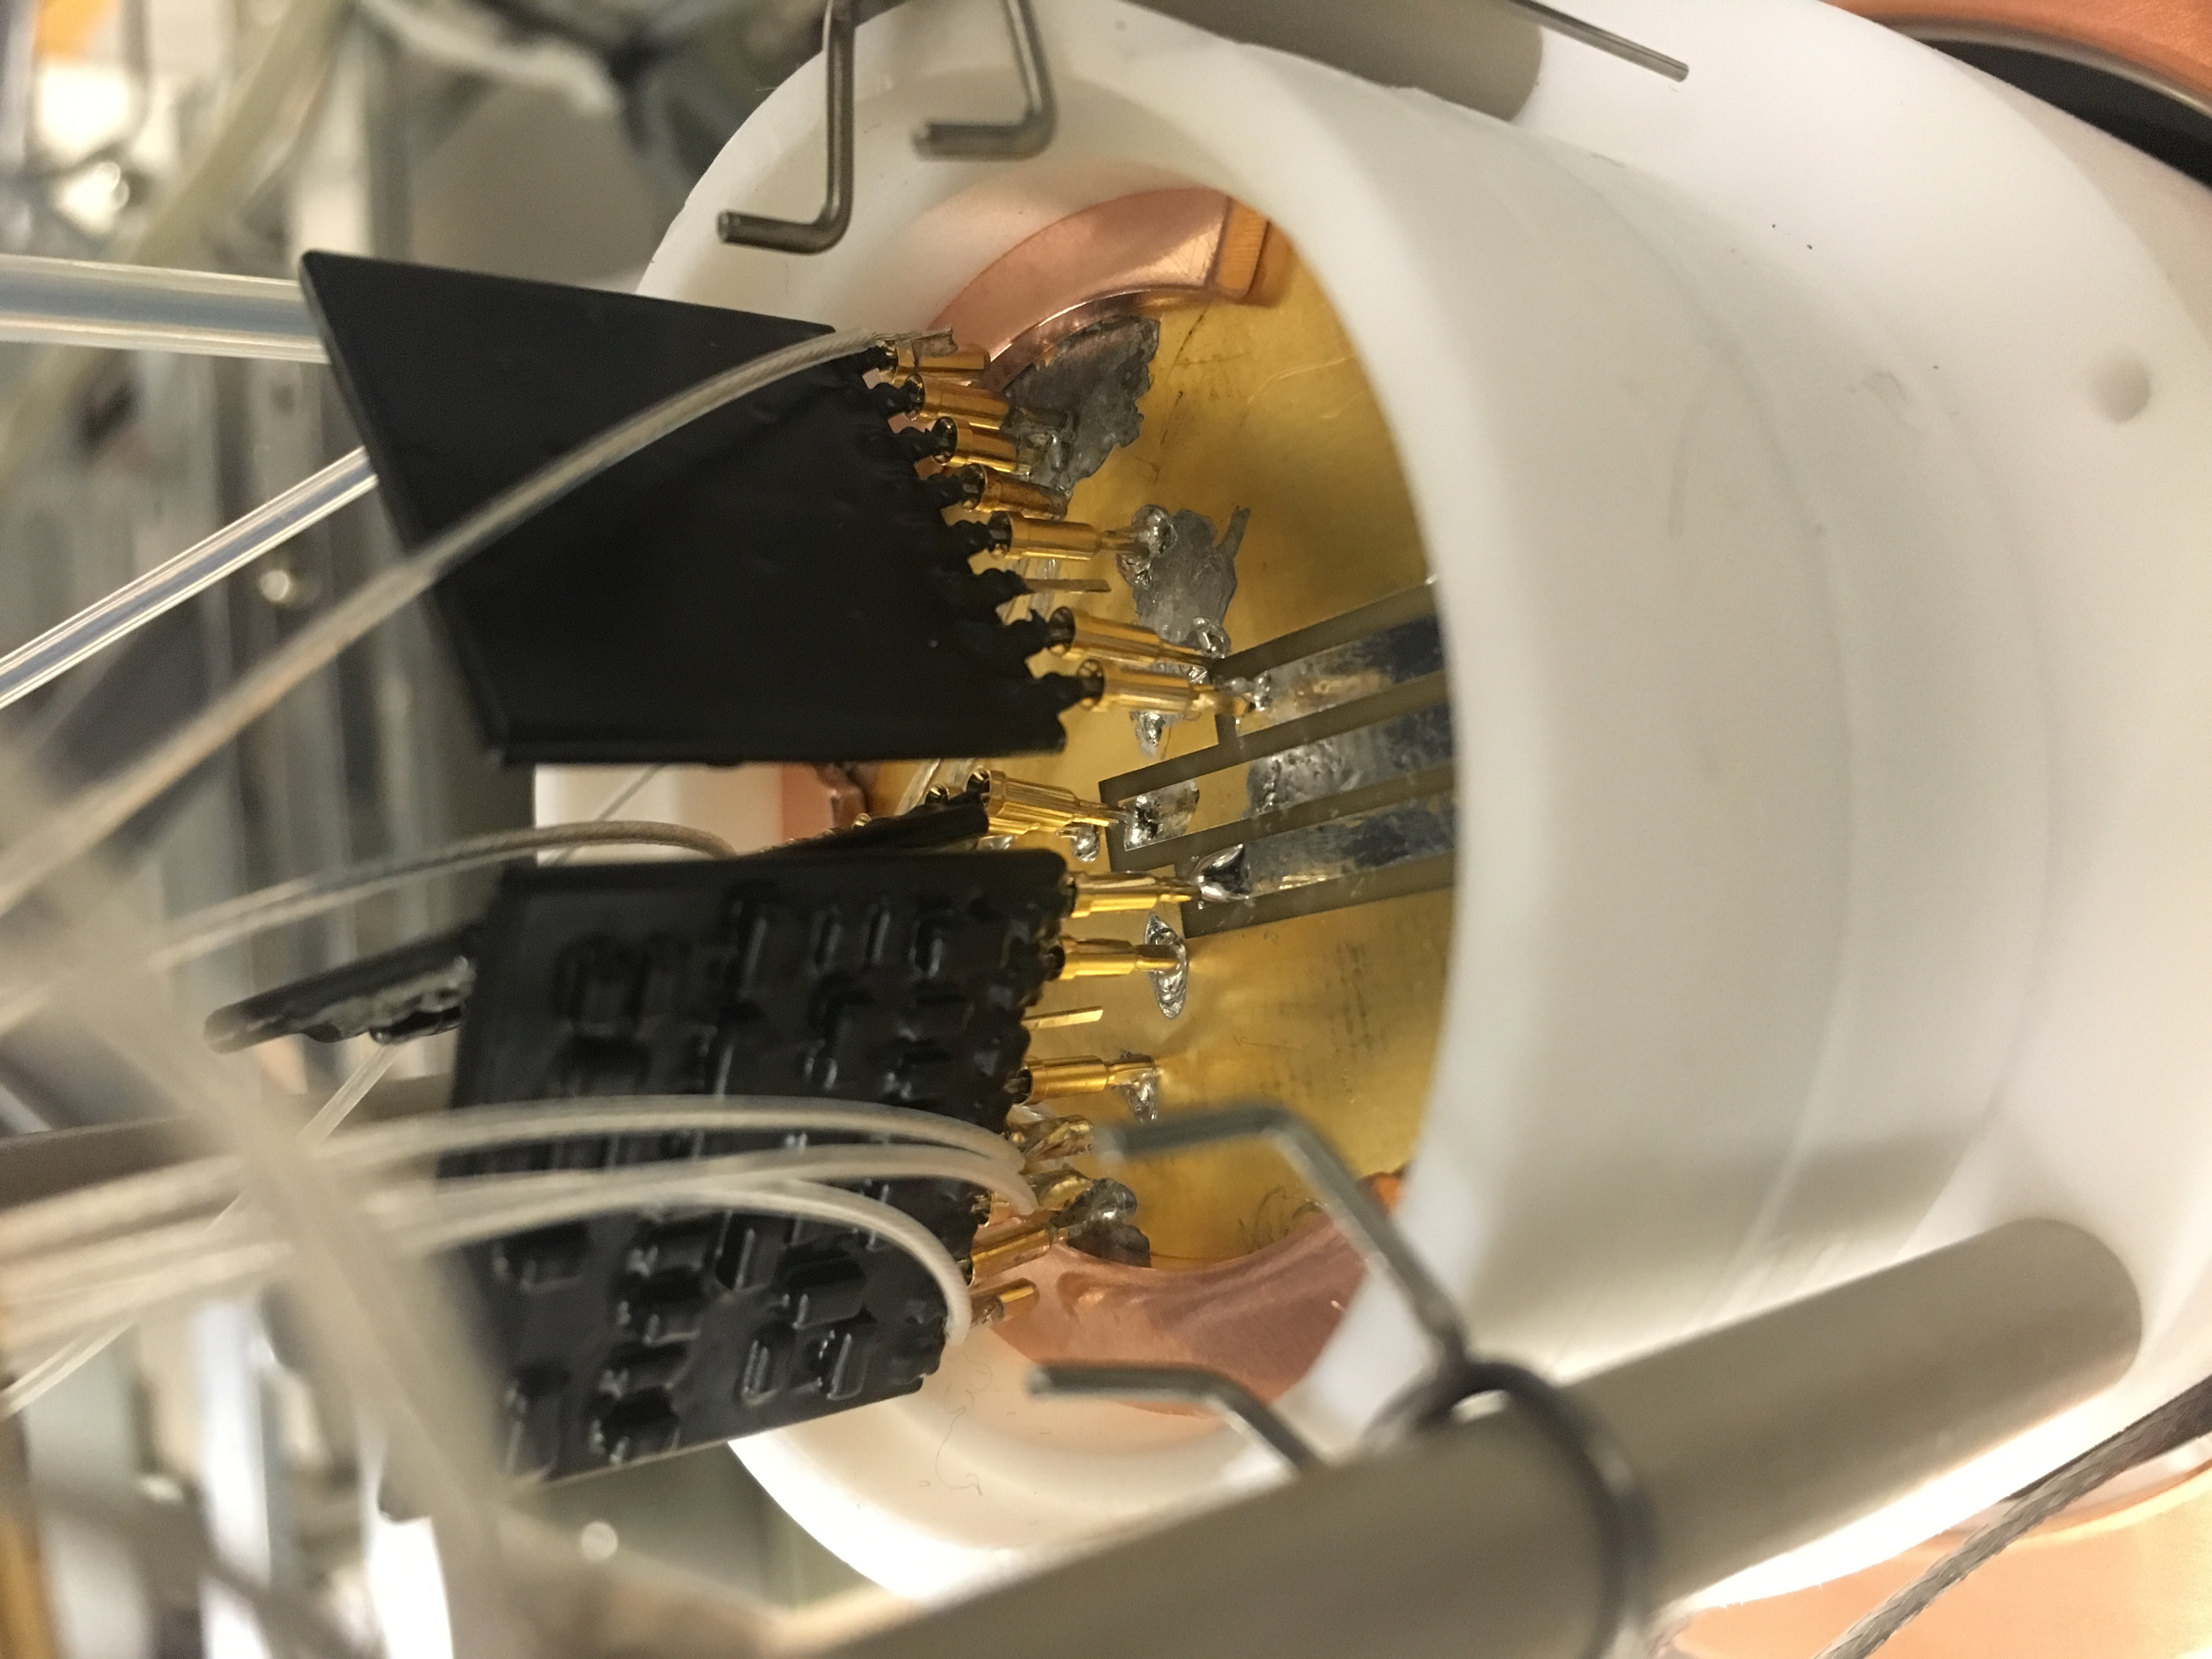
\includegraphics[width=\halffig]{figures/testbed/chargeamp_mount1.jpg}
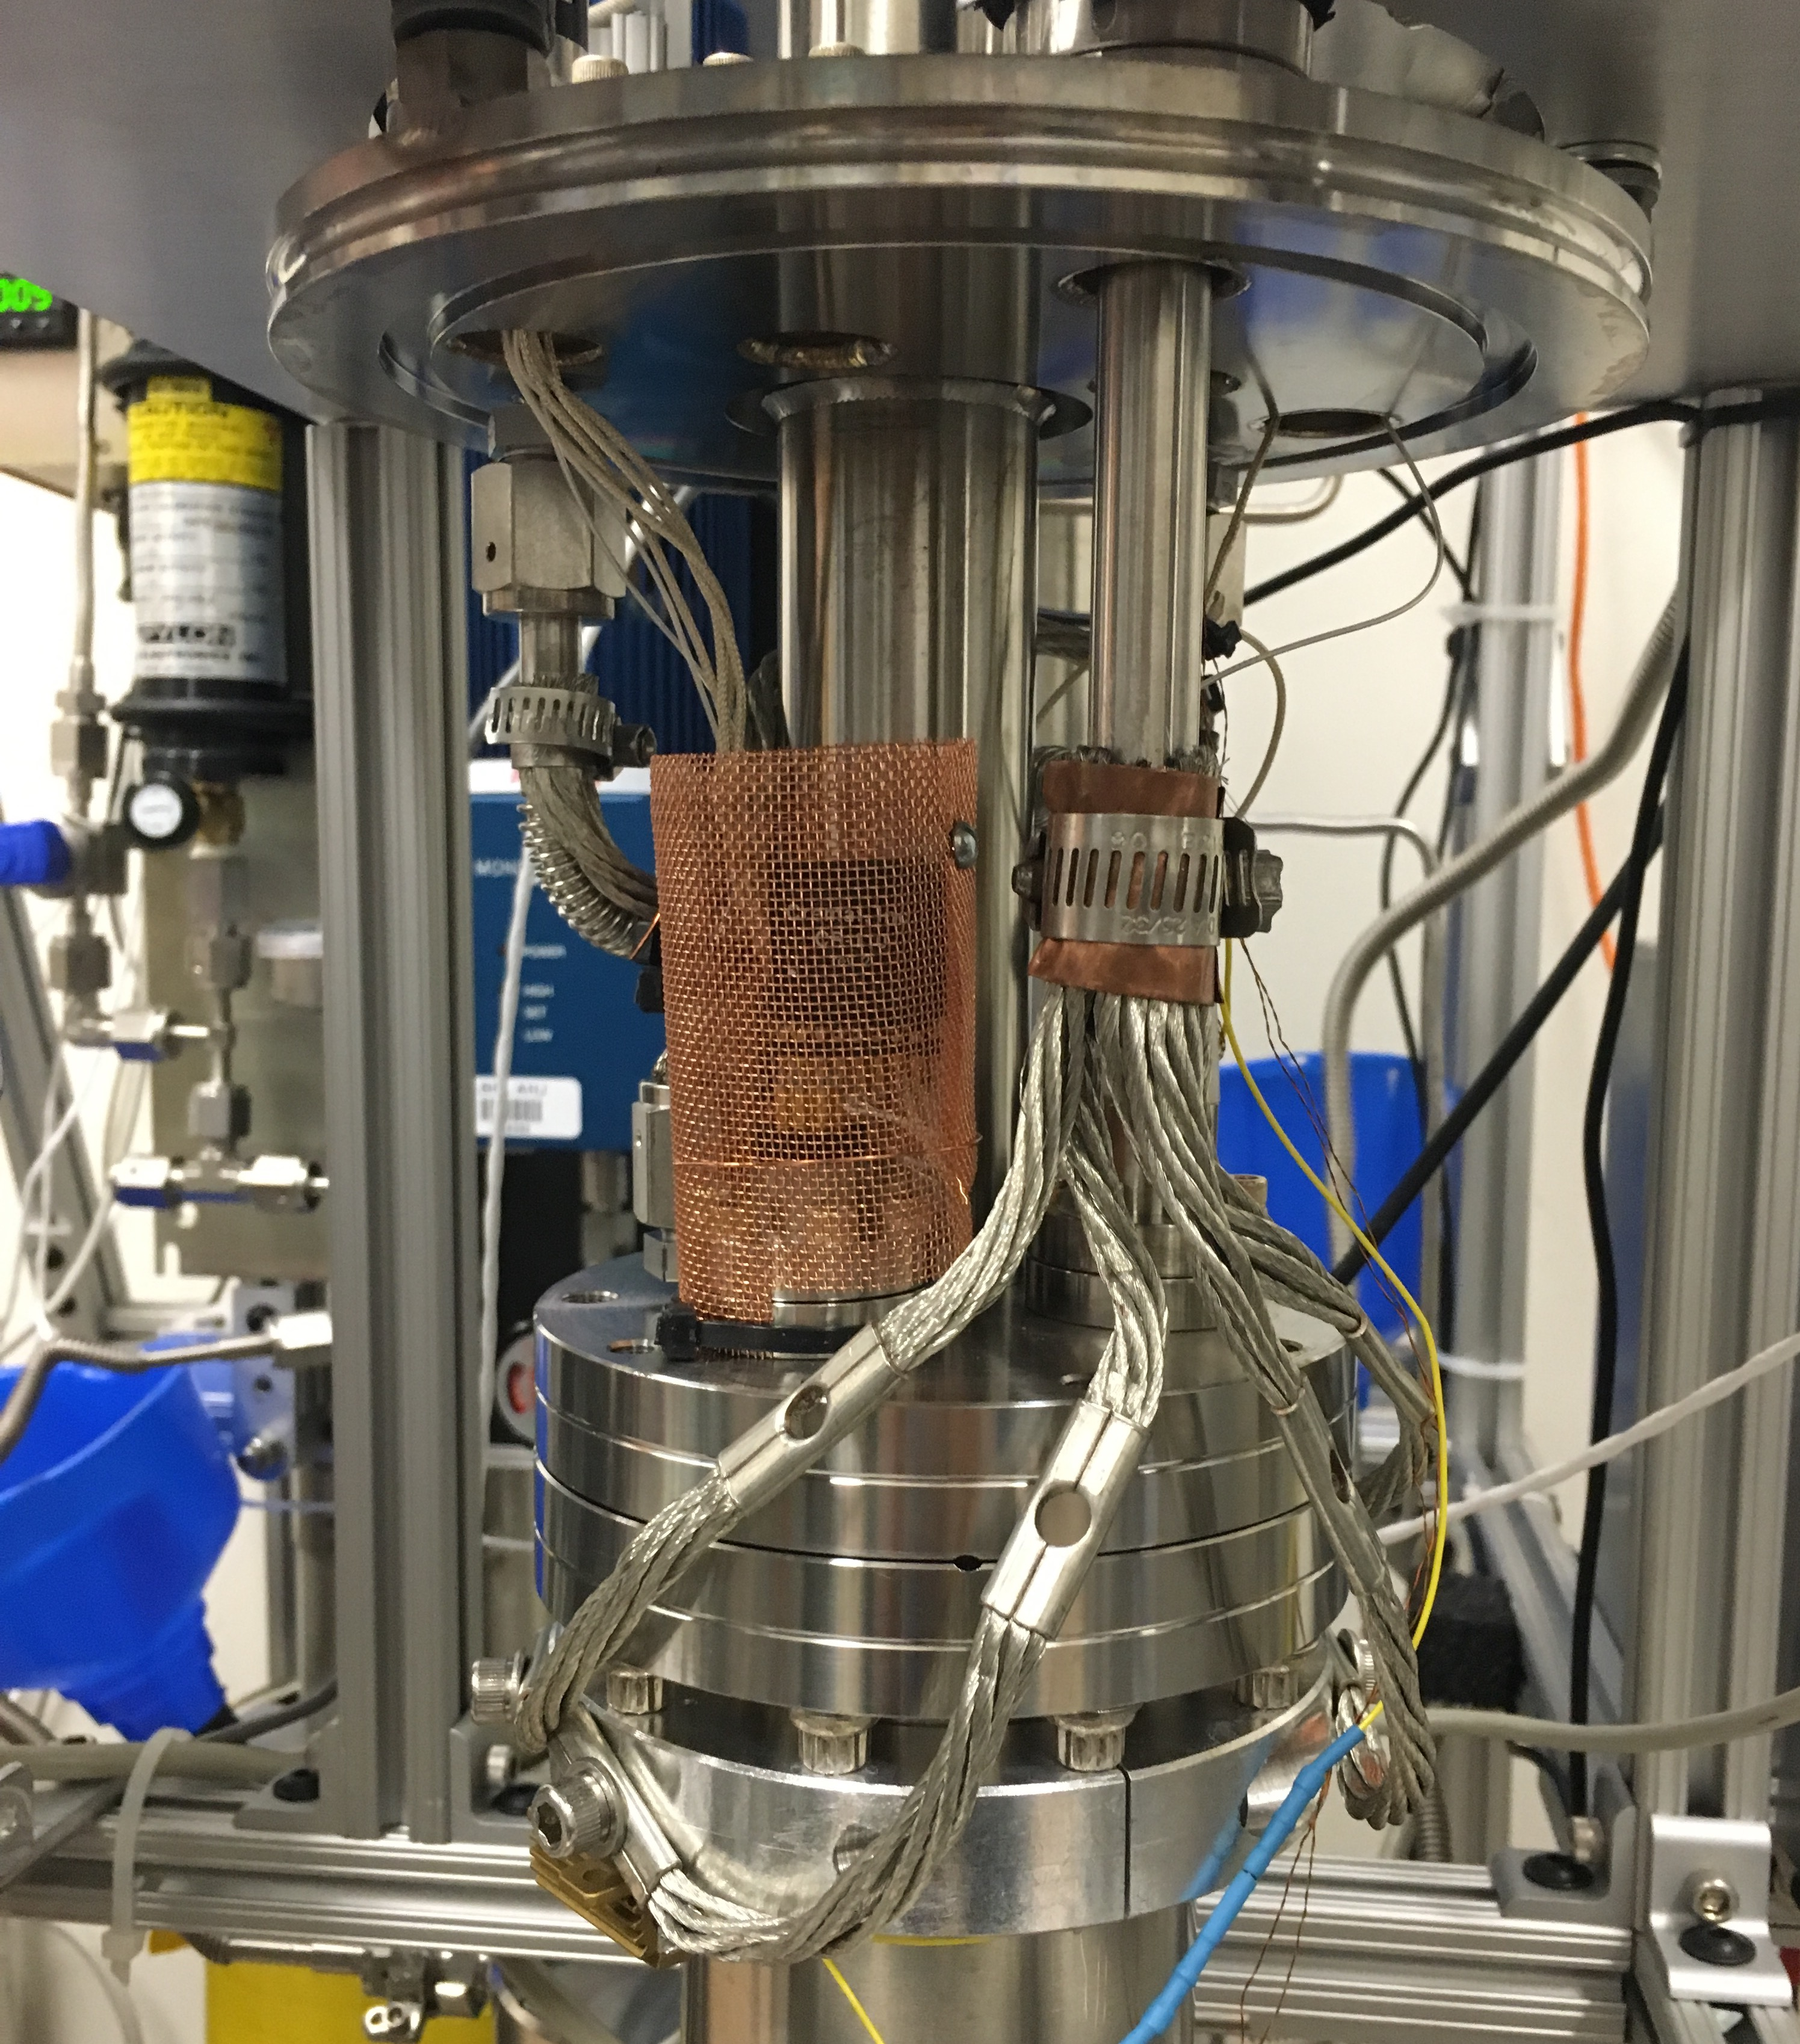
\includegraphics[width=\halffig]{figures/testbed/chargeamp_mount2.jpg}
\caption{(Right) original mounting of CR-110 charge amplifiers inside the experimental vessel. (Left) Mounting in the outer vacuum reduced head load on the TPC.}
\label{fig:chargeamp_mount}
\end{center}
\end{figure}



\section{PMT}
The test bed was instrumented with an R8778 PMT, the same PMTs used in LUX. Both LUX and LZ PMT bases were used. The radon daughters study presented in Chapter~\ref{ch:radon} exclusively used the LUX PMT base, the electron trains studies first used the LUX base, and later used the LZ base. The LZ base was favored for its larger capacitors. Various shaping amplifiers were used when digitizing the PMT over the course of these studies because the 8~ns sampling interval of the data acquisition was subject to aliasing the fast-rising alpha S1 signals.

%\subsection{PMT Saturation}

\section{Slow Control}

\section{Data Acquisition}
Data were acquired with a Picoscope 5000a, a USB-compatible ``oscilloscope." The picoscope python library was used to write voltage records of PMT and charge signals to ROOT files, which were opened later for reprocessing into reduced quantities such as pulse area or pulse height. The picoscope functioned as a 14~bit ADC with 125~MHz sampling. For special cases, when only one channel was desired, it was possible to increase the sampling rate to 500~MHZ (or 2~ns)



\section{High Voltage Feedthrough Design}
A significant amount of time was spent developing and testing \ac{HV} feedthroughs for the test bed. This section describes a few of the feedthroughs that were unsuccessful, leading to the final design, which is capable of delivering -11kV to the cathode with no observable breakdown or other effects. Extensive detail of the tests and procedures are not provided. Instead, the following vignettes are intended as an overview to be useful to a student tasked with designing a HV feedthrough. 

\subsection{Implementing SHV Feed Throughs from Vacuum Suppliers}
The first attempts at building feedthroughs were to use off-the-shelf products from typical vacuum supply vendors such as MDC and Kurt Lesker. Vacuum \ac{HV} feedthroughs are intended to for use from air to vacuum, not air to \ac{LXe}, so it is not surprising that these were not successful. Additionally, by combining ceramic and metal (typically aluminum, stainless steel, nickel, copper) they are especially prone to breakdown at the meeting of these different materials, known colloquially as ``triple points''. When there are interfaces between materials with different permittivities (dielectric constants), the electric fields are distorted.  Field is pushed out of the higher dielectric material into the lower dielectric material. This creates a field enhancement where peak fields can be much higher than average fields in the system. The field enhancement from "triple points" where there is in interface between a conductor and two dielectrics (e.g a plastic or ceramic feedthrough insulator and a gas or liquid) is a common source of breakdown along insulator surfaces. Good design practices, namely choices of geometry reduce the field enhancements in these regions.


Note that ceramic feedthroughs are not appropriate for low background experiments due to high radioactivity, but for test beds, where low radioactivity is not a priority, they may be used.

The first few feed throughs used a 12kV \ac{SHV} weldable feed though as shown in Figure~\ref{fig:12kV-SHV}. If used as operation is intended, the side indicated by A is used on the vacuum-side and B connects to the voltage supply. Instead, we trimmed the long B side and attached a copper, screw-port connector to make the 90 degree connection from vertical feed through to horizontal grid. This was done to avoid placing a conducting surface at high voltage (the tip of side A) in gaseous xenon, thereby increasing the risk of breakdown to the walls of the detector. The feed through's vertical placement is designed such that the copper connector is fully submersed in \ac{LXe}.

 
\begin{figure}[htbp]
\begin{center}
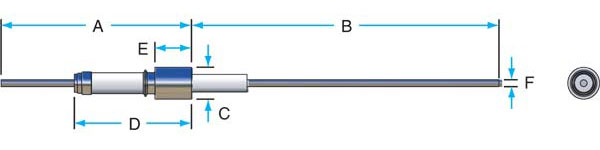
\includegraphics[width=5in]{figures/testbed/12kV-SHV.jpg}
\caption{A 12kV SHV weldable connector from vacuum supplier Kurt Lesker.}
\label{fig:12kV-SHV}
\end{center}
\end{figure}

\begin{figure}[htbp]
\begin{center}
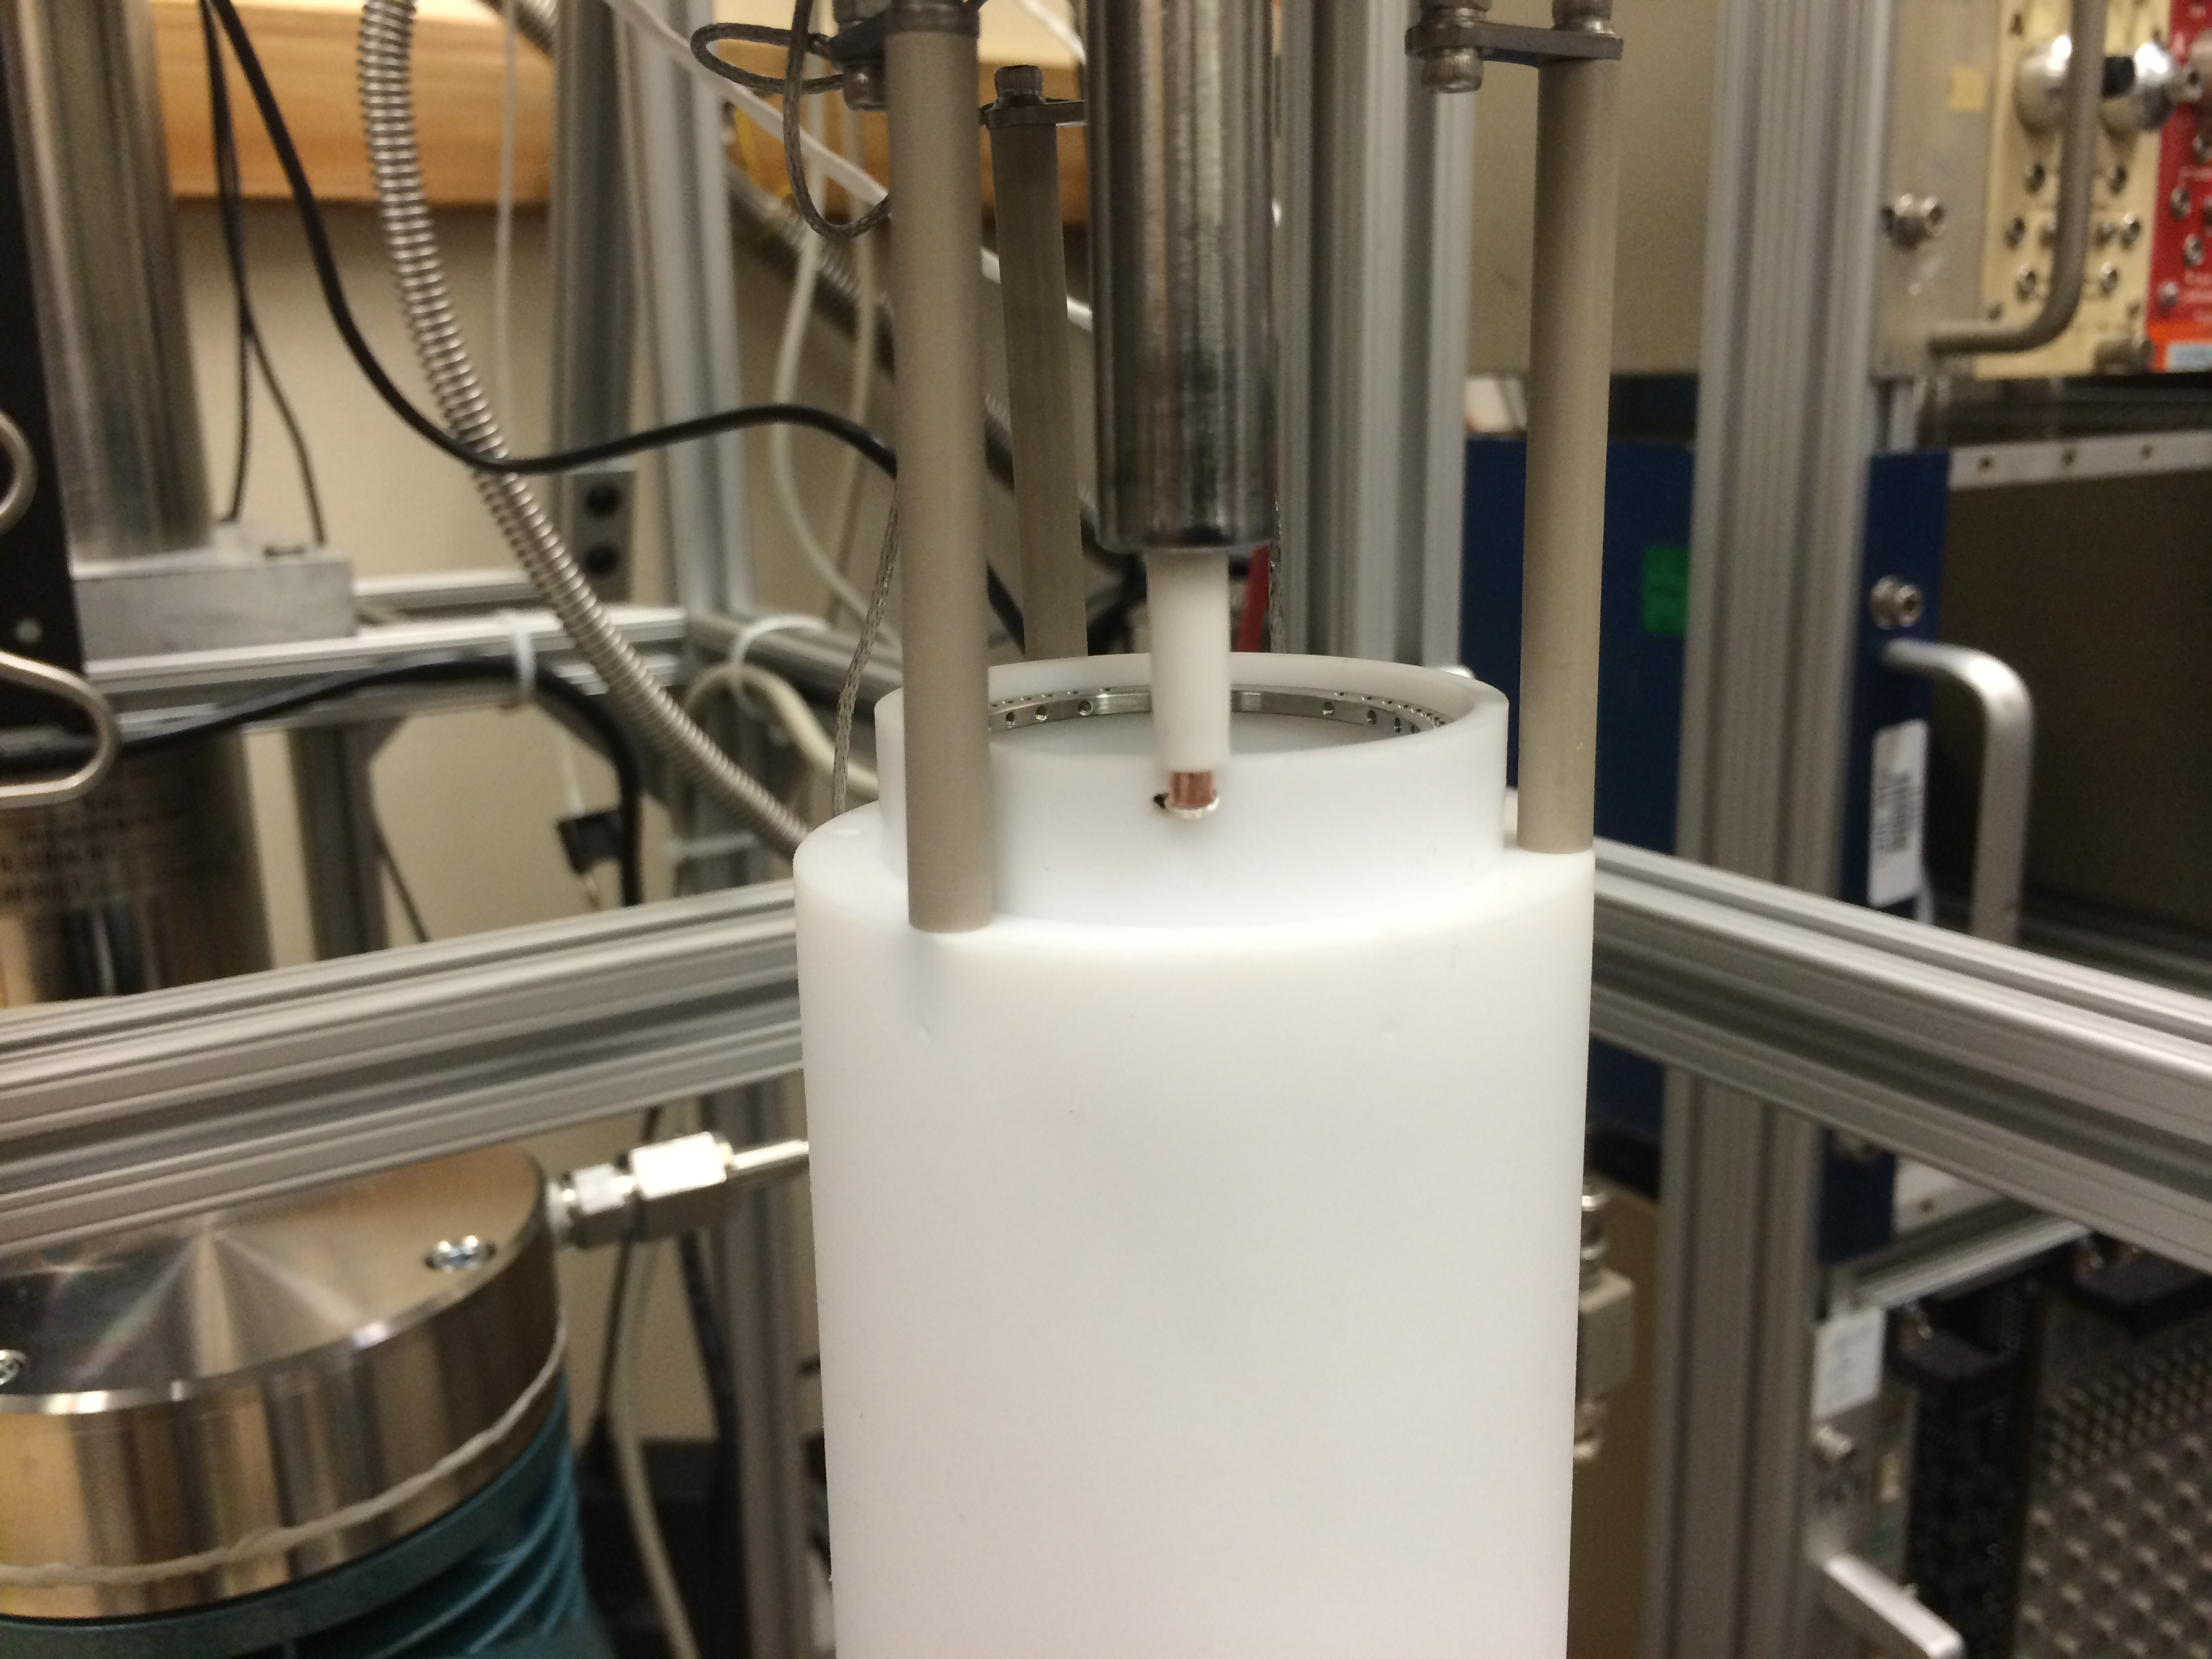
\includegraphics[width=3in]{figures/testbed/ft1_1.jpg}
\caption{12kV SHV weldable connector, inverted, clipped, and attached with a machined copper connector. The connector uses a screw to capture the SHV feed though, and the same screw to capture a stranded wire, visible in this picture, which is then fed through a hole drilled in the PTFE to connect to the wire grid frames. The wire was wrapped around the grid frame.}
\label{fig:ft1_1}
\end{center}
\end{figure}

\begin{figure}[htbp]
\begin{center}
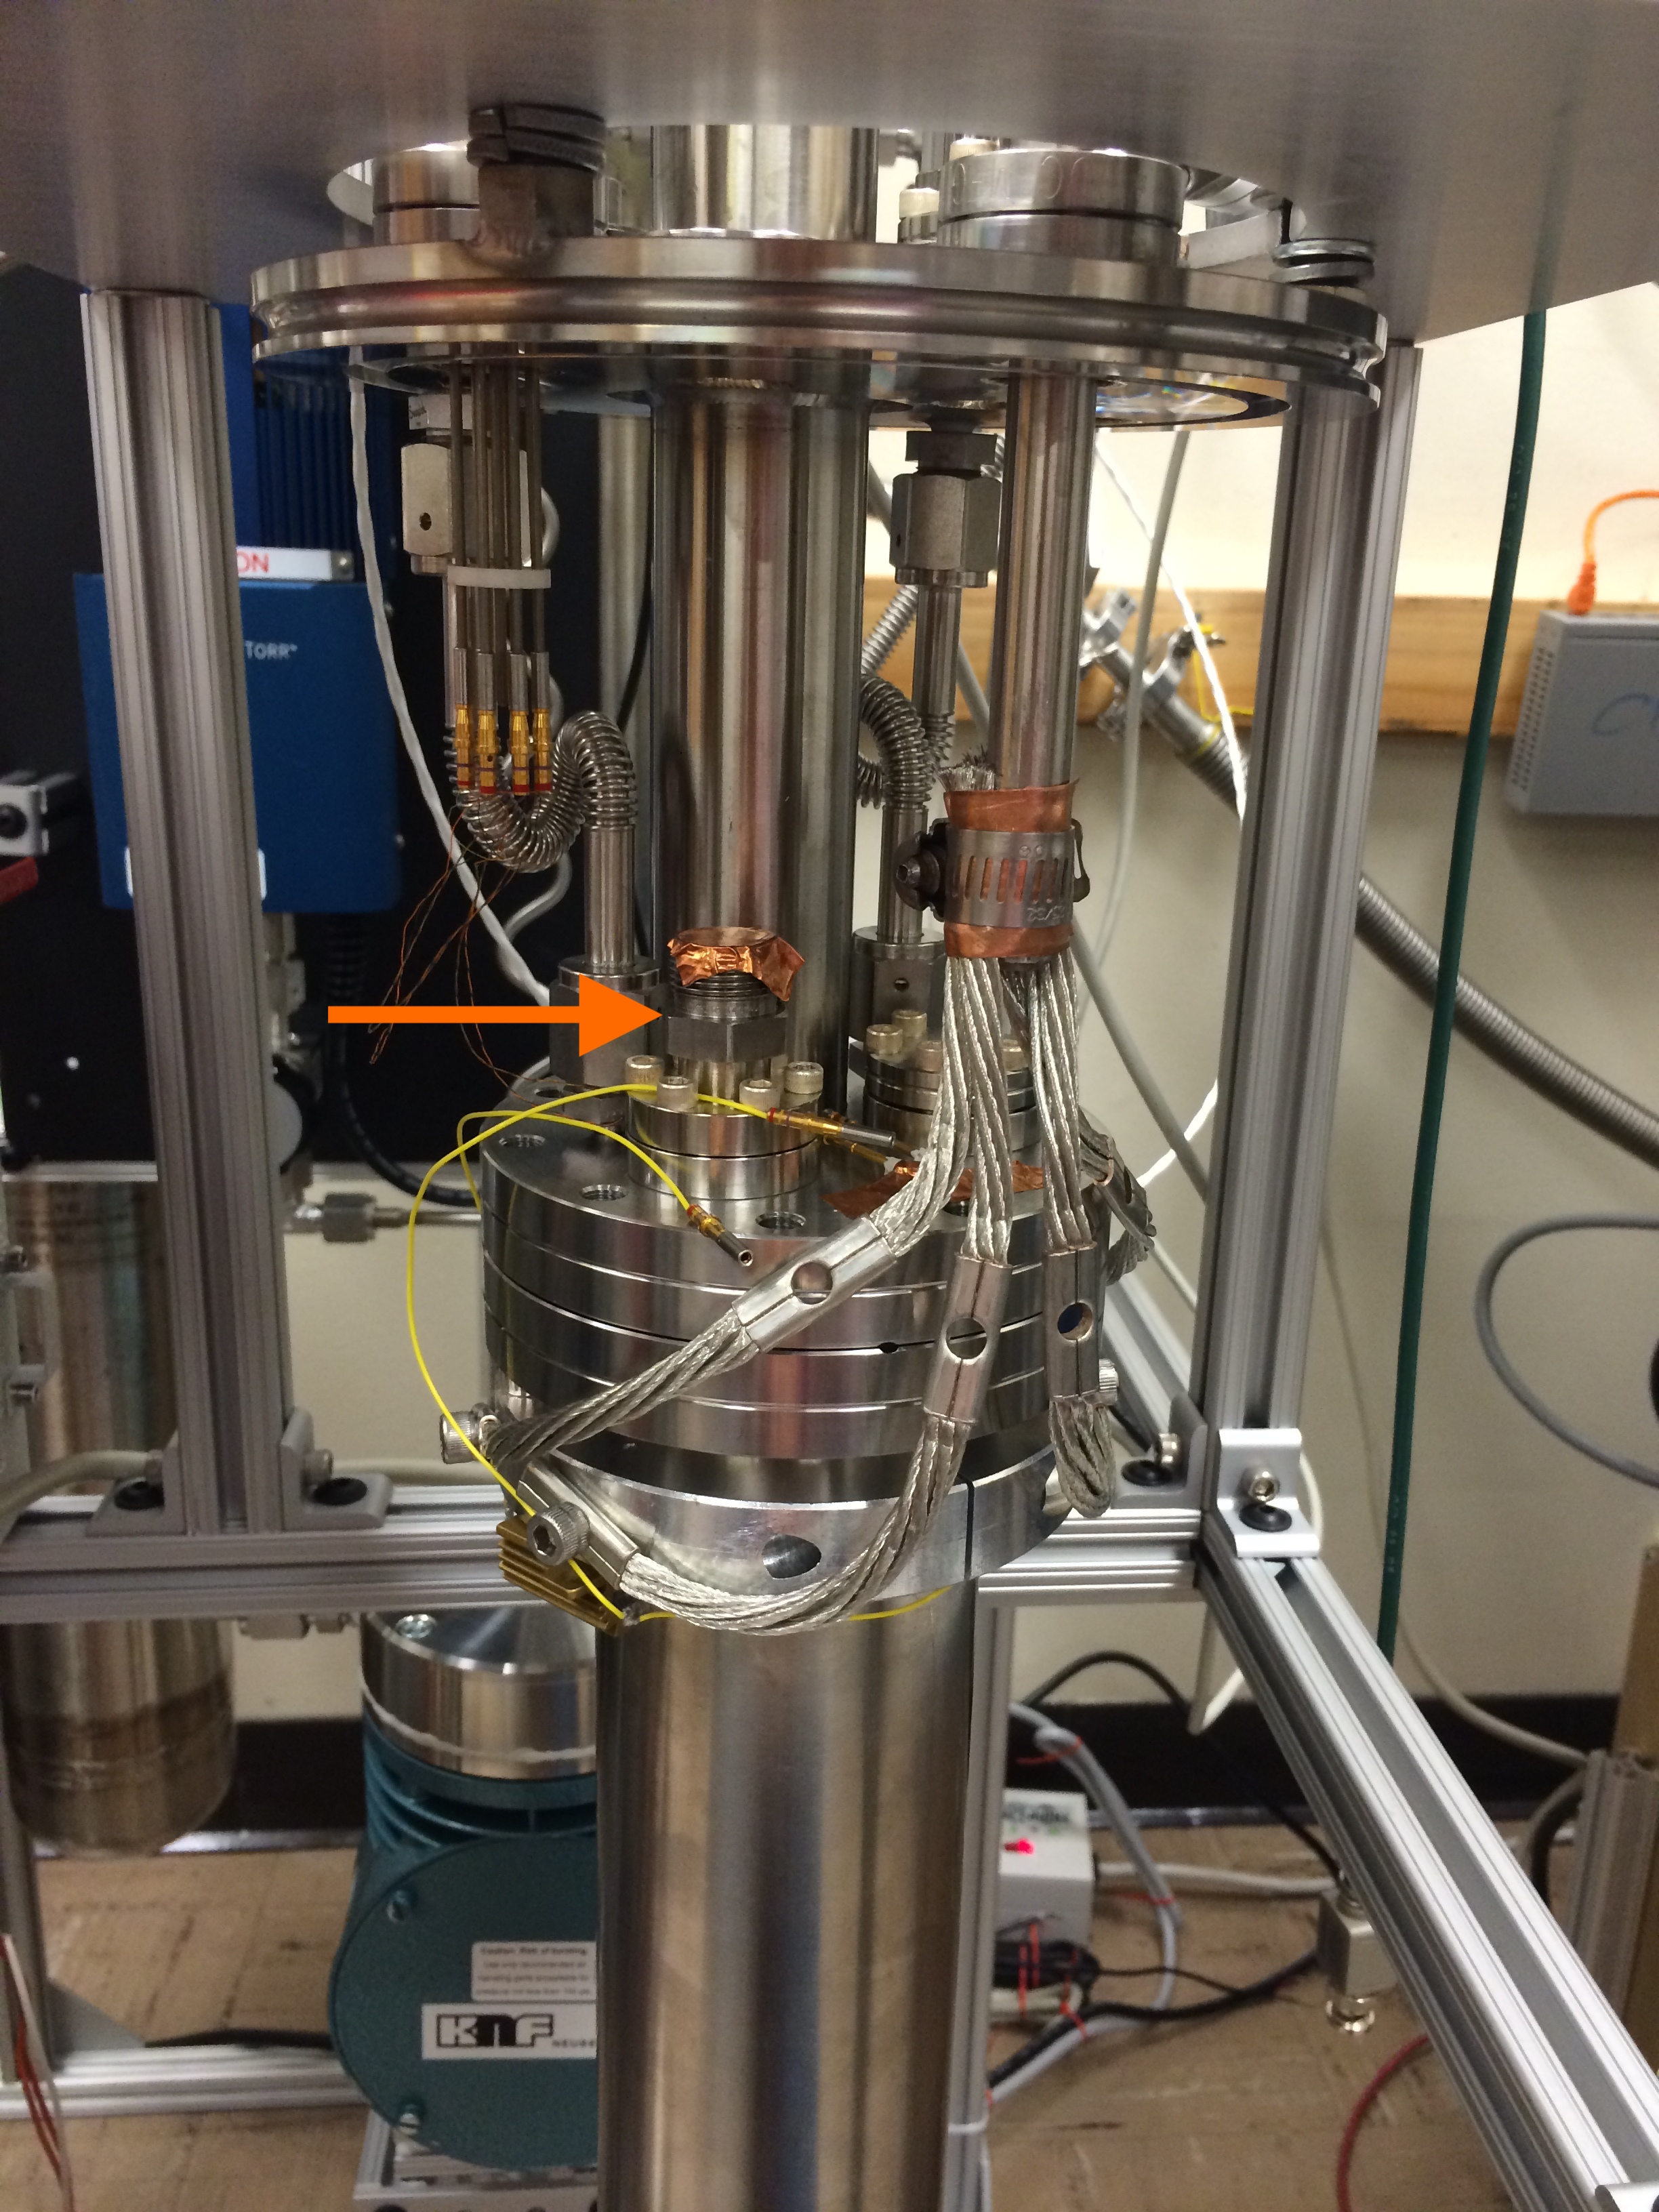
\includegraphics[width=3in]{figures/testbed/ft1_2.jpg}
\caption{The copper tape in this picture is sitting on top of a 1/2~-in swage connector. The swage connector captures a 1/2~in pipe, which has the 12kV SHV feedthrough welded to the end.}
\label{fig:ft1_2}
\end{center}
\end{figure}

\begin{figure}[htbp]
\begin{center}
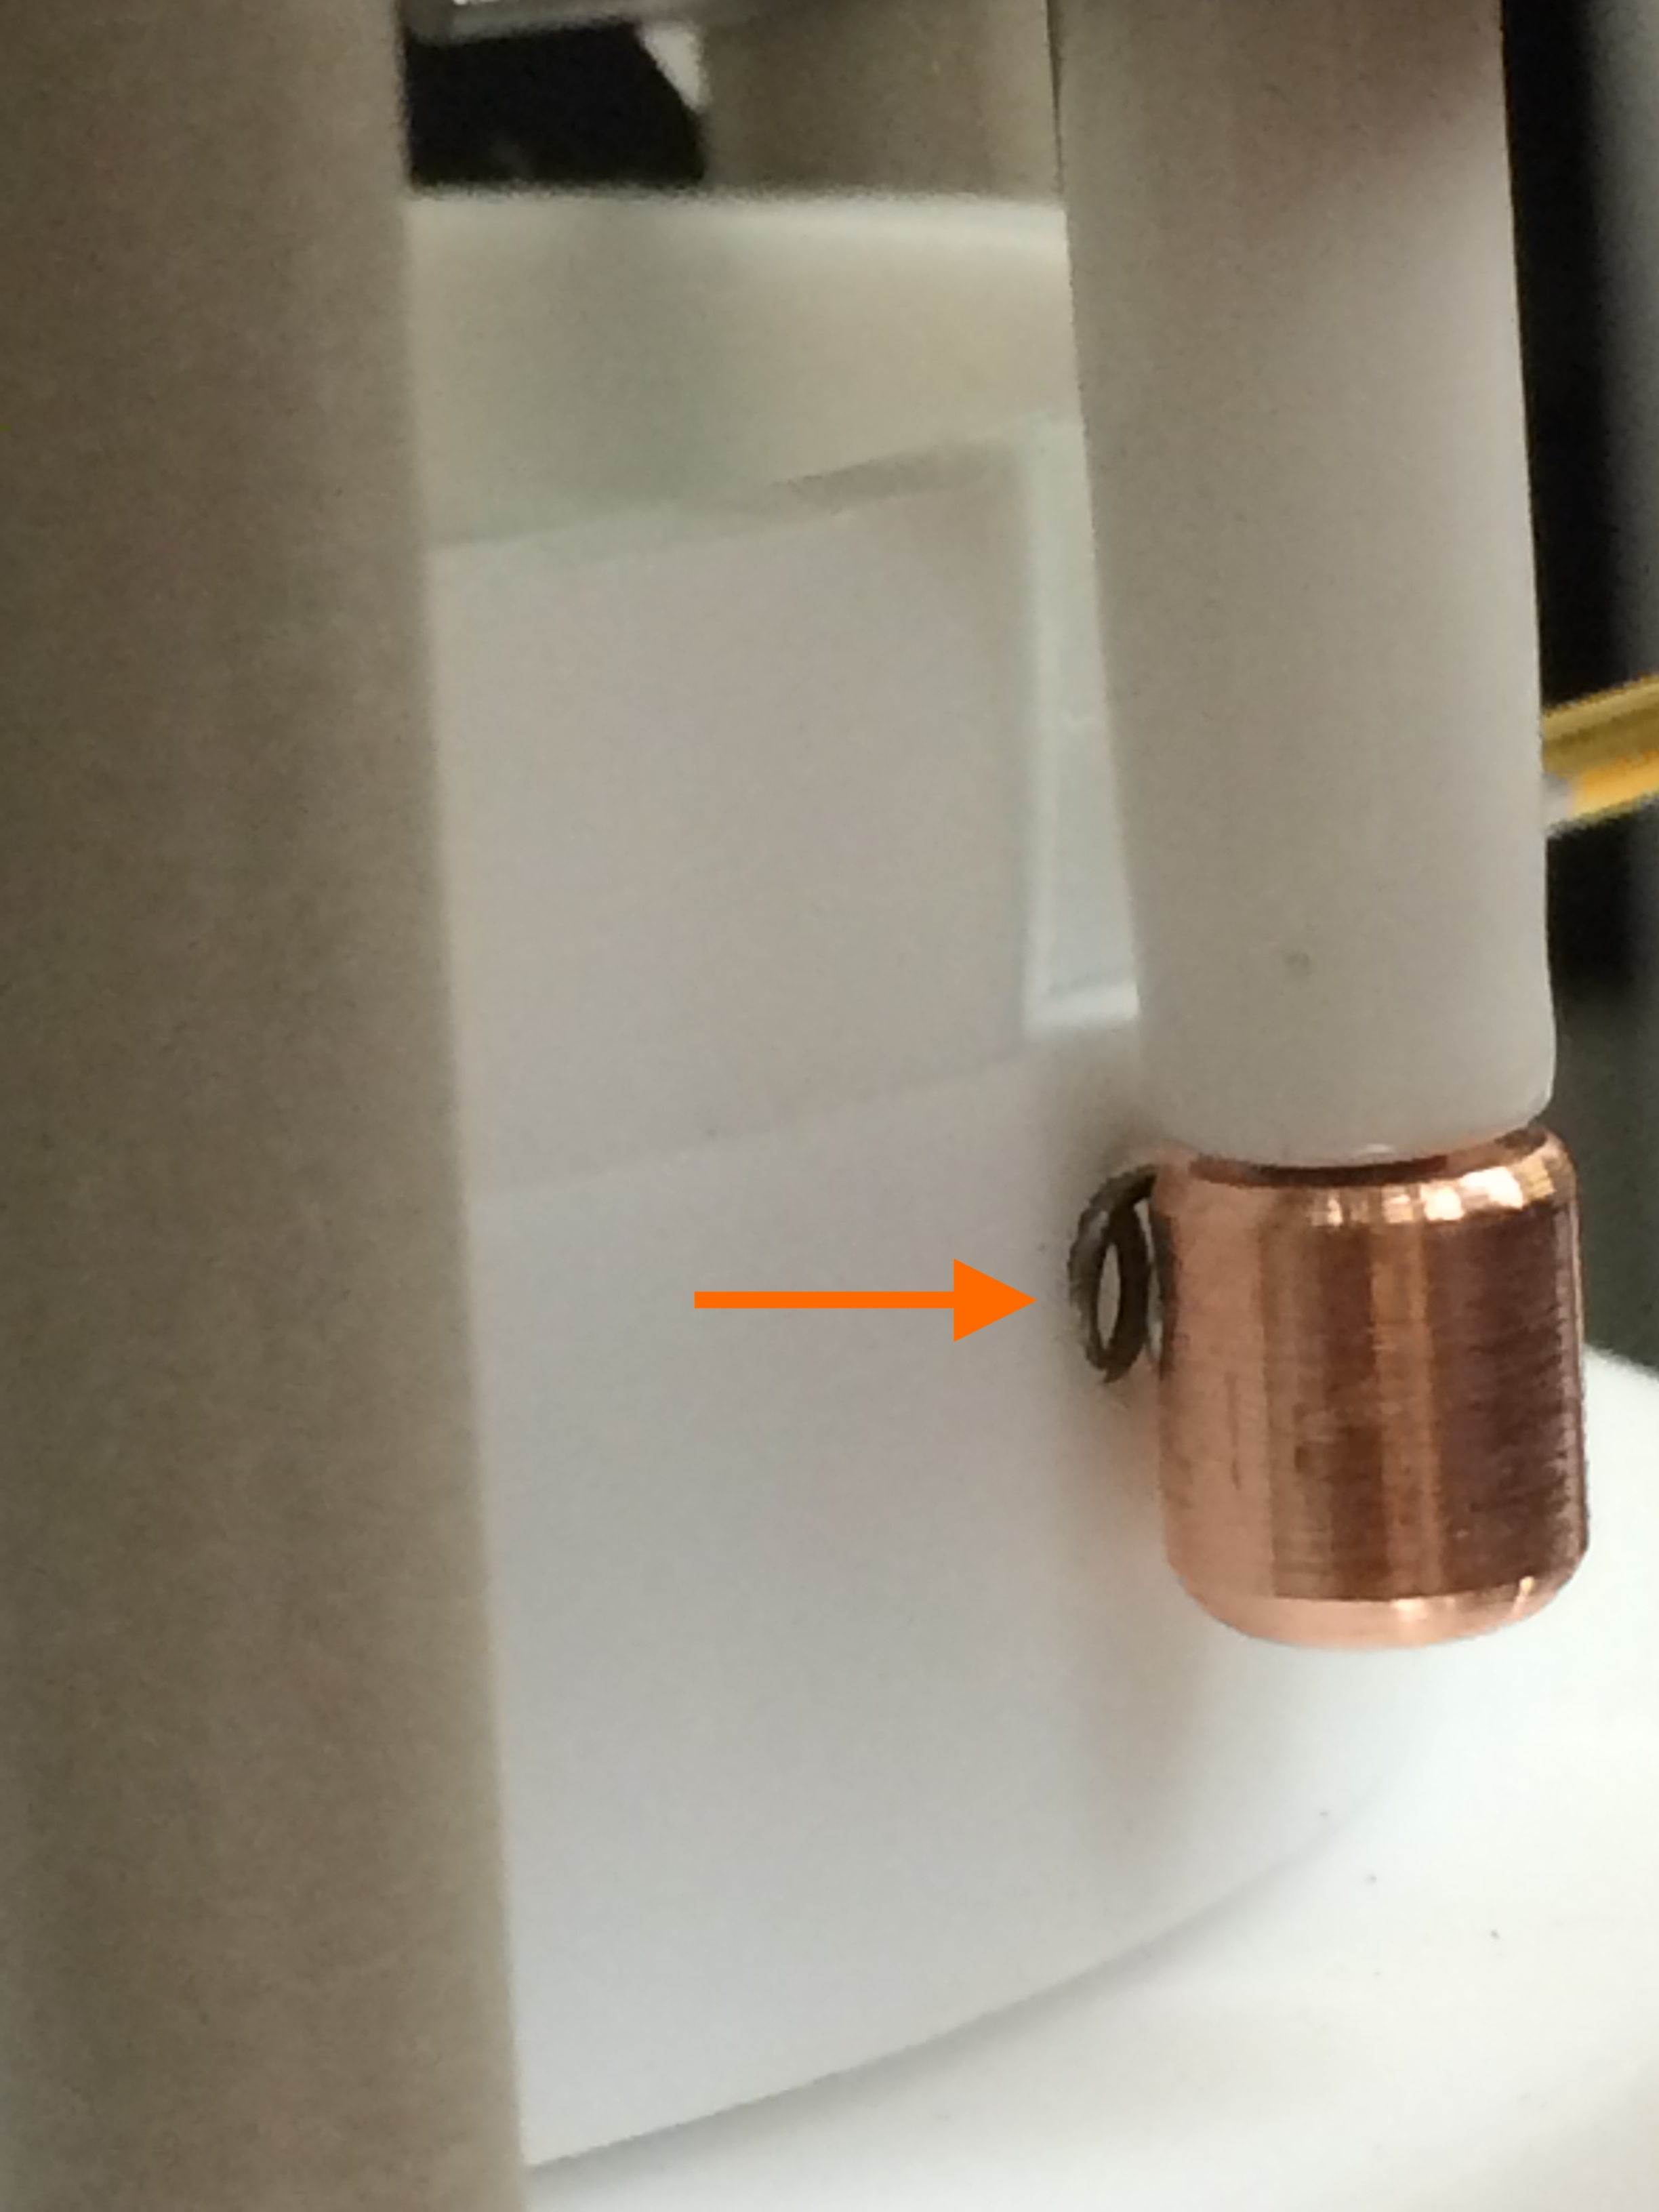
\includegraphics[width=\halffig]{figures/testbed/ft2_1.jpg}
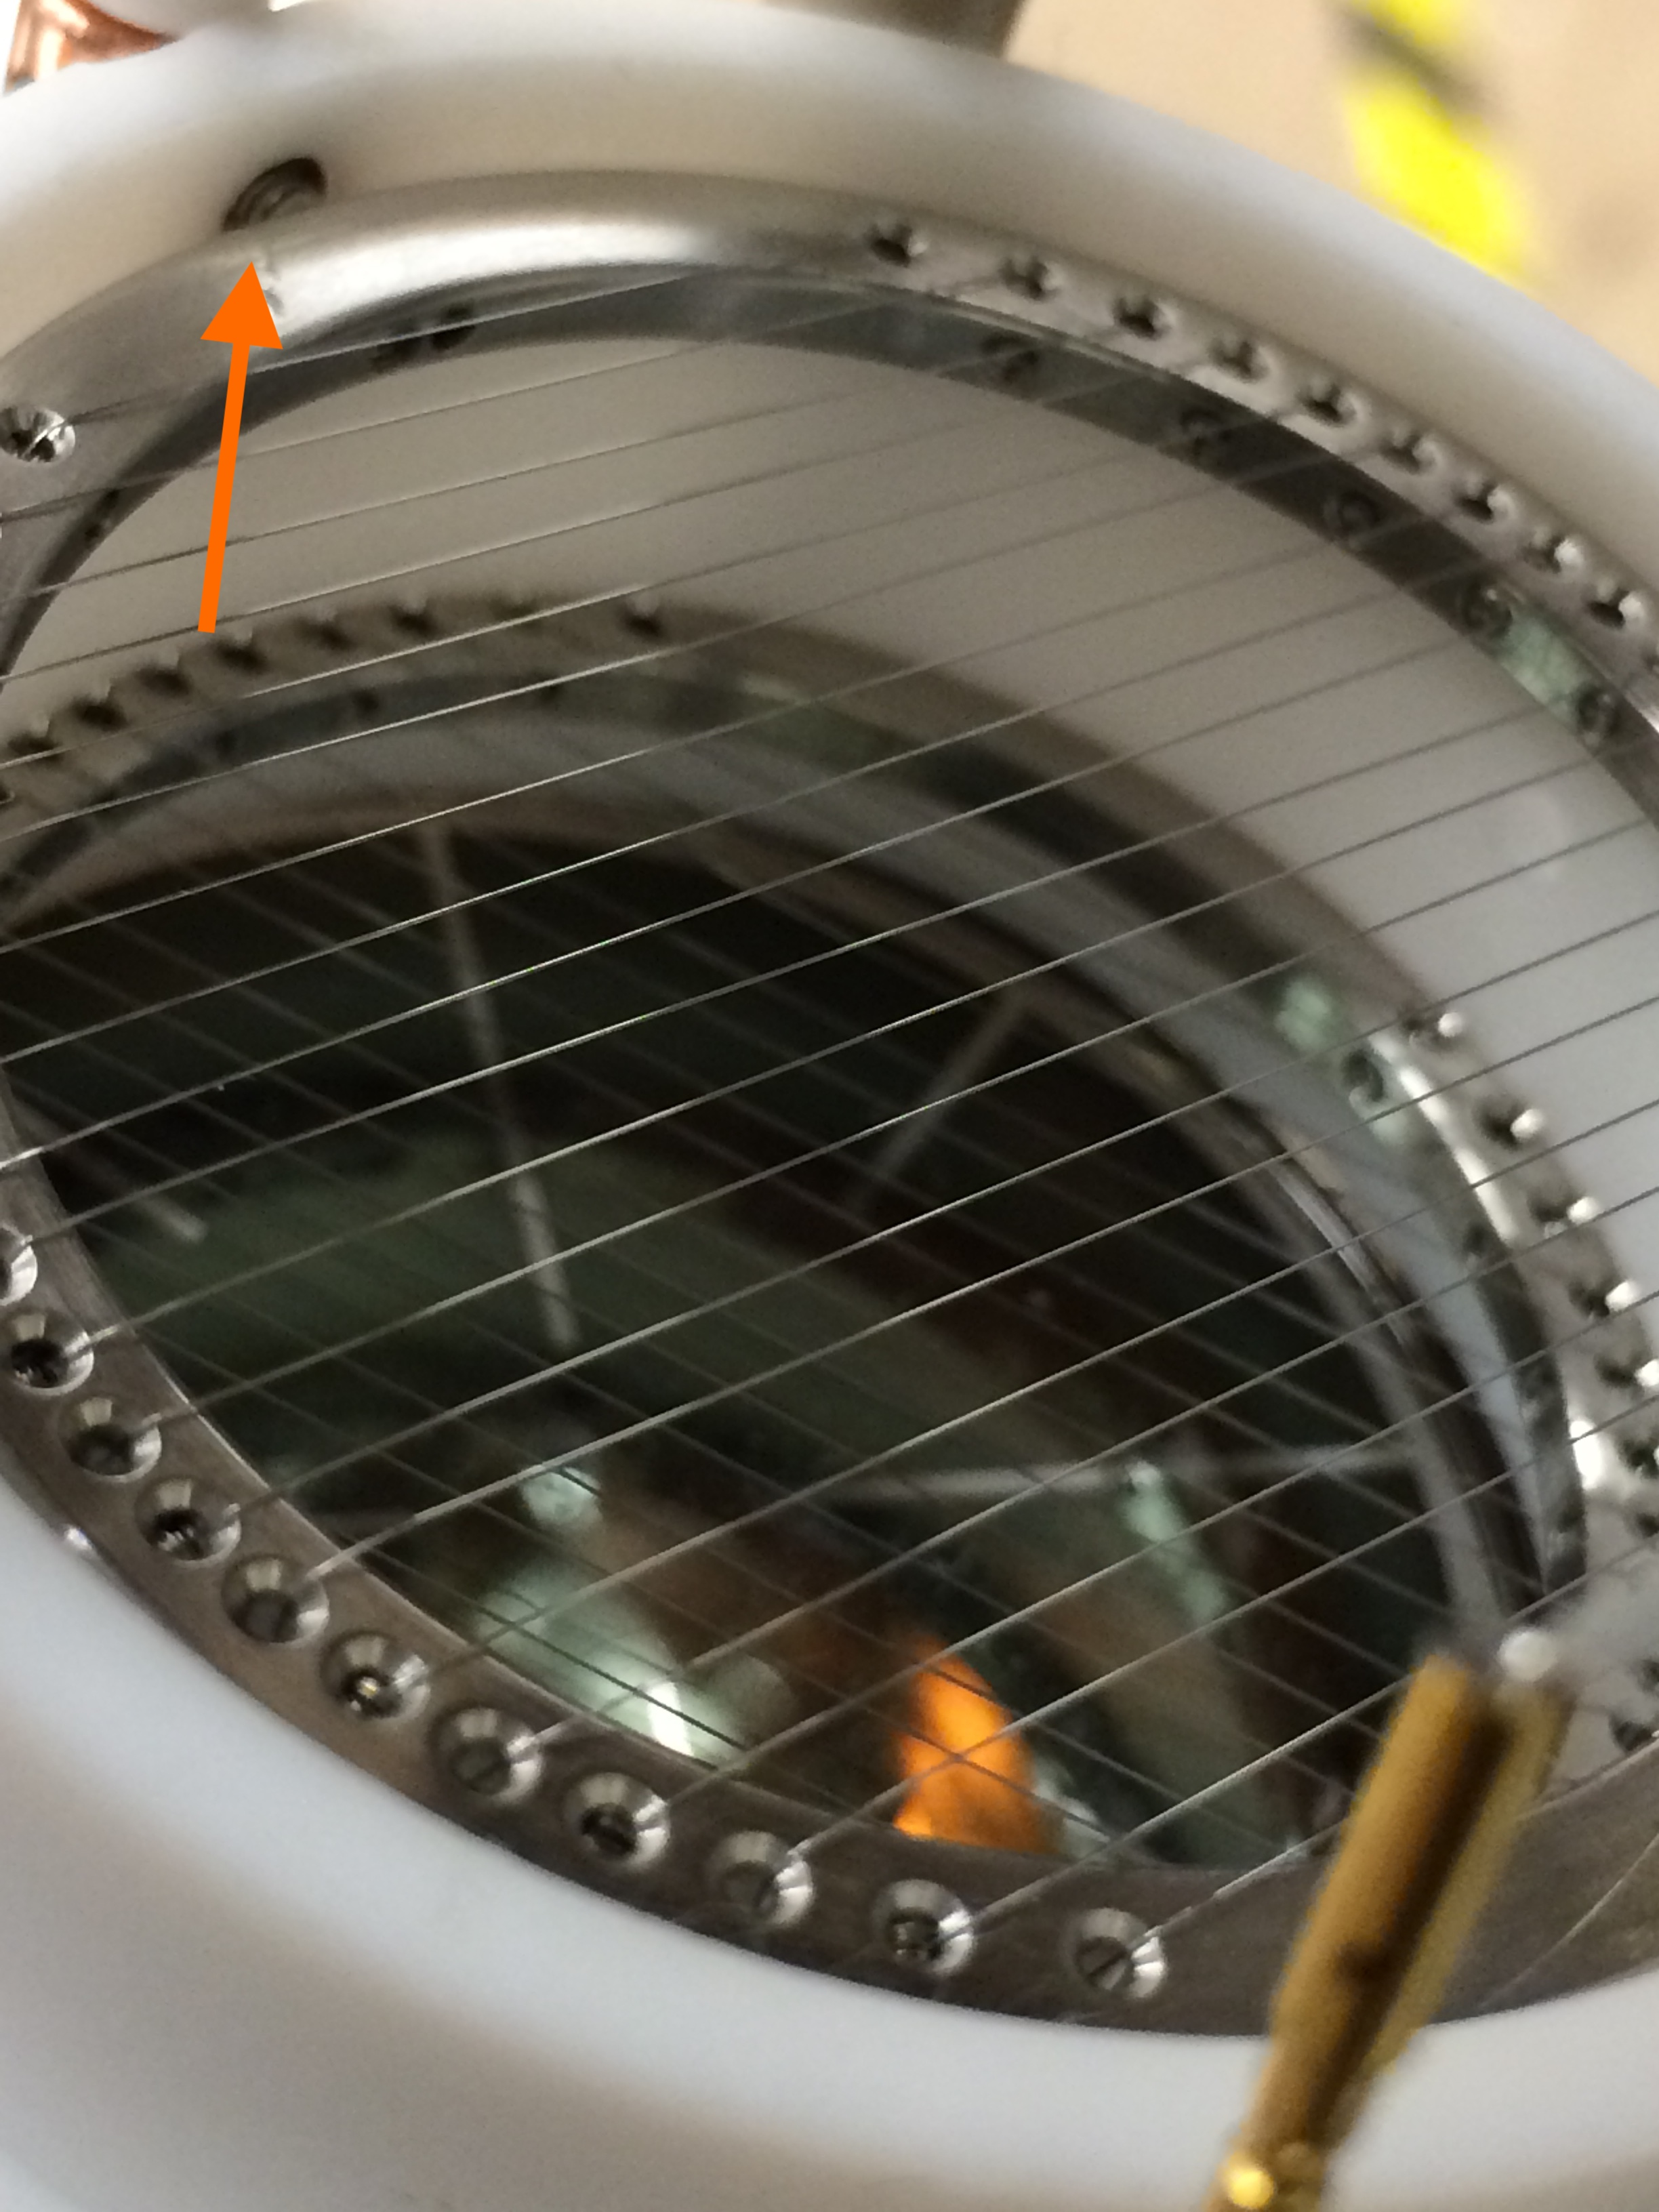
\includegraphics[width=\halffig]{figures/testbed/ft2_2.jpg}
\caption{The same 12kV SHV feed through, now with a modified spring connection connecting the feed through to the grid frame. A close up of the cathode grid showing the spring connection is on the \textbf{right}}
\label{fig:ft2_1}
\end{center}
\end{figure}


Feed throughs were tested by performing a cool down, ramping the \ac{HV} supply slowly, and watching an oscilloscope for a higher than baseline photon rate Figure~\ref{fig:phog} or a full xenon breakdown Figure~\ref{fig:breakdown}. The effect of raising the voltage on the \ac{HV} supply at a specific rate was also tested, and it was determined that the extremely slow and steady rate of a computer program was not necessarily superior to the imperfect method of the human experimenter -- the construction of the feed through, itself, outweighed any gains from computer-supervised voltage ramping.  


\begin{figure}[htbp]
\begin{center}
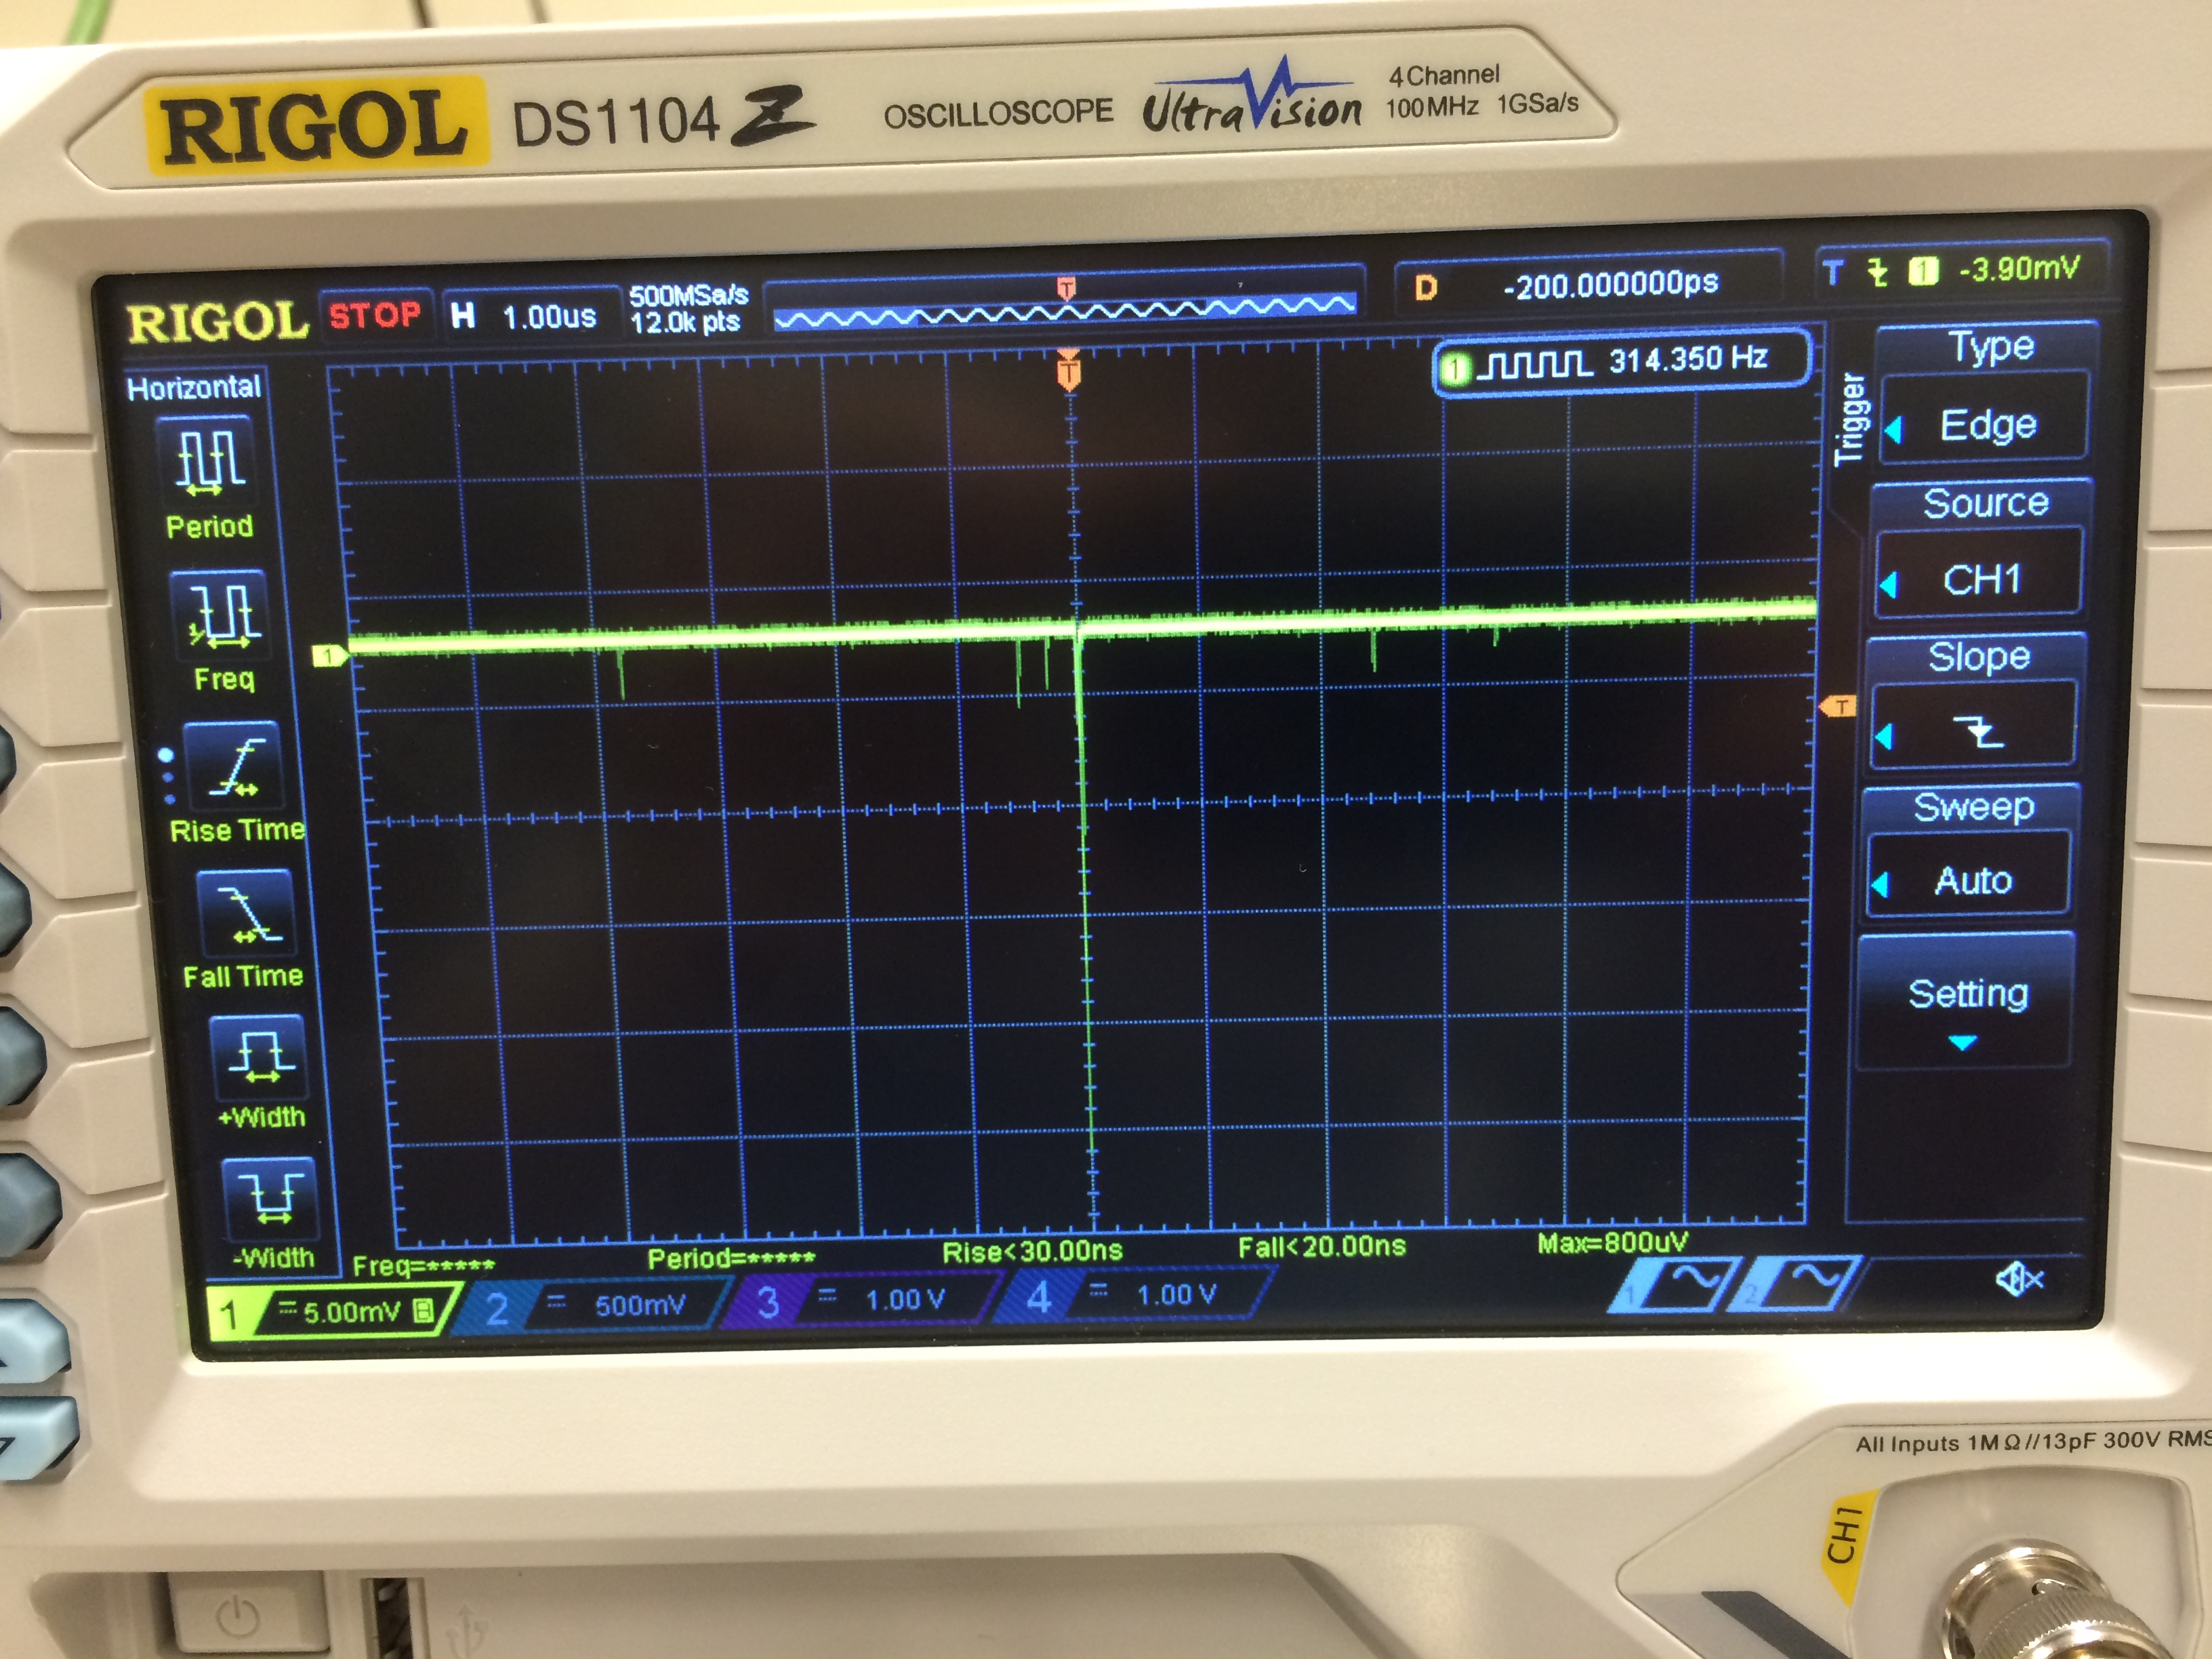
\includegraphics[width=\halffig]{figures/testbed/baseline.jpg}
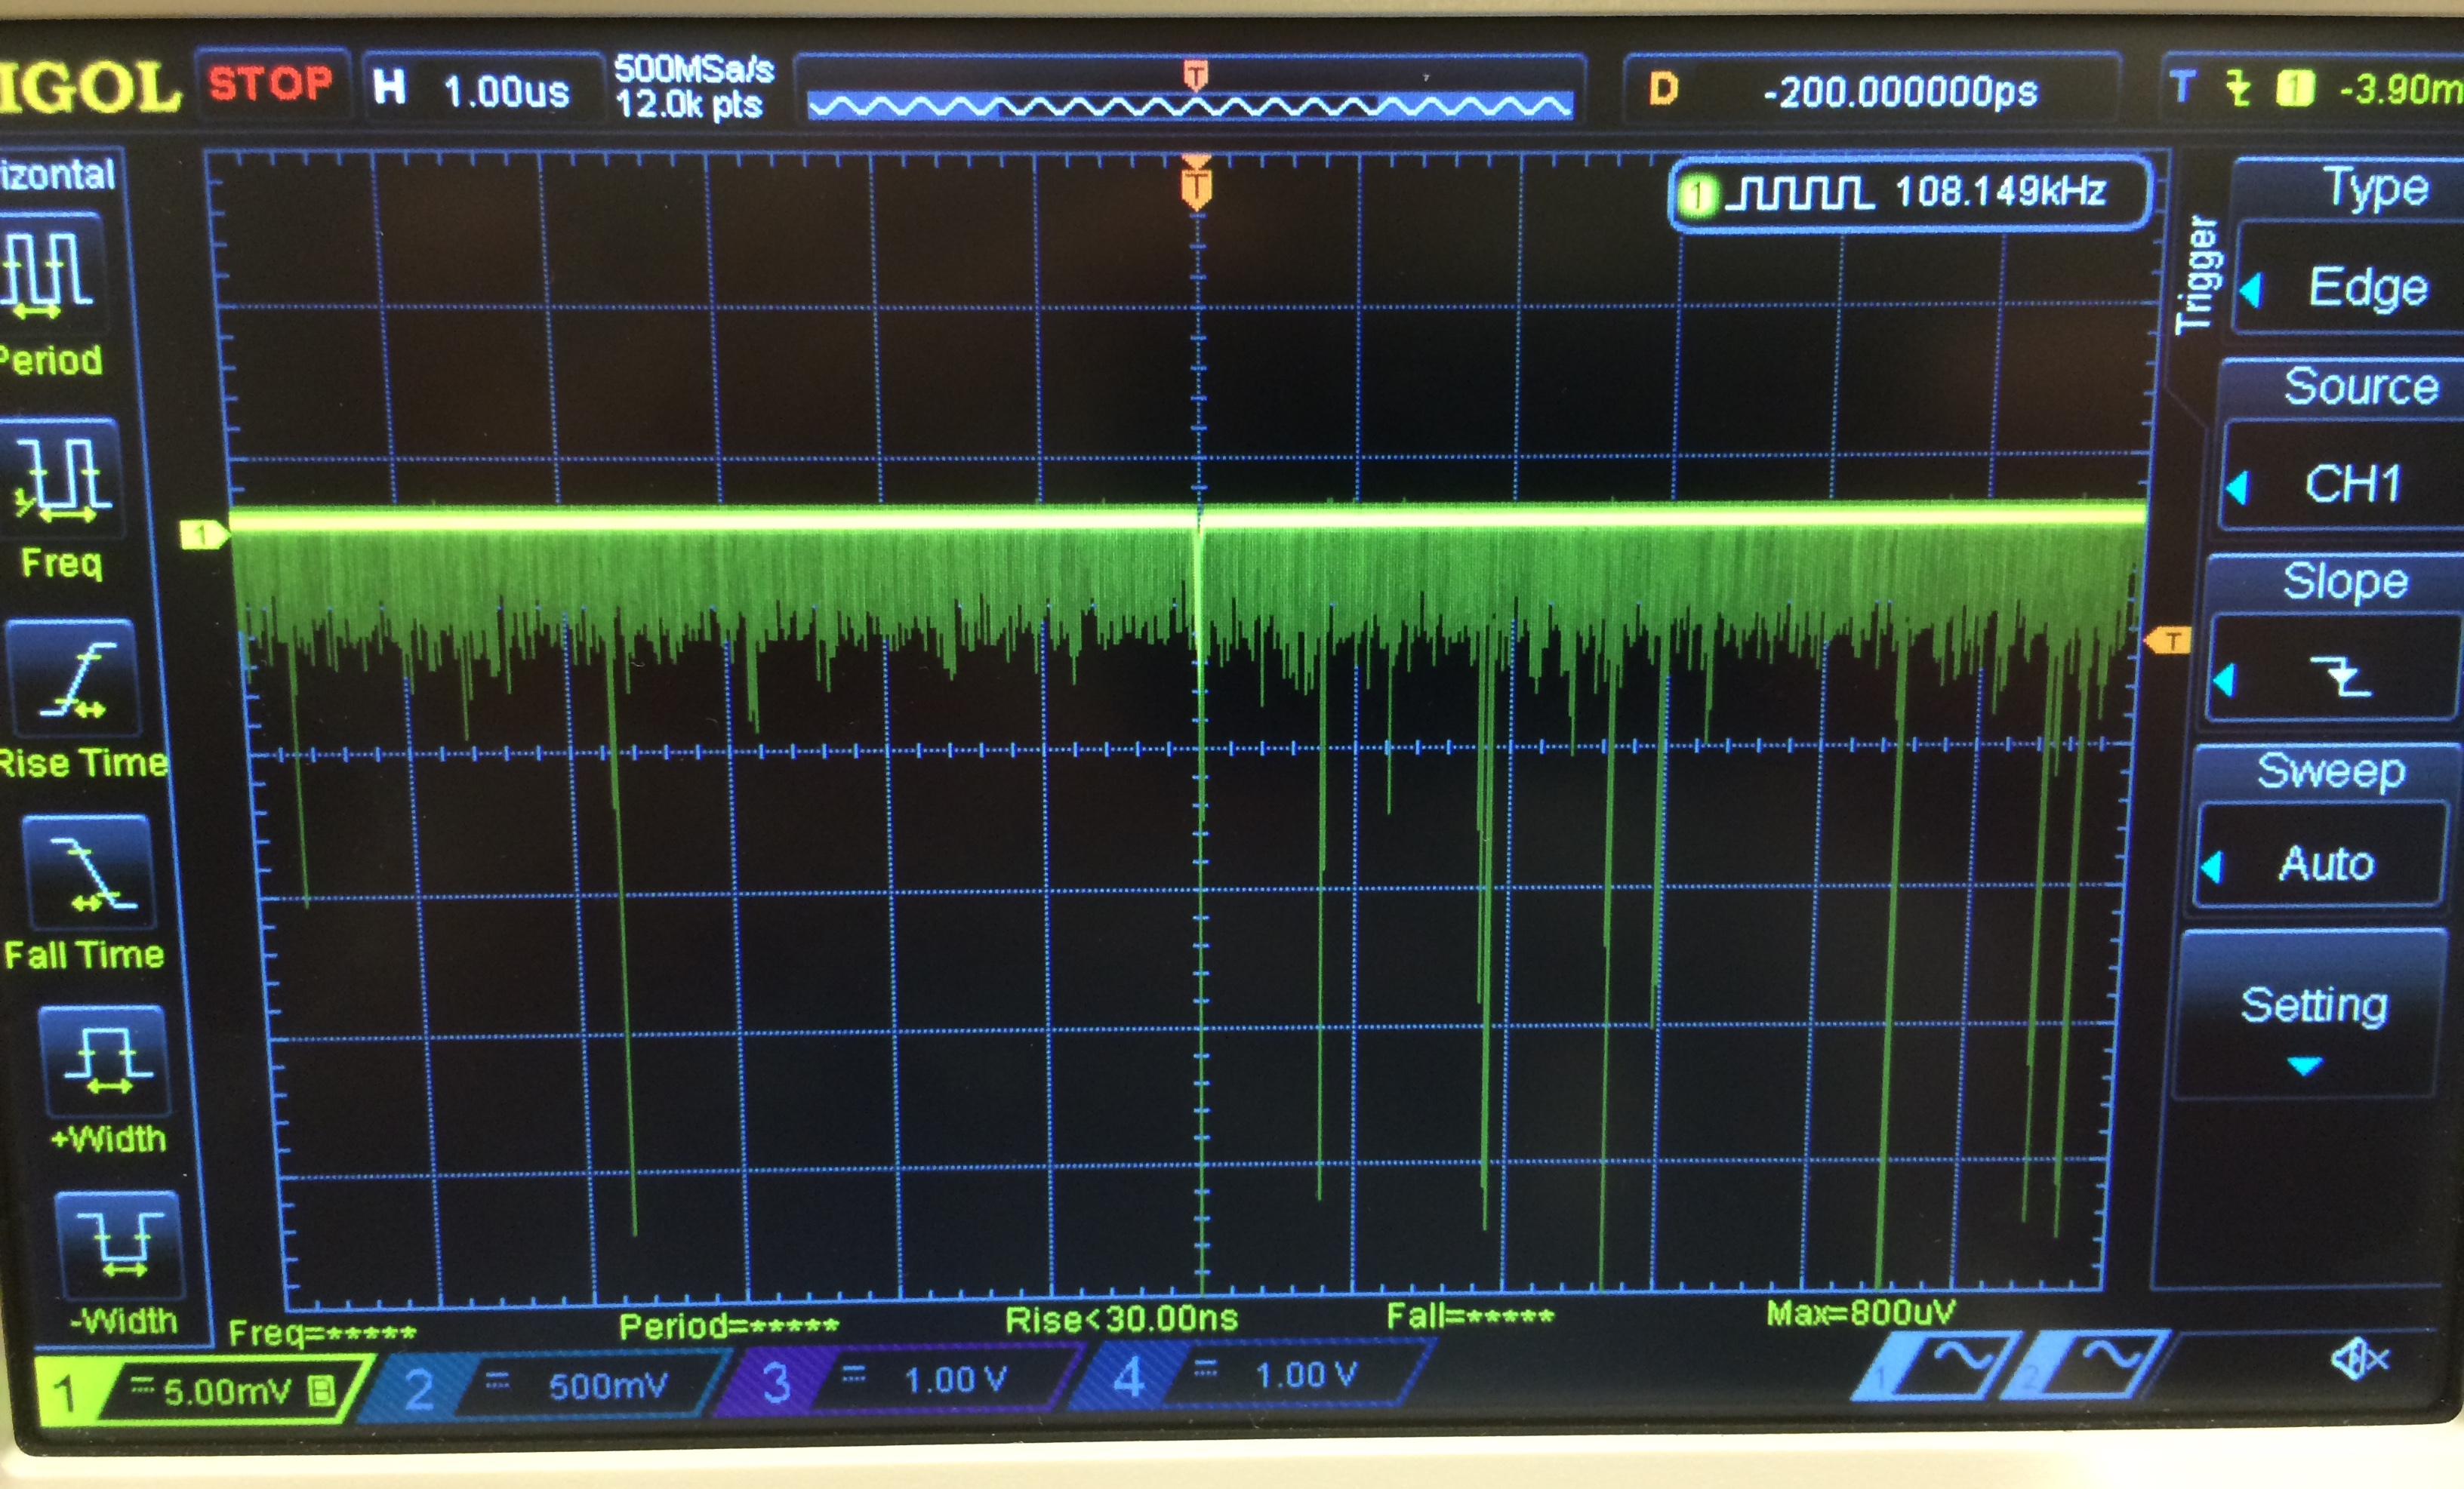
\includegraphics[width=\halffig]{figures/testbed/phog.jpg}
\caption{Oscilloscope showing baseline rate of single photons (left) compared to a high rate of single photons (right) caused by the high voltage feed through.}
\label{fig:phog}
\end{center}
\end{figure}


\begin{figure}[htbp]
\begin{center}
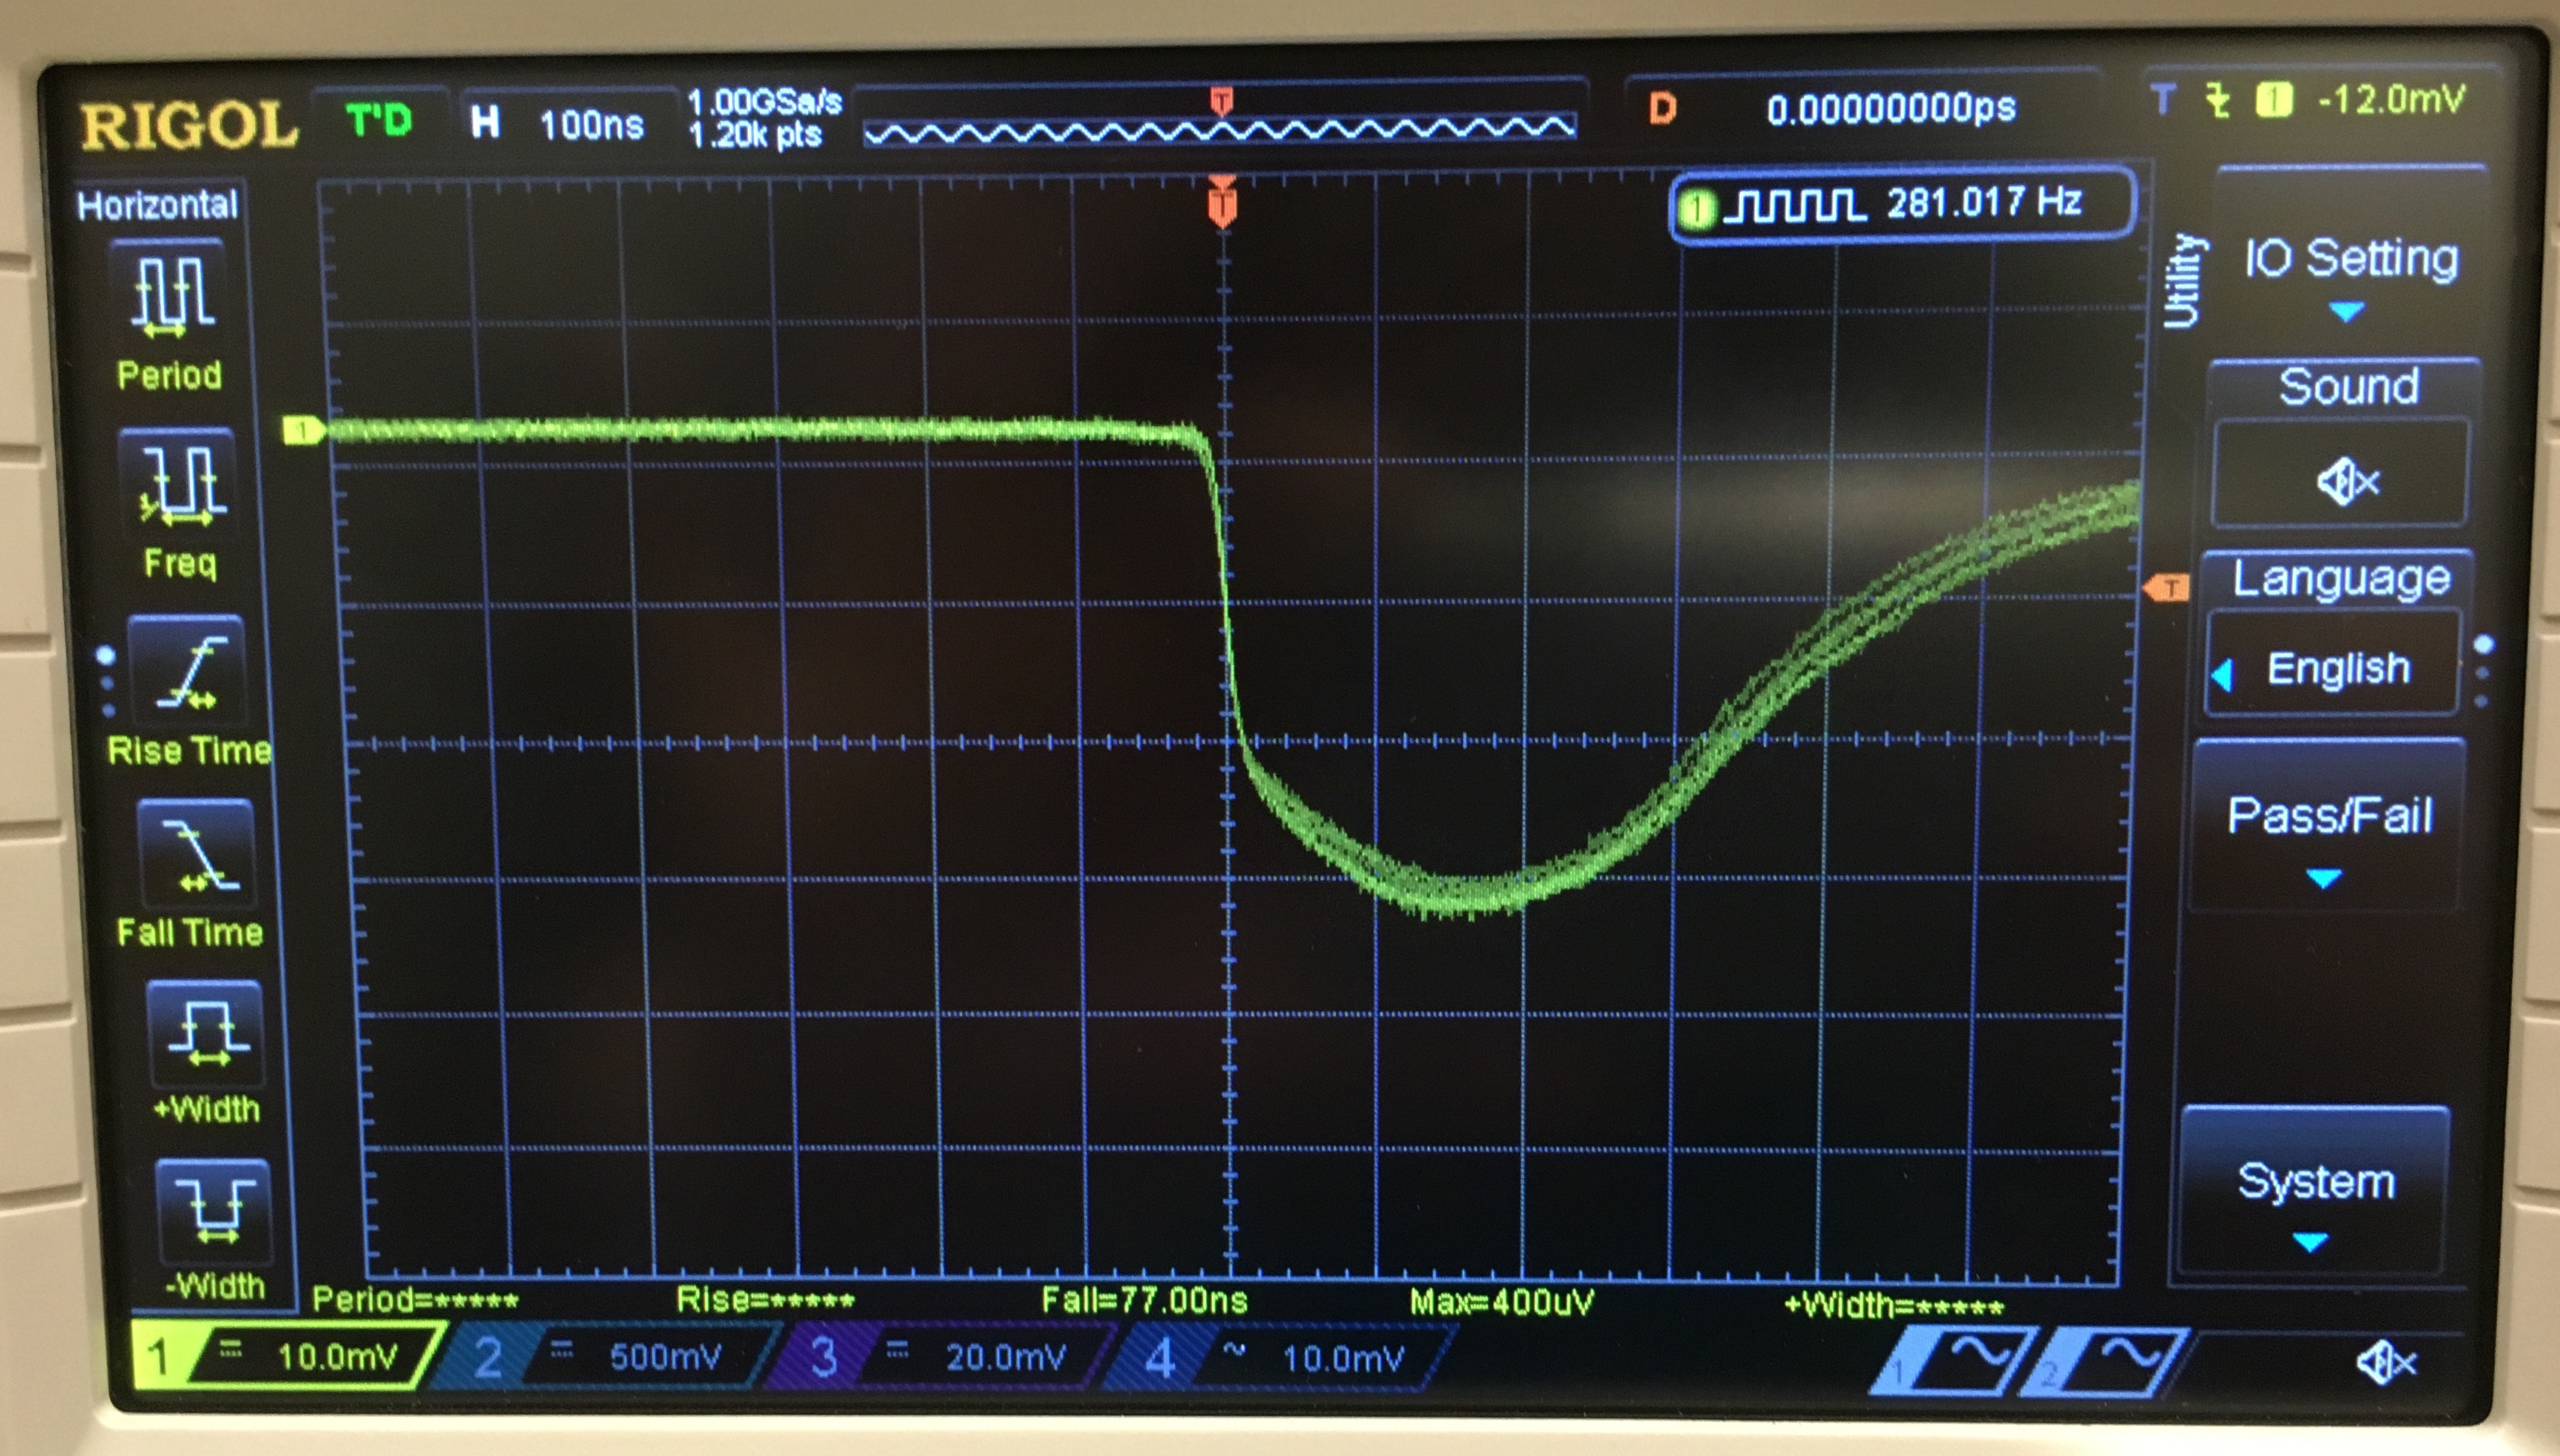
\includegraphics[width=\halffig]{figures/testbed/breakdown.jpg}
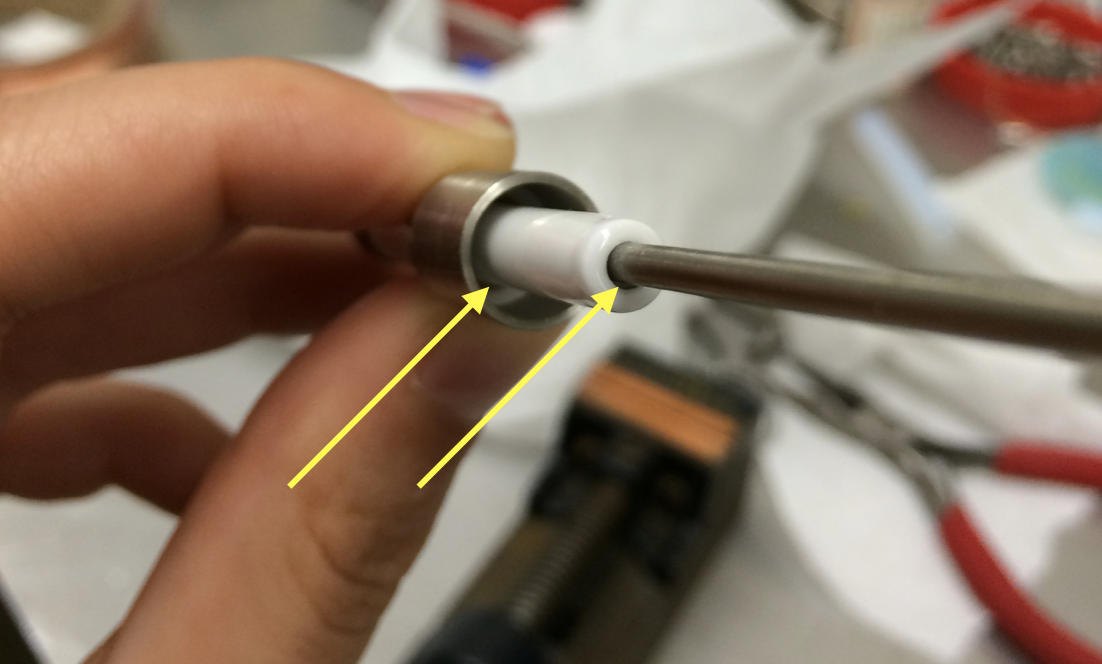
\includegraphics[width=\halffig]{figures/testbed/ft_1and2_gasgaps.png}

\caption{(Left) Full xenon breakdown as visible on the PMT trace. The large, saturated pulse is caused by the high intensity of light. This type of breakdown was often accompanied by an audible buzz, and a rise in current that would initiate a trip of the high voltage supply. (Right) a close up of the xenon-facing side of the feedthrough. Visible gaps where xenon gas is exposed to high fields are particularly problematic for breakdowns.}
\label{fig:breakdown}
\end{center}
\end{figure}

Iterations of the 12kV SHV feed though were not able to reach more than about 9kV, and not more than about 7kV for extended periods of time like those that would be required for data acquisition. A summary of the issues with this type of feed through design is given below:
\begin{itemize}
\item Gas gaps
\item Triple points
\item Prone to aging
\end{itemize}

We also tried a stock 20kV SHV feed through with a custom end cap designed by a \ac{HV} engineer, meant to smooth out typical triple point issues. This feed through was mounted on a CF flange far from the active region. A length of cable was stripped of grounding sheath for its entire length. A small section on one end was stripped of dielectric, this end was tied to the SHV feed though with copper wire, and the custom end cap was placed over this. The side of the cable making the connection to the cathode grid was drilled out for a short length on the bottom, leaving only a tube of dielectric with no conductor. A threaded rod was inserted into the cable, such that the rod made contact with the conductor. The cathode grid frame was screwed onto the threaded rod. The SHV-20 feed though is summarized in pictures in Figure~\ref{fig:shv20}, and was found to hold sufficient voltage (~10kV) for extended periods of time. However, it was found that the voltage capability of this feed though decreased over time; this is discussed in the next section.

\begin{figure}[htbp]
\begin{minipage}{0.47\textwidth}
    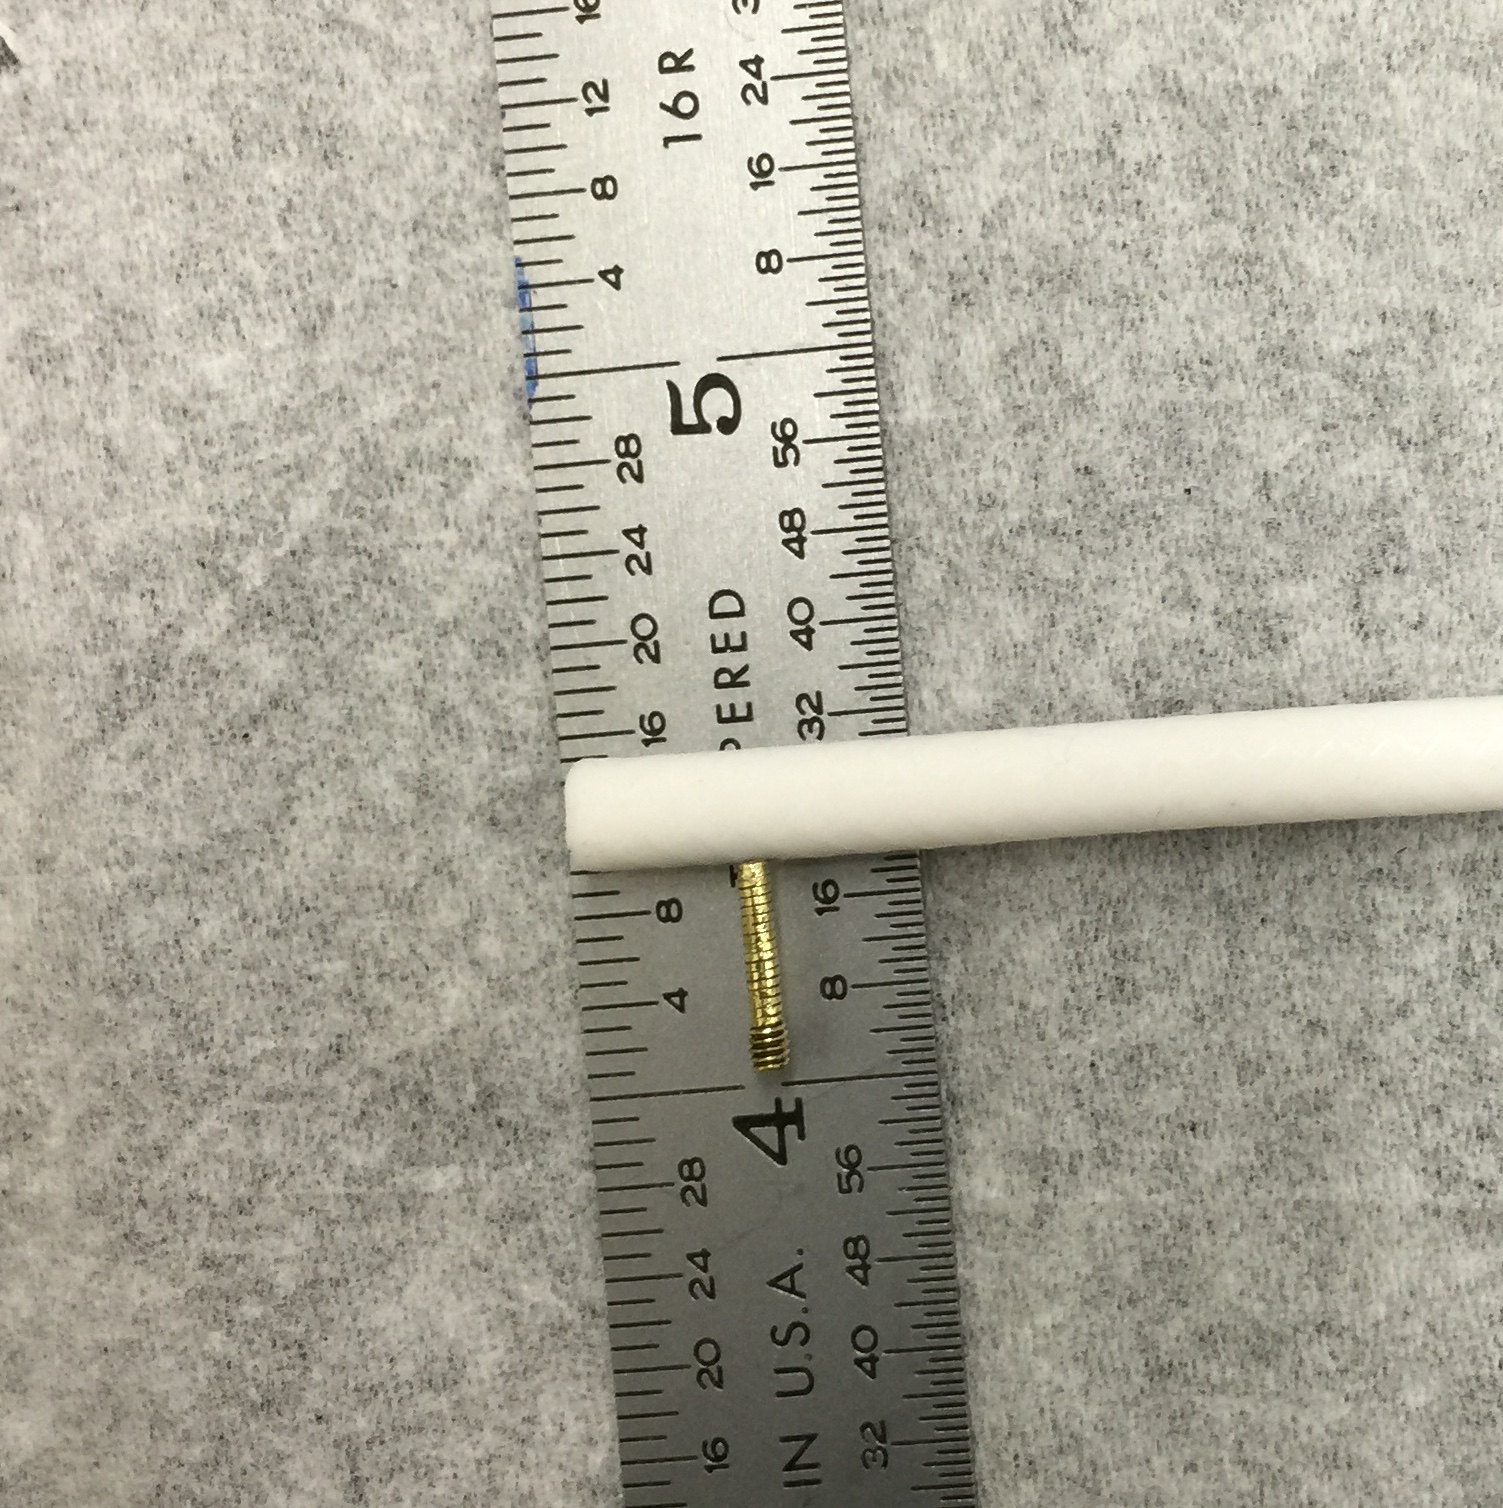
\includegraphics[width=\linewidth]{figures/testbed/ft3_1.jpg}
    \end{minipage}
    \hspace{\fill} % note: no blank line here
    \begin{minipage}{0.47\textwidth}
    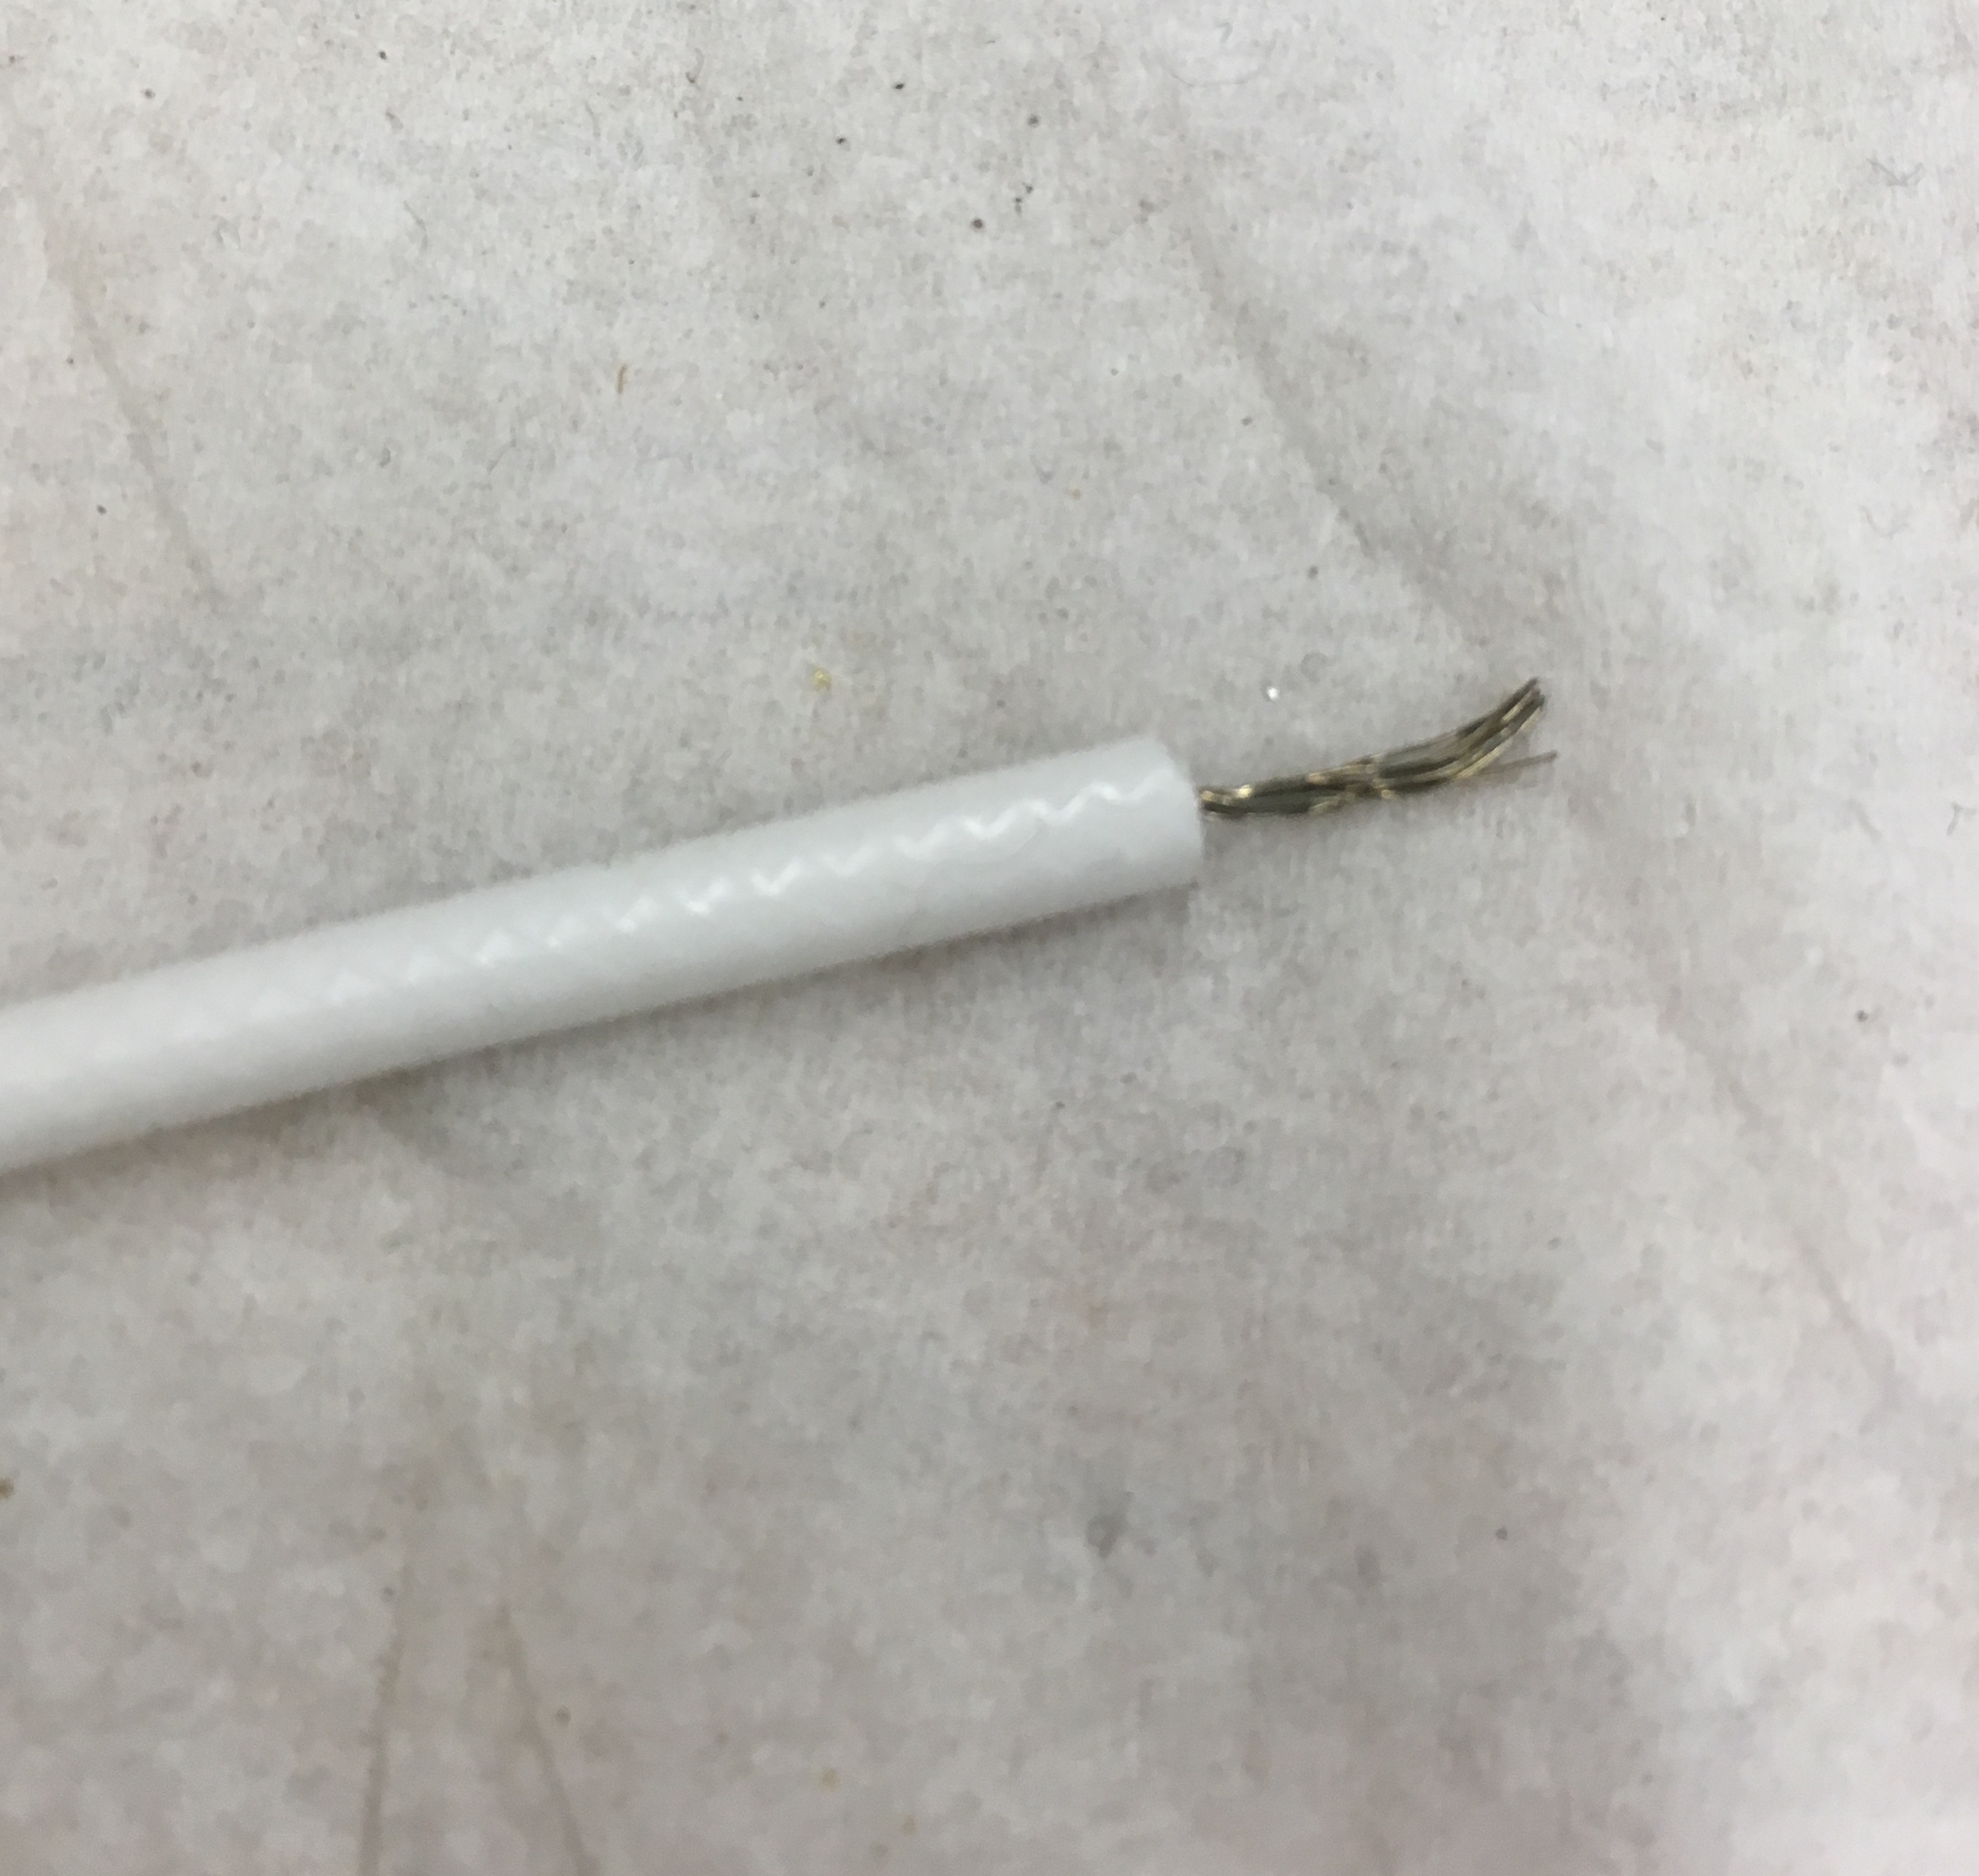
\includegraphics[width=\linewidth]{figures/testbed/ft3_2.jpg}
    \end{minipage}

    \vspace*{1cm} % vertical separation

    \begin{minipage}{0.47\textwidth}
    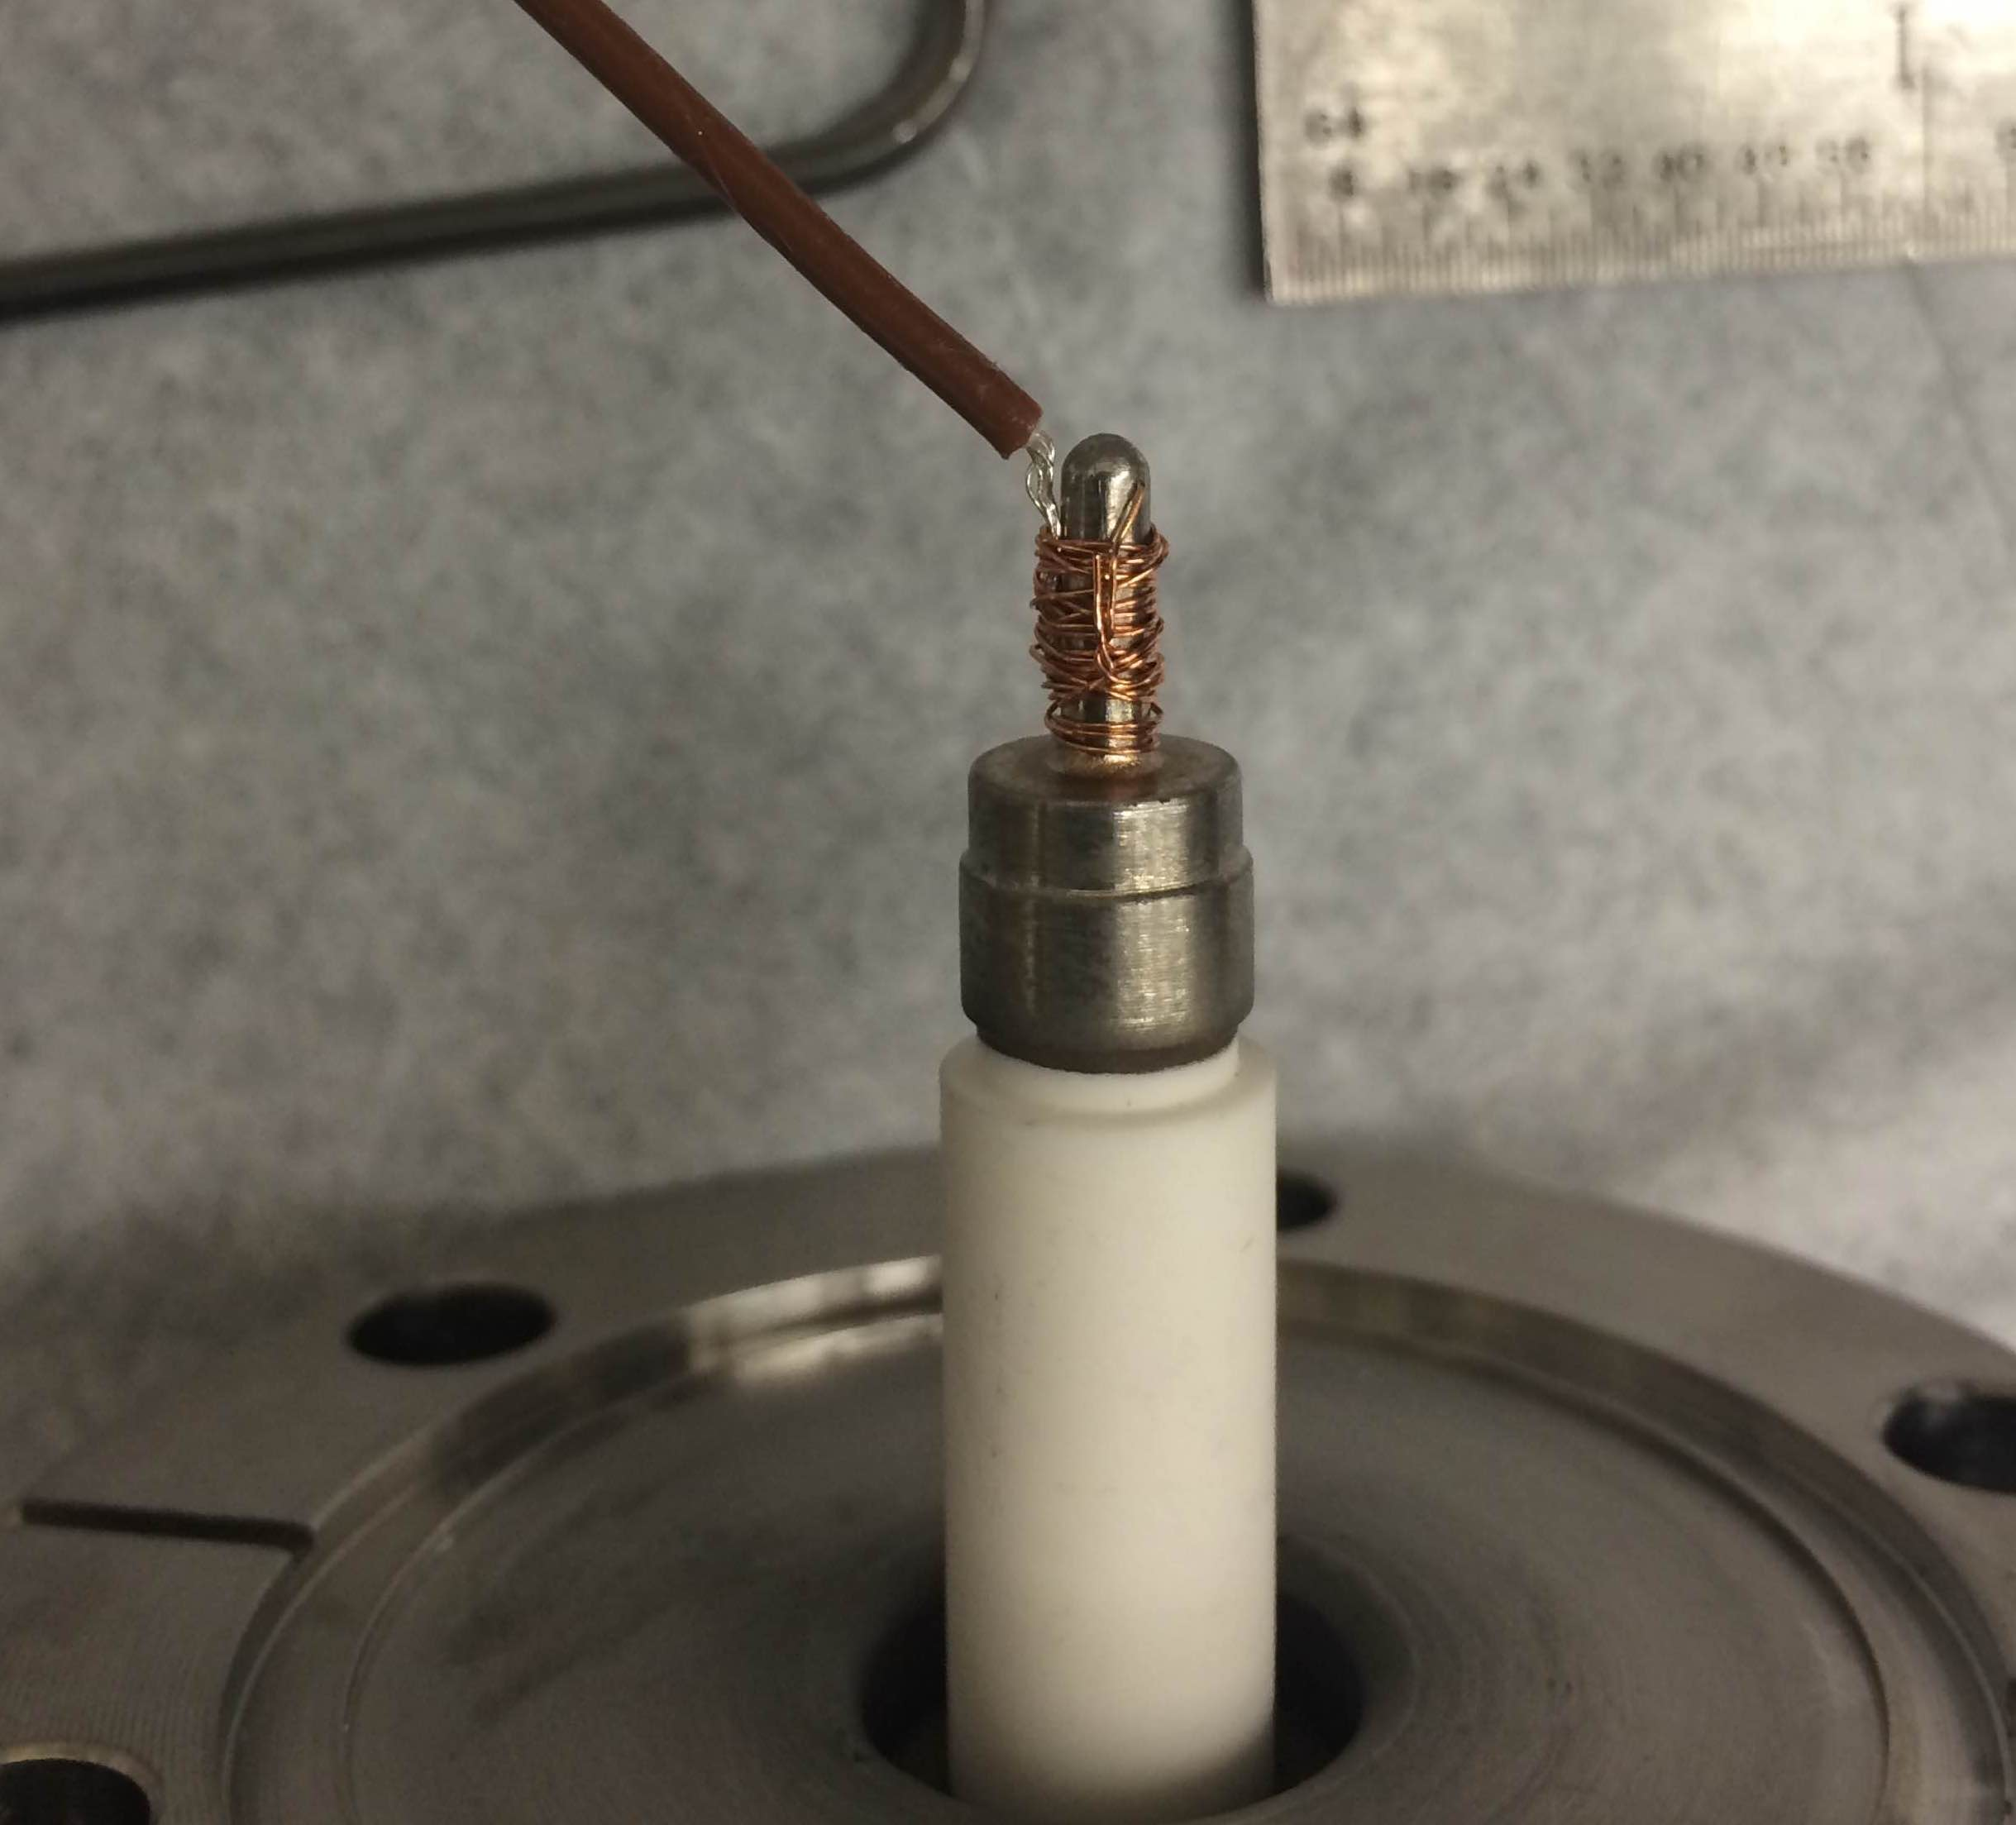
\includegraphics[width=\linewidth]{figures/testbed/ft3_3.jpg}
    \end{minipage}
    \hspace{\fill} % note: no blank line here
    \begin{minipage}{0.47\textwidth}
    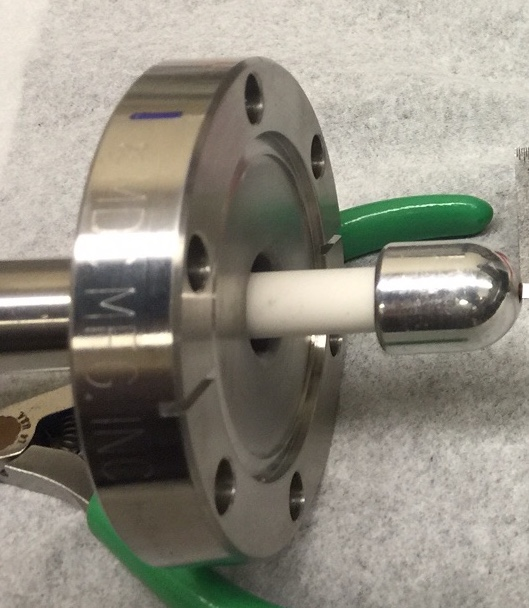
\includegraphics[width=\linewidth]{figures/testbed/ft3_4.jpg}
    \end{minipage}
\caption{Top: (left) cathode connection side (right) SHV-20 connection side Bottom: (left) an example showing how the cable was attached to the stock SHV-20 feed though end (right) a custom cap fit over the connection, smoothing out triple points.}
 \label{fig:shv20}
\end{figure}

 \begin{figure}[htbp]
\begin{center}
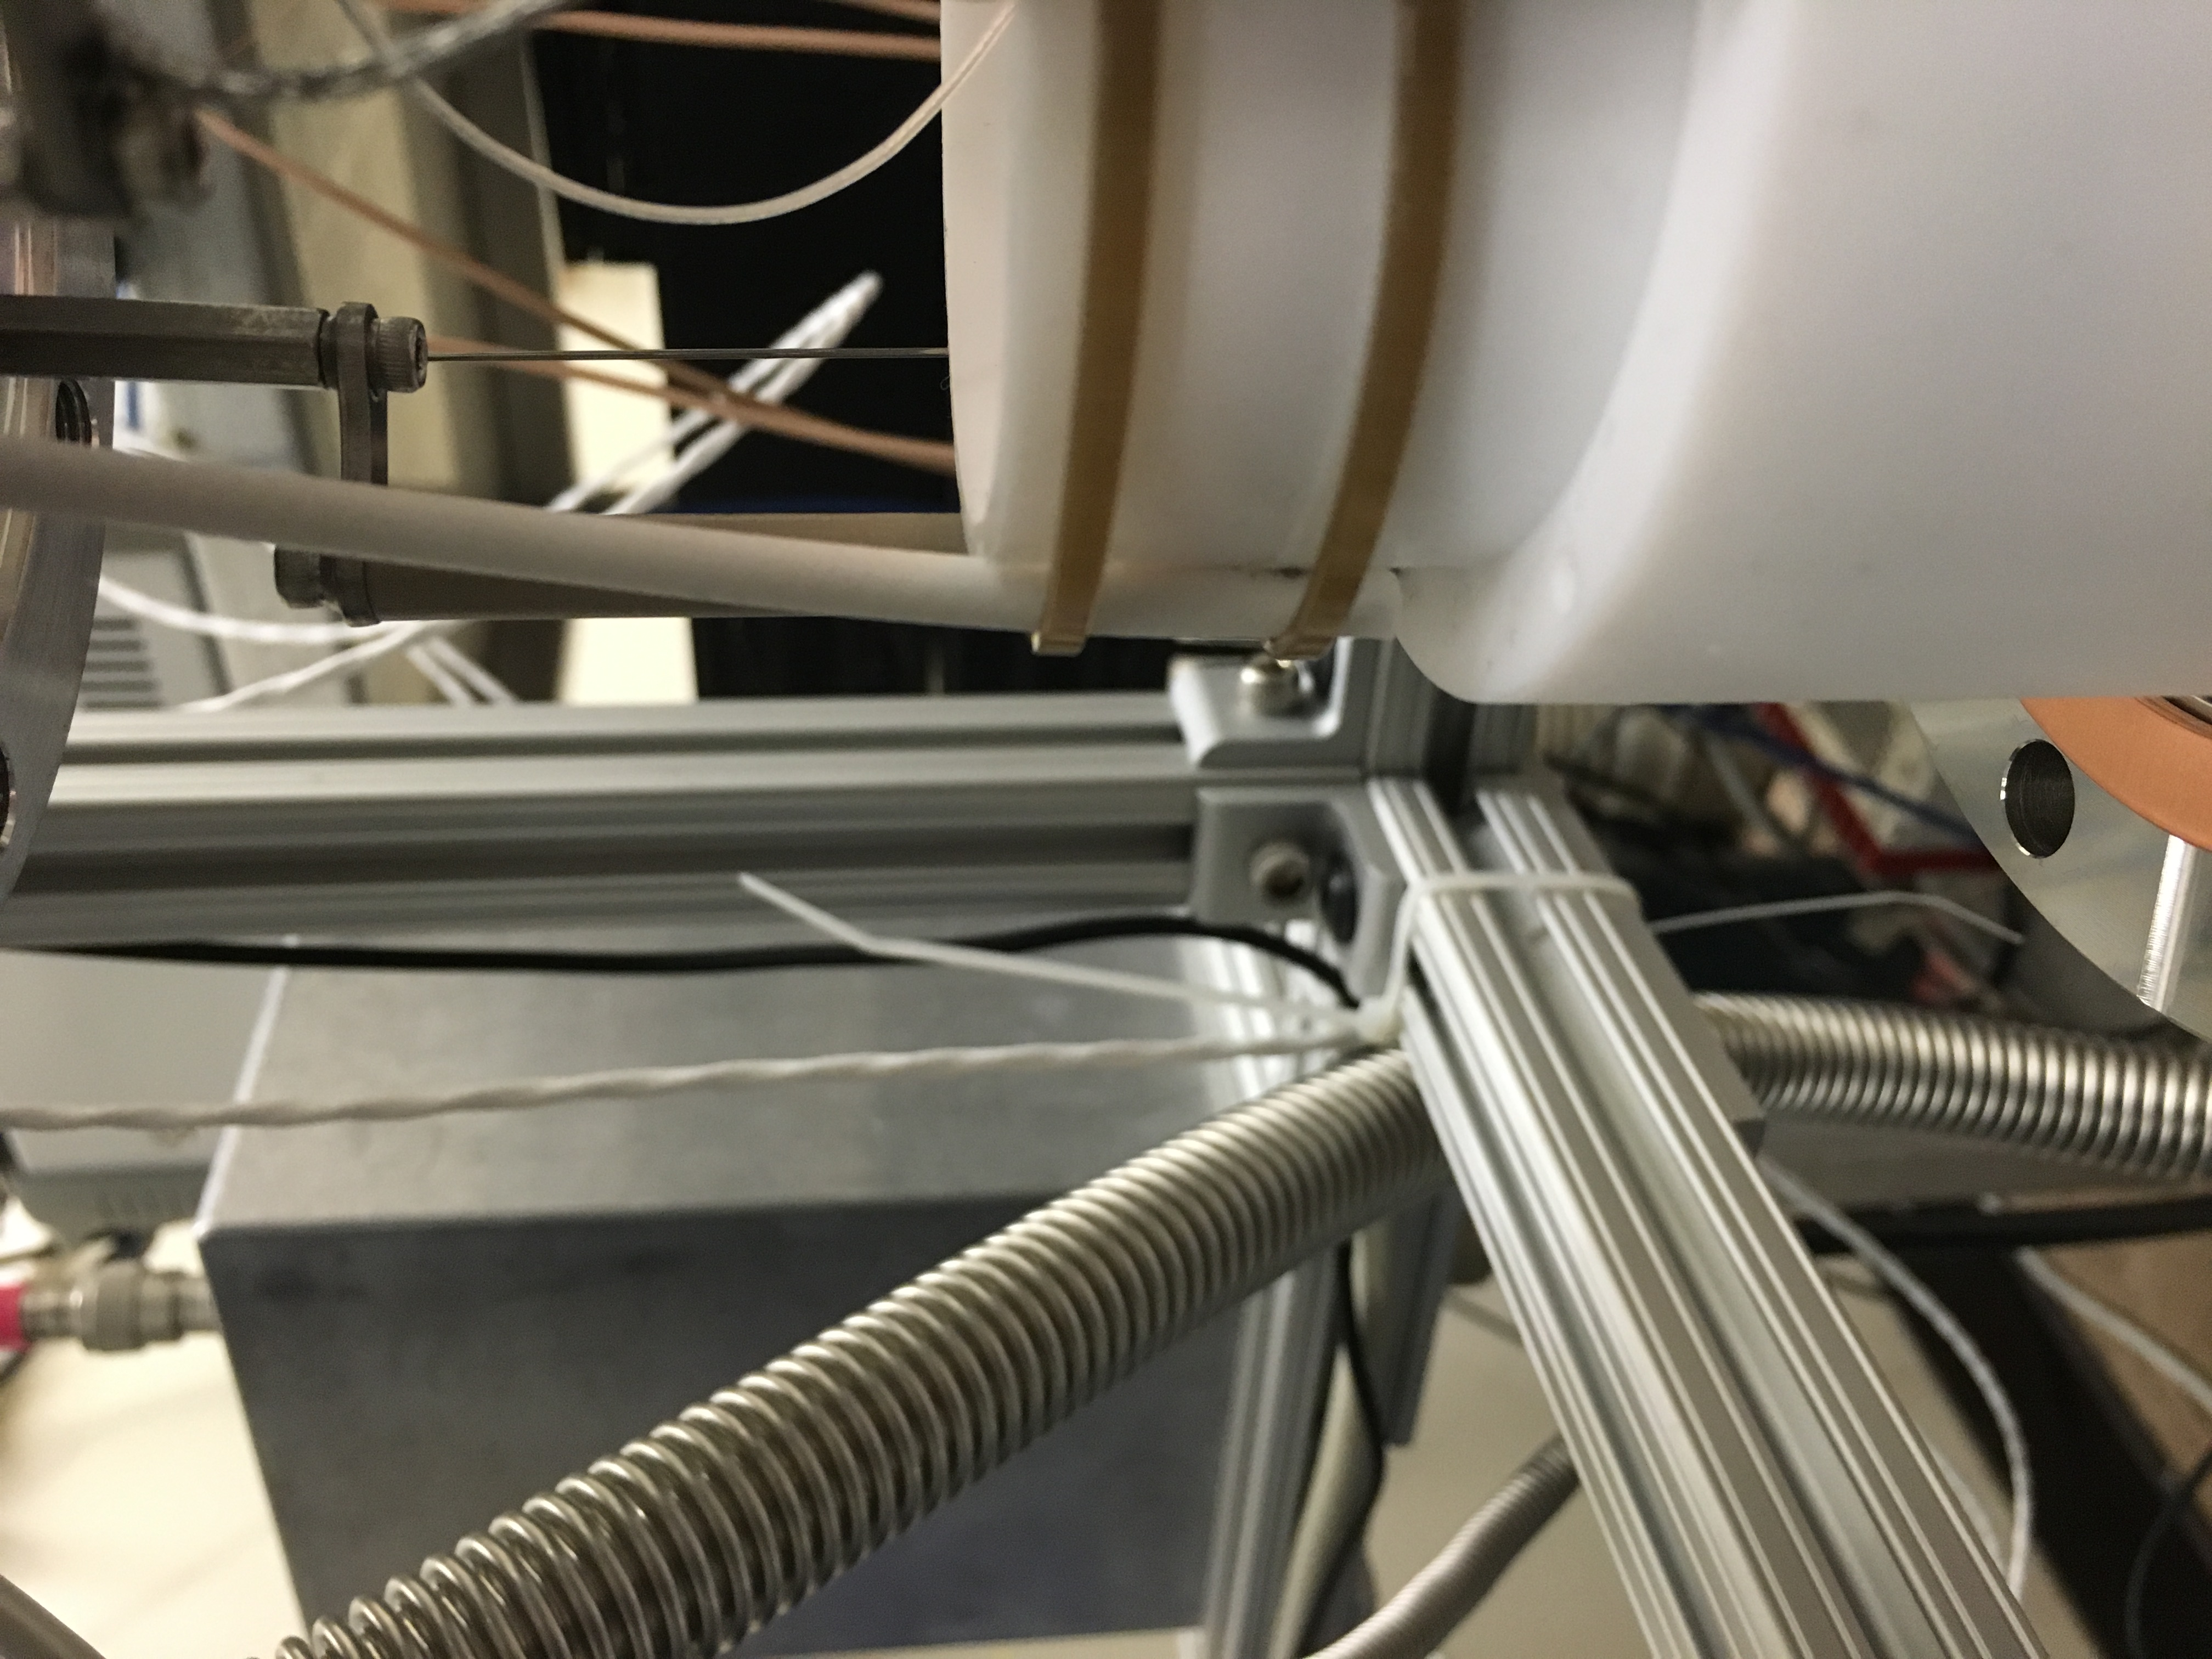
\includegraphics[width=3in, angle=-90]{figures/testbed/ft3_5.jpg}
\caption{Effect of holding the feed through in place with PEEK zip ties was explored, effects were minimal.}
\label{fig:aging}
\end{center}
\end{figure}


 
\subsubsection{Feedthrough Aging}
It was noticed during subsequent operation that the SHV-20 feed through was subject to some sort of aging process (black line in Figure~\ref{fig:aging}). A month of use resulted in noticeably lower voltage capabilities. The issue could have been any point along the entire voltage chain: feed through - custom cap - connection to cable - cable - connection to grid - grid. Tests focusing on different parts of the voltage chain didn't reveal any weak points. Instead, it was found that the SHV-20 feed though, itself, was subject to aging (red line in Figure~\ref{fig:aging}). 


\begin{figure}[htbp]
\begin{center}
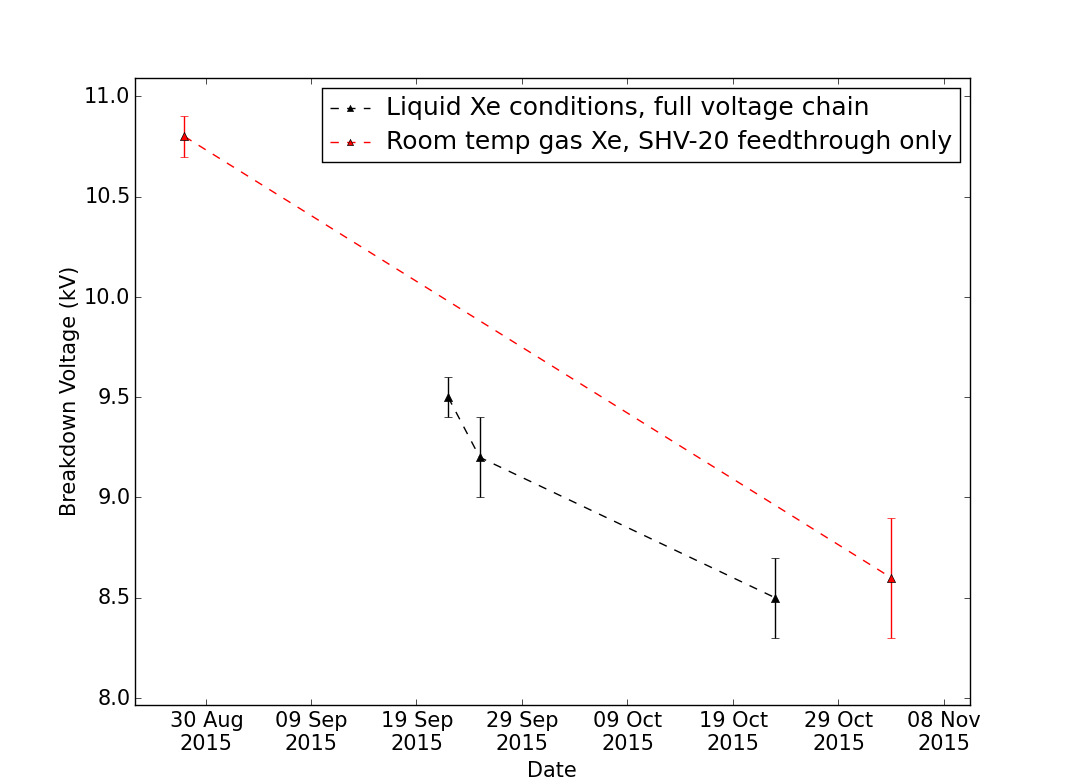
\includegraphics[width=5in]{figures/testbed/shv20_breakdowns.png}
\caption{The black line shows the aging observed in the course of normal operations. The red line shows breakdown tests of the SHV-20 feed though in gas, illustrating that the aging observed during operation was due to aging of the feed though.}
\label{fig:aging}
\end{center}
\end{figure}

Feedthrough aging can be the result of arcing and discharges which cause local heating and carbonization of an insulator surface. Once there is a carbon path, the insulator is considered "tracked" and then holds a much lower voltage than before.  Sophisticated \ac{HV} systems keep peak currents and fault energies to a minimum using series resistors. In this way, a breakdown event does not degrade system performance in the future. In addition to carbon tracks, there can also be insulator degradation from exposure to UV if there is ionization in the region. Xenon ionization is in the UV region of the spectrum, and so any ionization near a feed though insulator may degrade the feed through performance. In the case of this particular feed though, the high field which caused the breakdowns or ionization was likely a result of poor triple-point geometry. 


\subsection{Custom Feedthroughs}
To achieve better voltage performance, we moved away from typical feedthroughs composed of ceramic and metal. Figure~\ref{fig:ft4} shows a feed through made with a Swagelock reducing union. This blue and white PTFE piece connects 1/4~in \ac{SS} pipe to an 1/8~in PTFE tube, which then houses a \ac{SS} rod. The rod is screwed onto a connector, which holds a wire to connect to the grid. This feed through had stable voltage performance, but could not achieve sustained voltages higher than about 9~kV. A woven \ac{SS} shield was added to the feed though to reach higher voltages (Figure~\ref{fig:ft4} (left)) but this actually decreased the voltage performance to a maximum of about 5~kV.   

\begin{figure}[htbp]
\begin{center}
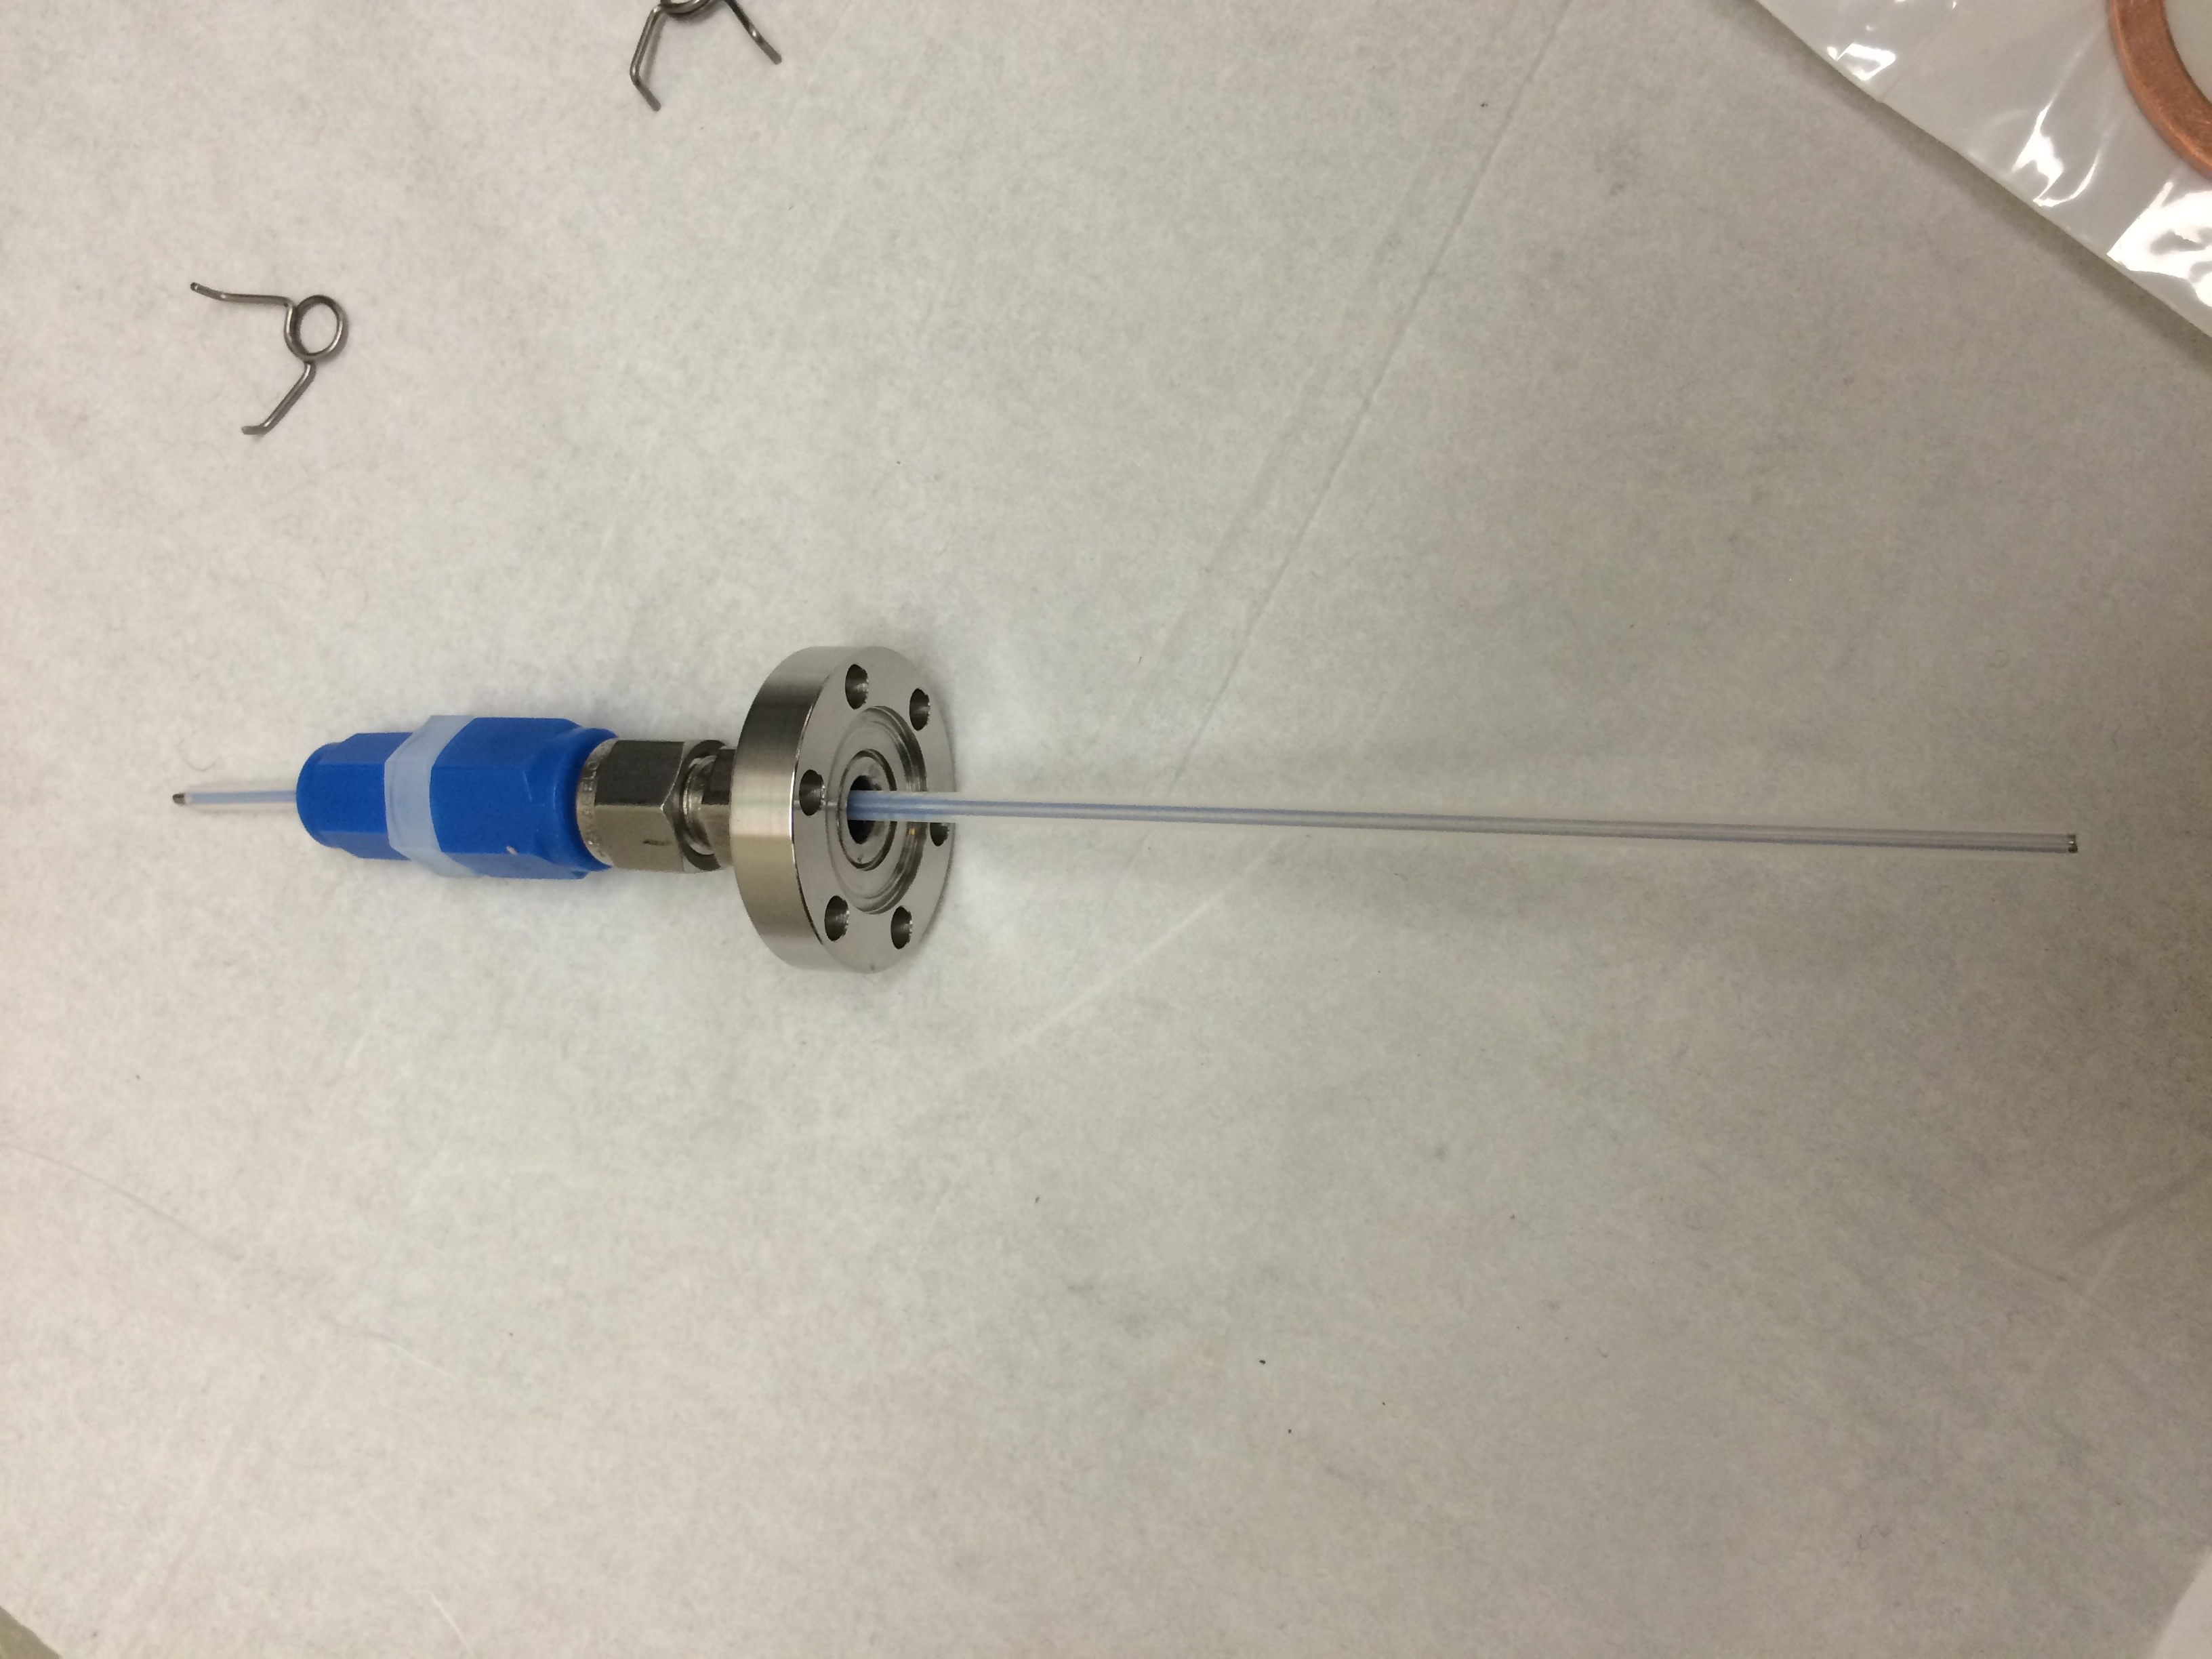
\includegraphics[width=0.3\textwidth, angle=-90]{figures/testbed/ft4_1.jpg}
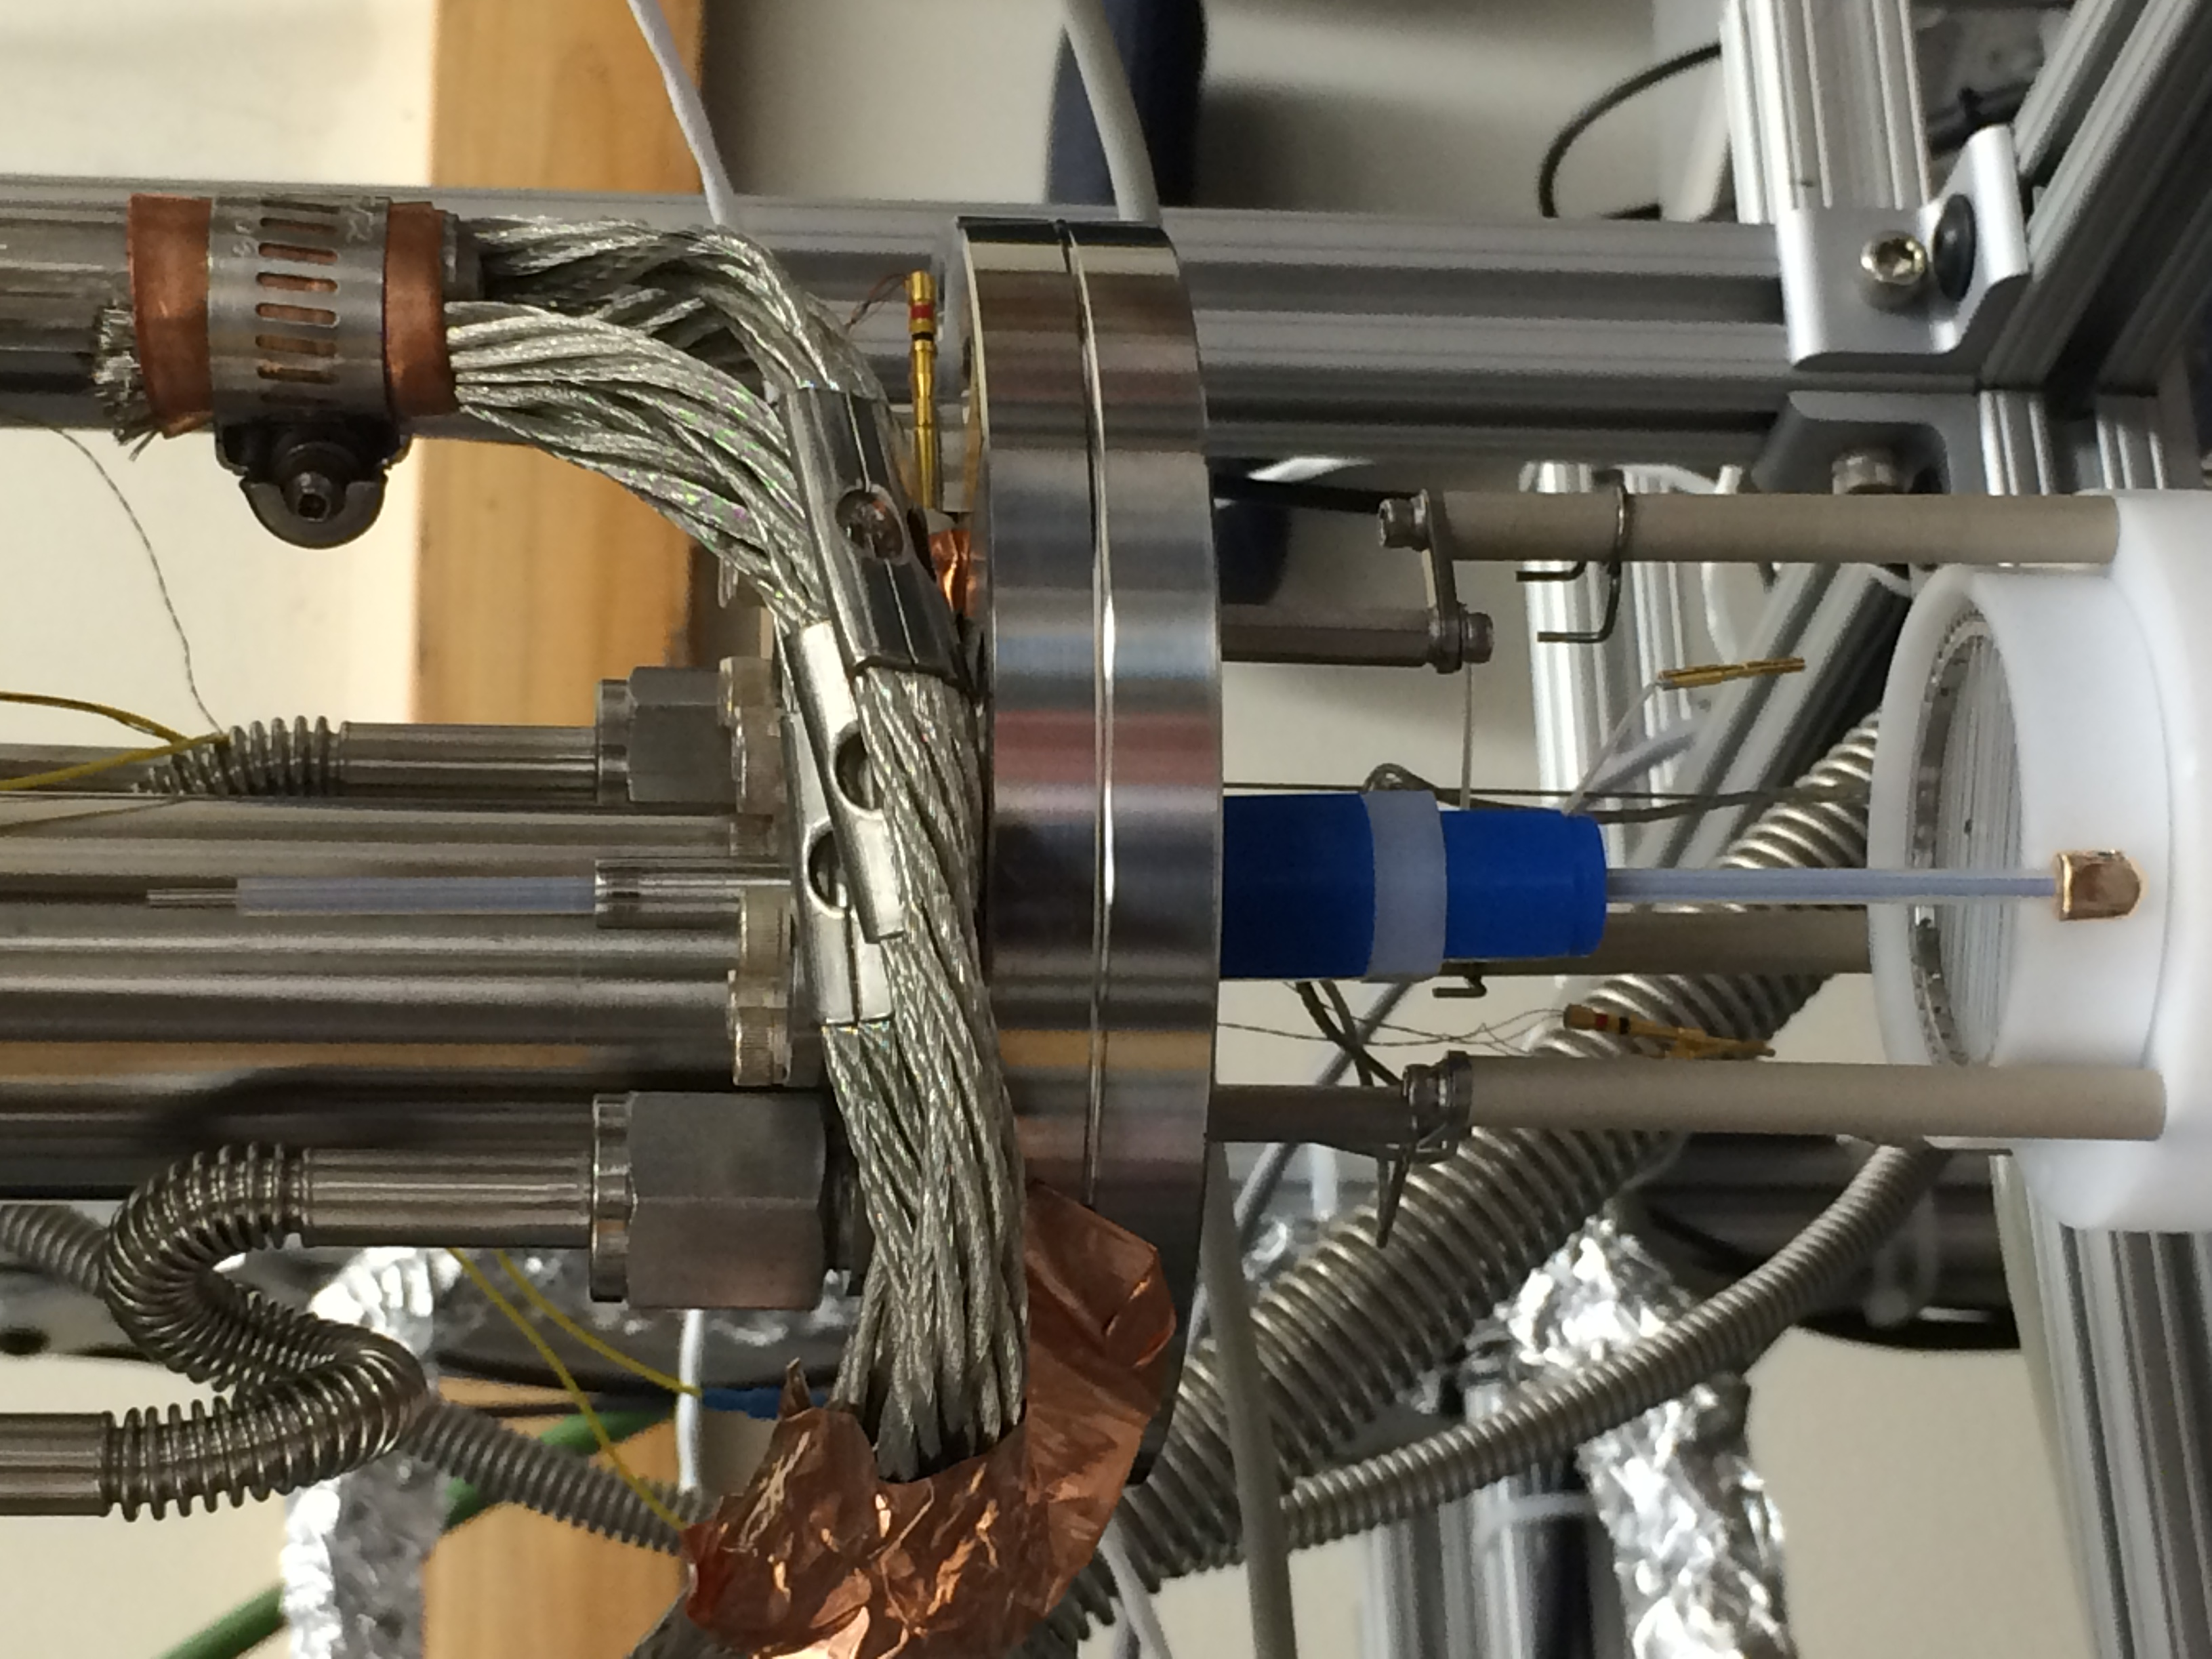
\includegraphics[width=0.3\textwidth, angle=-90]{figures/testbed/ft4_2.jpg}
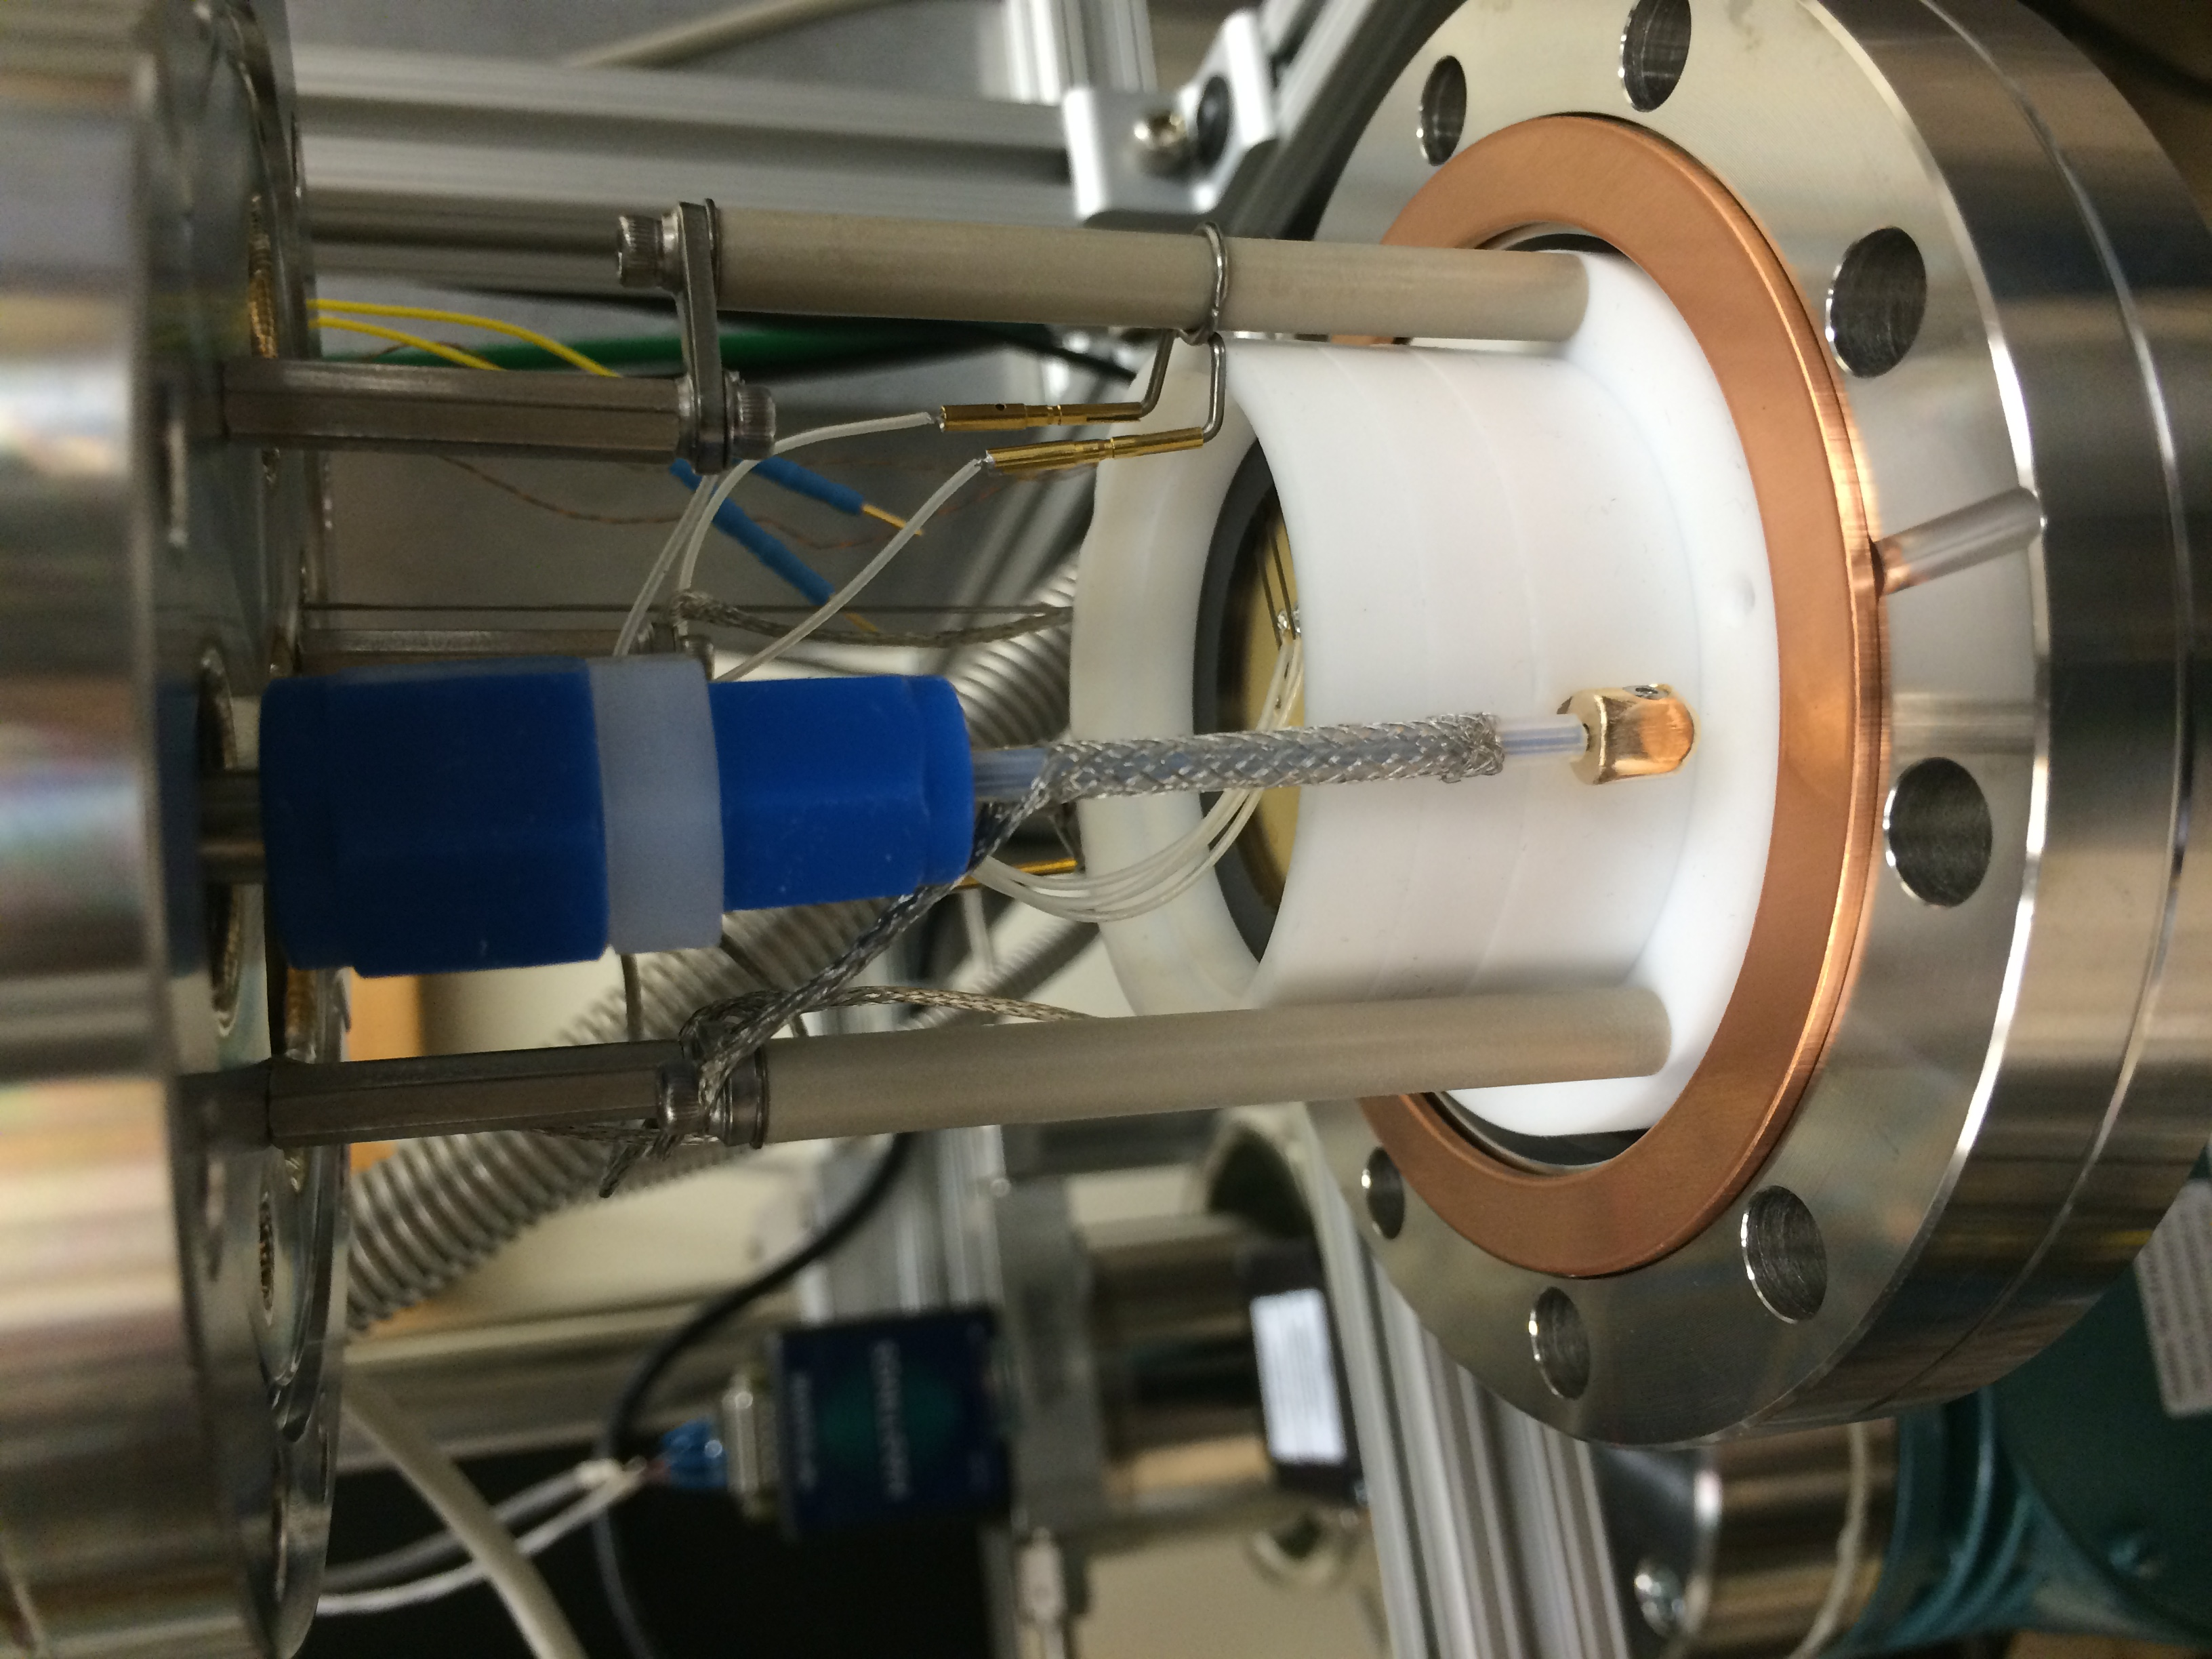
\includegraphics[width=0.3\textwidth, angle=-90]{figures/testbed/ft4_3.jpg}

\caption{First attempt at a custom feed through built out of Swagelock parts combined with basic materials like PTFE and stainless steel rods. The orientation shown (left) was later inverted due to concerns of temperature stress and pressure stress on the PTFE ferrules. The feedthrough as assembled (center) was functional, but higher voltage capability was desired. The effect of adding a grounding braid (right) was found to decrease the voltage capability instead of increasing it.  }
\label{fig:ft4}
\end{center}
\end{figure}


There are two issues with the approach of adding a grounding braid in this method: (1) the braid is not tight to the dielectric, which introduces peak fields between the dielectric and the braid (Figure~\ref{fig:will_comsol}) (2) at the braid termination, a small effective radius creates an enhanced radial field through the  dielectric and an enhanced field along the cable dielectric facing the high voltage. Peak fields can occur in unexpected places, greatly decreasing the voltage capability of a feedthrough that seems, naively, robust. The breakdown field of xenon gas depends on a variety of factors such as temperature (i.e density), purity, electrode shape, etc. Peak fields arising in gas regions in or around \ac{HV} feedthroughs are sources of unwanted of light and in the worst case complete breakdown and eventual degredation of the feedthrough. 

\begin{figure}[htbp]
\begin{center}
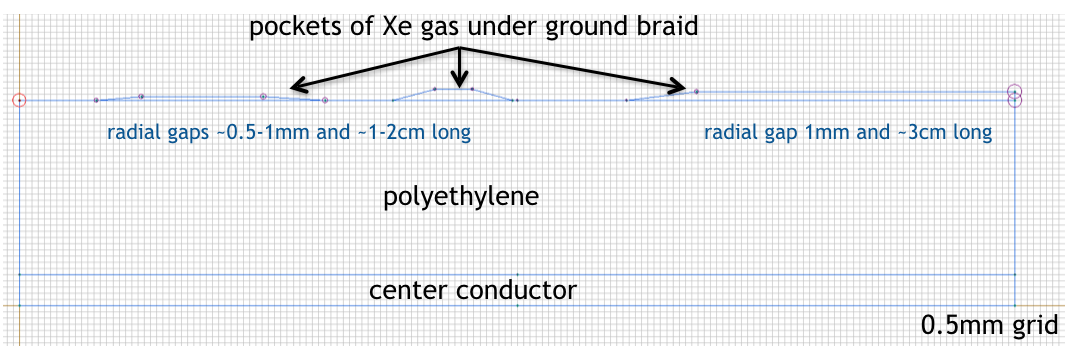
\includegraphics[width=\textwidth]{figures/testbed/will_comsol_1.png}\\
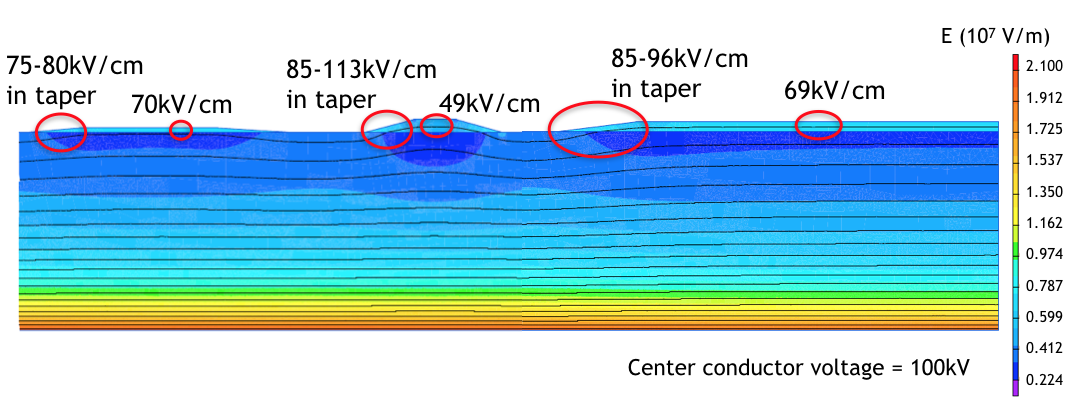
\includegraphics[width=\textwidth]{figures/testbed/will_comsol_2.png}

\caption{A COMSOL model by high voltage engineer W. Waldron showing that peak fields arise when gaps exist between dielectric and grounding braid.}
\label{fig:will_comsol}
\end{center}
\end{figure}



\begin{figure}[htbp]
\begin{minipage}{0.47\textwidth}
    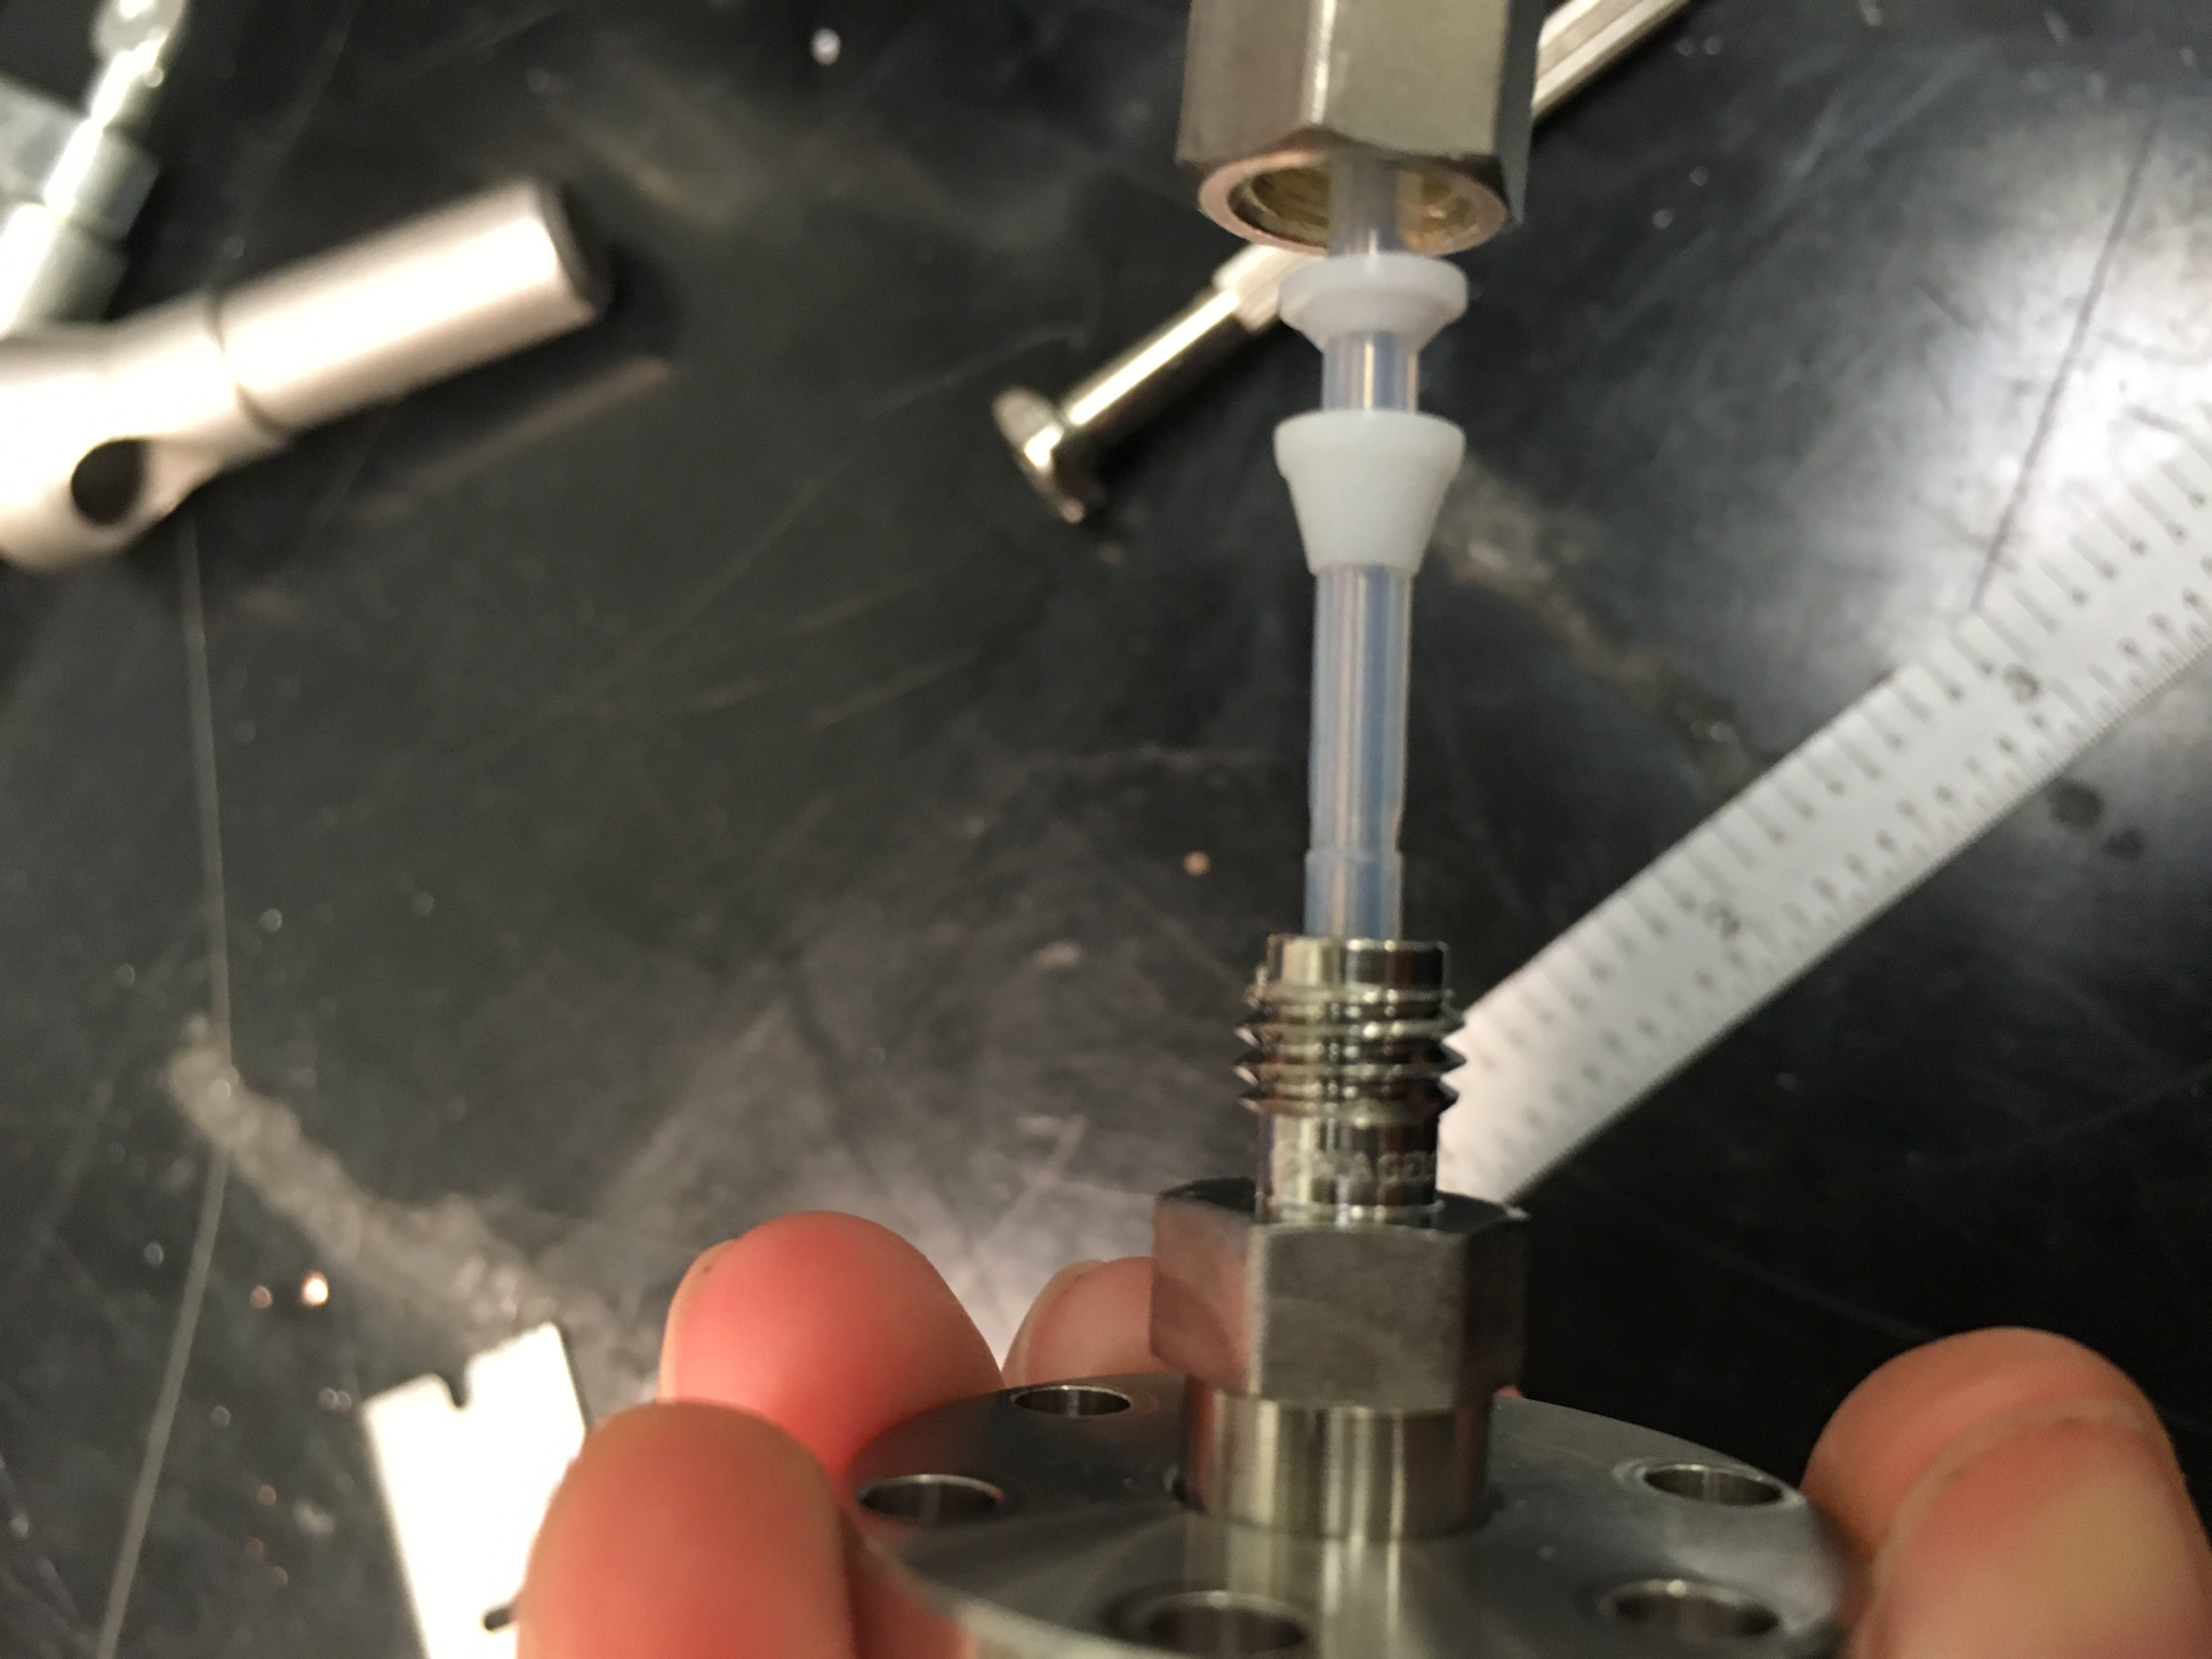
\includegraphics[width=\linewidth]{figures/testbed/ft5_1.jpg}
    \end{minipage}
    \hspace{\fill} % note: no blank line here
    \begin{minipage}{0.47\textwidth}
    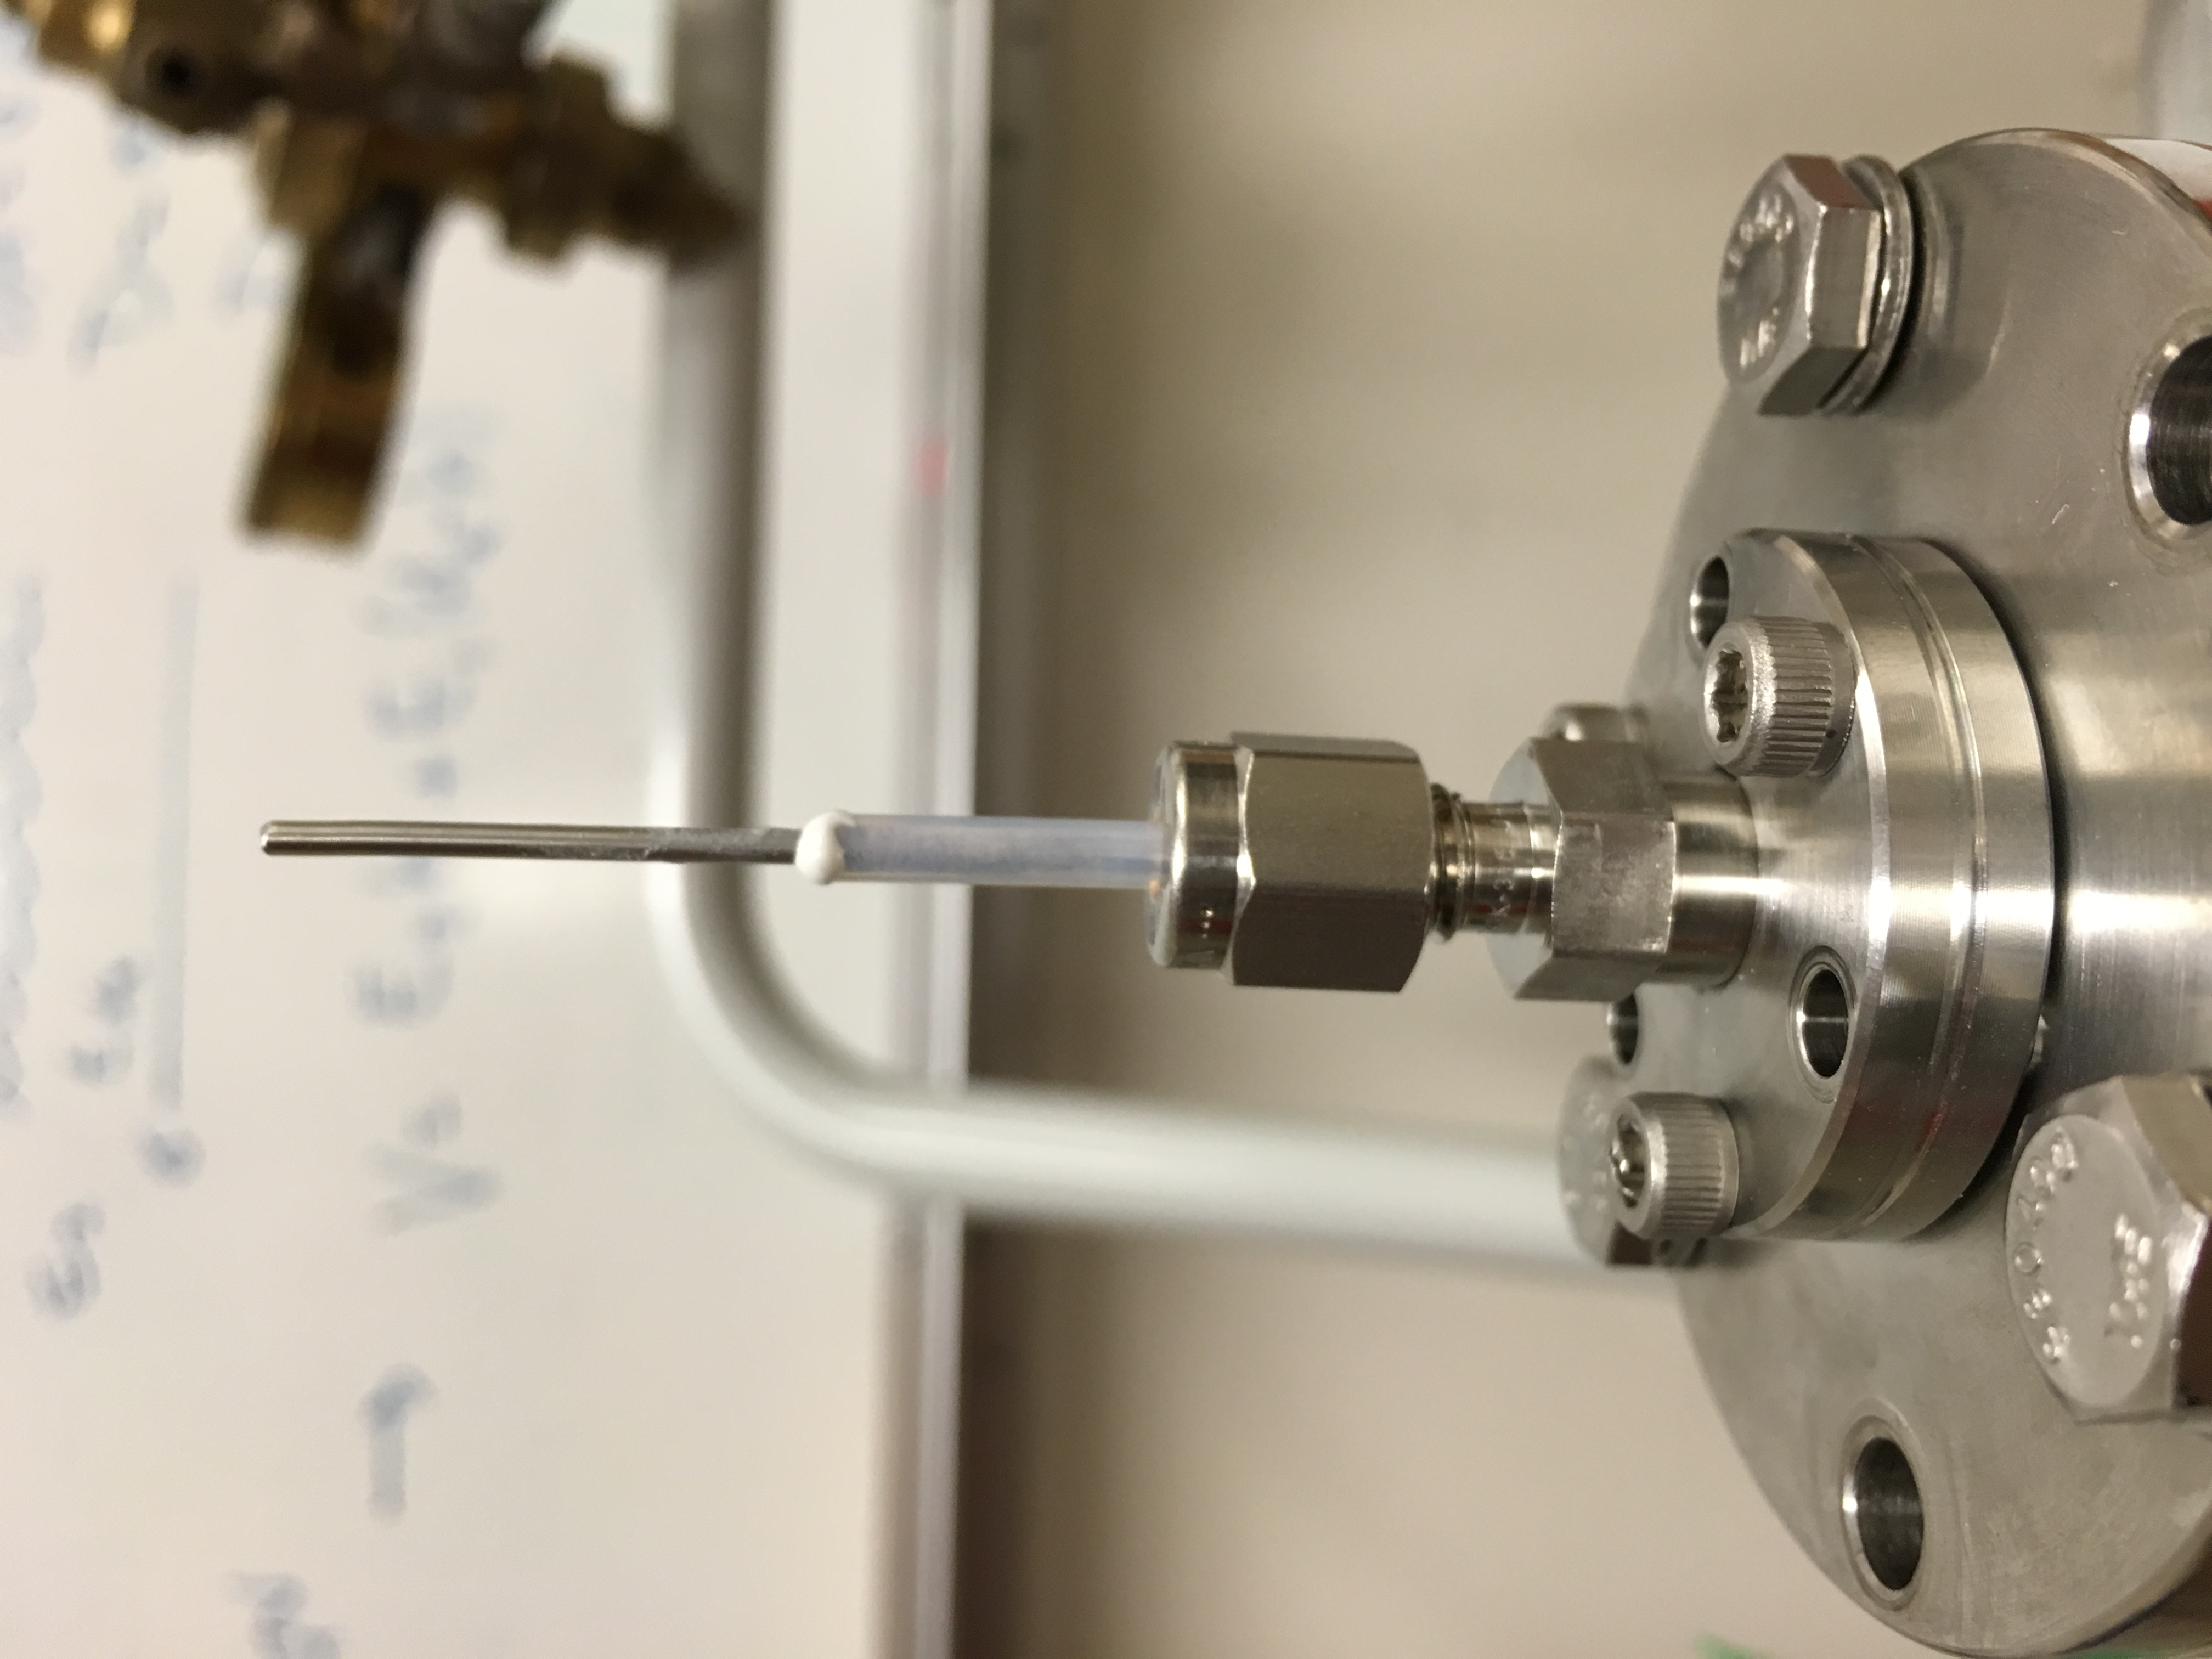
\includegraphics[width=\linewidth]{figures/testbed/ft5_2.jpg}
    \end{minipage}

    \vspace*{1cm} % vertical separation

    \begin{minipage}{0.47\textwidth}
    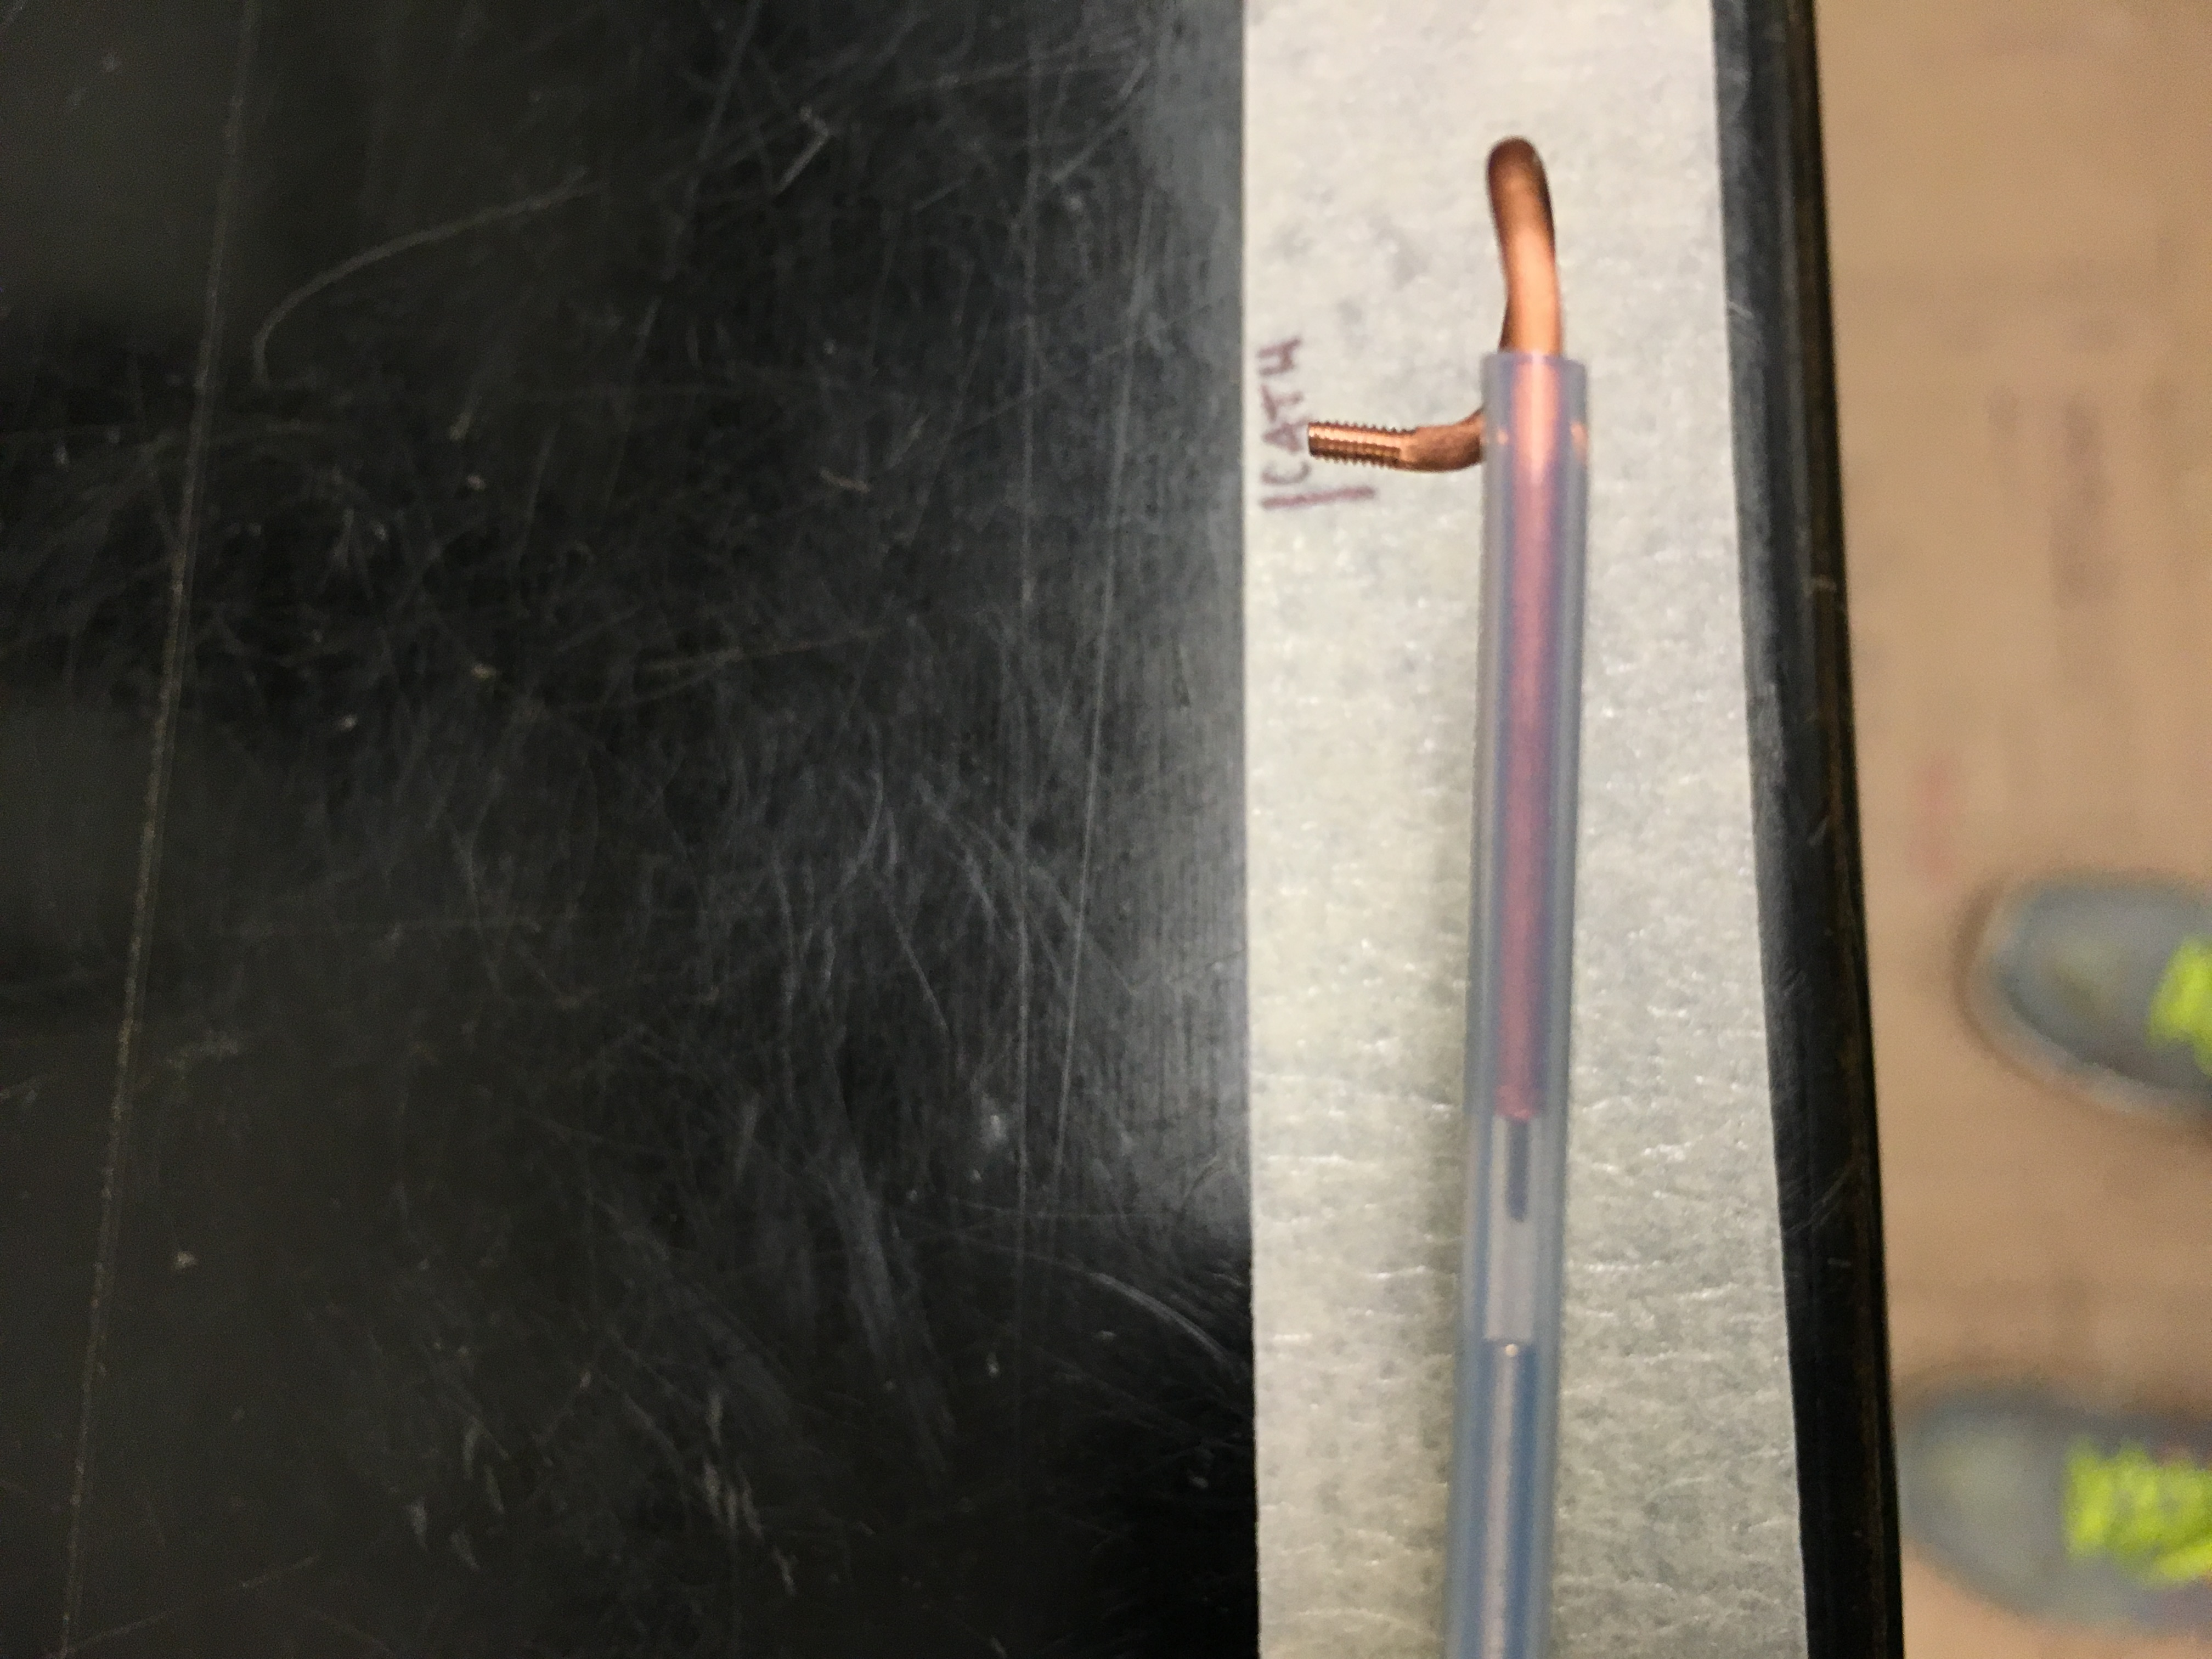
\includegraphics[width=\linewidth]{figures/testbed/ft5_3.jpg}
    \end{minipage}
    \hspace{\fill} % note: no blank line here
    \begin{minipage}{0.47\textwidth}
    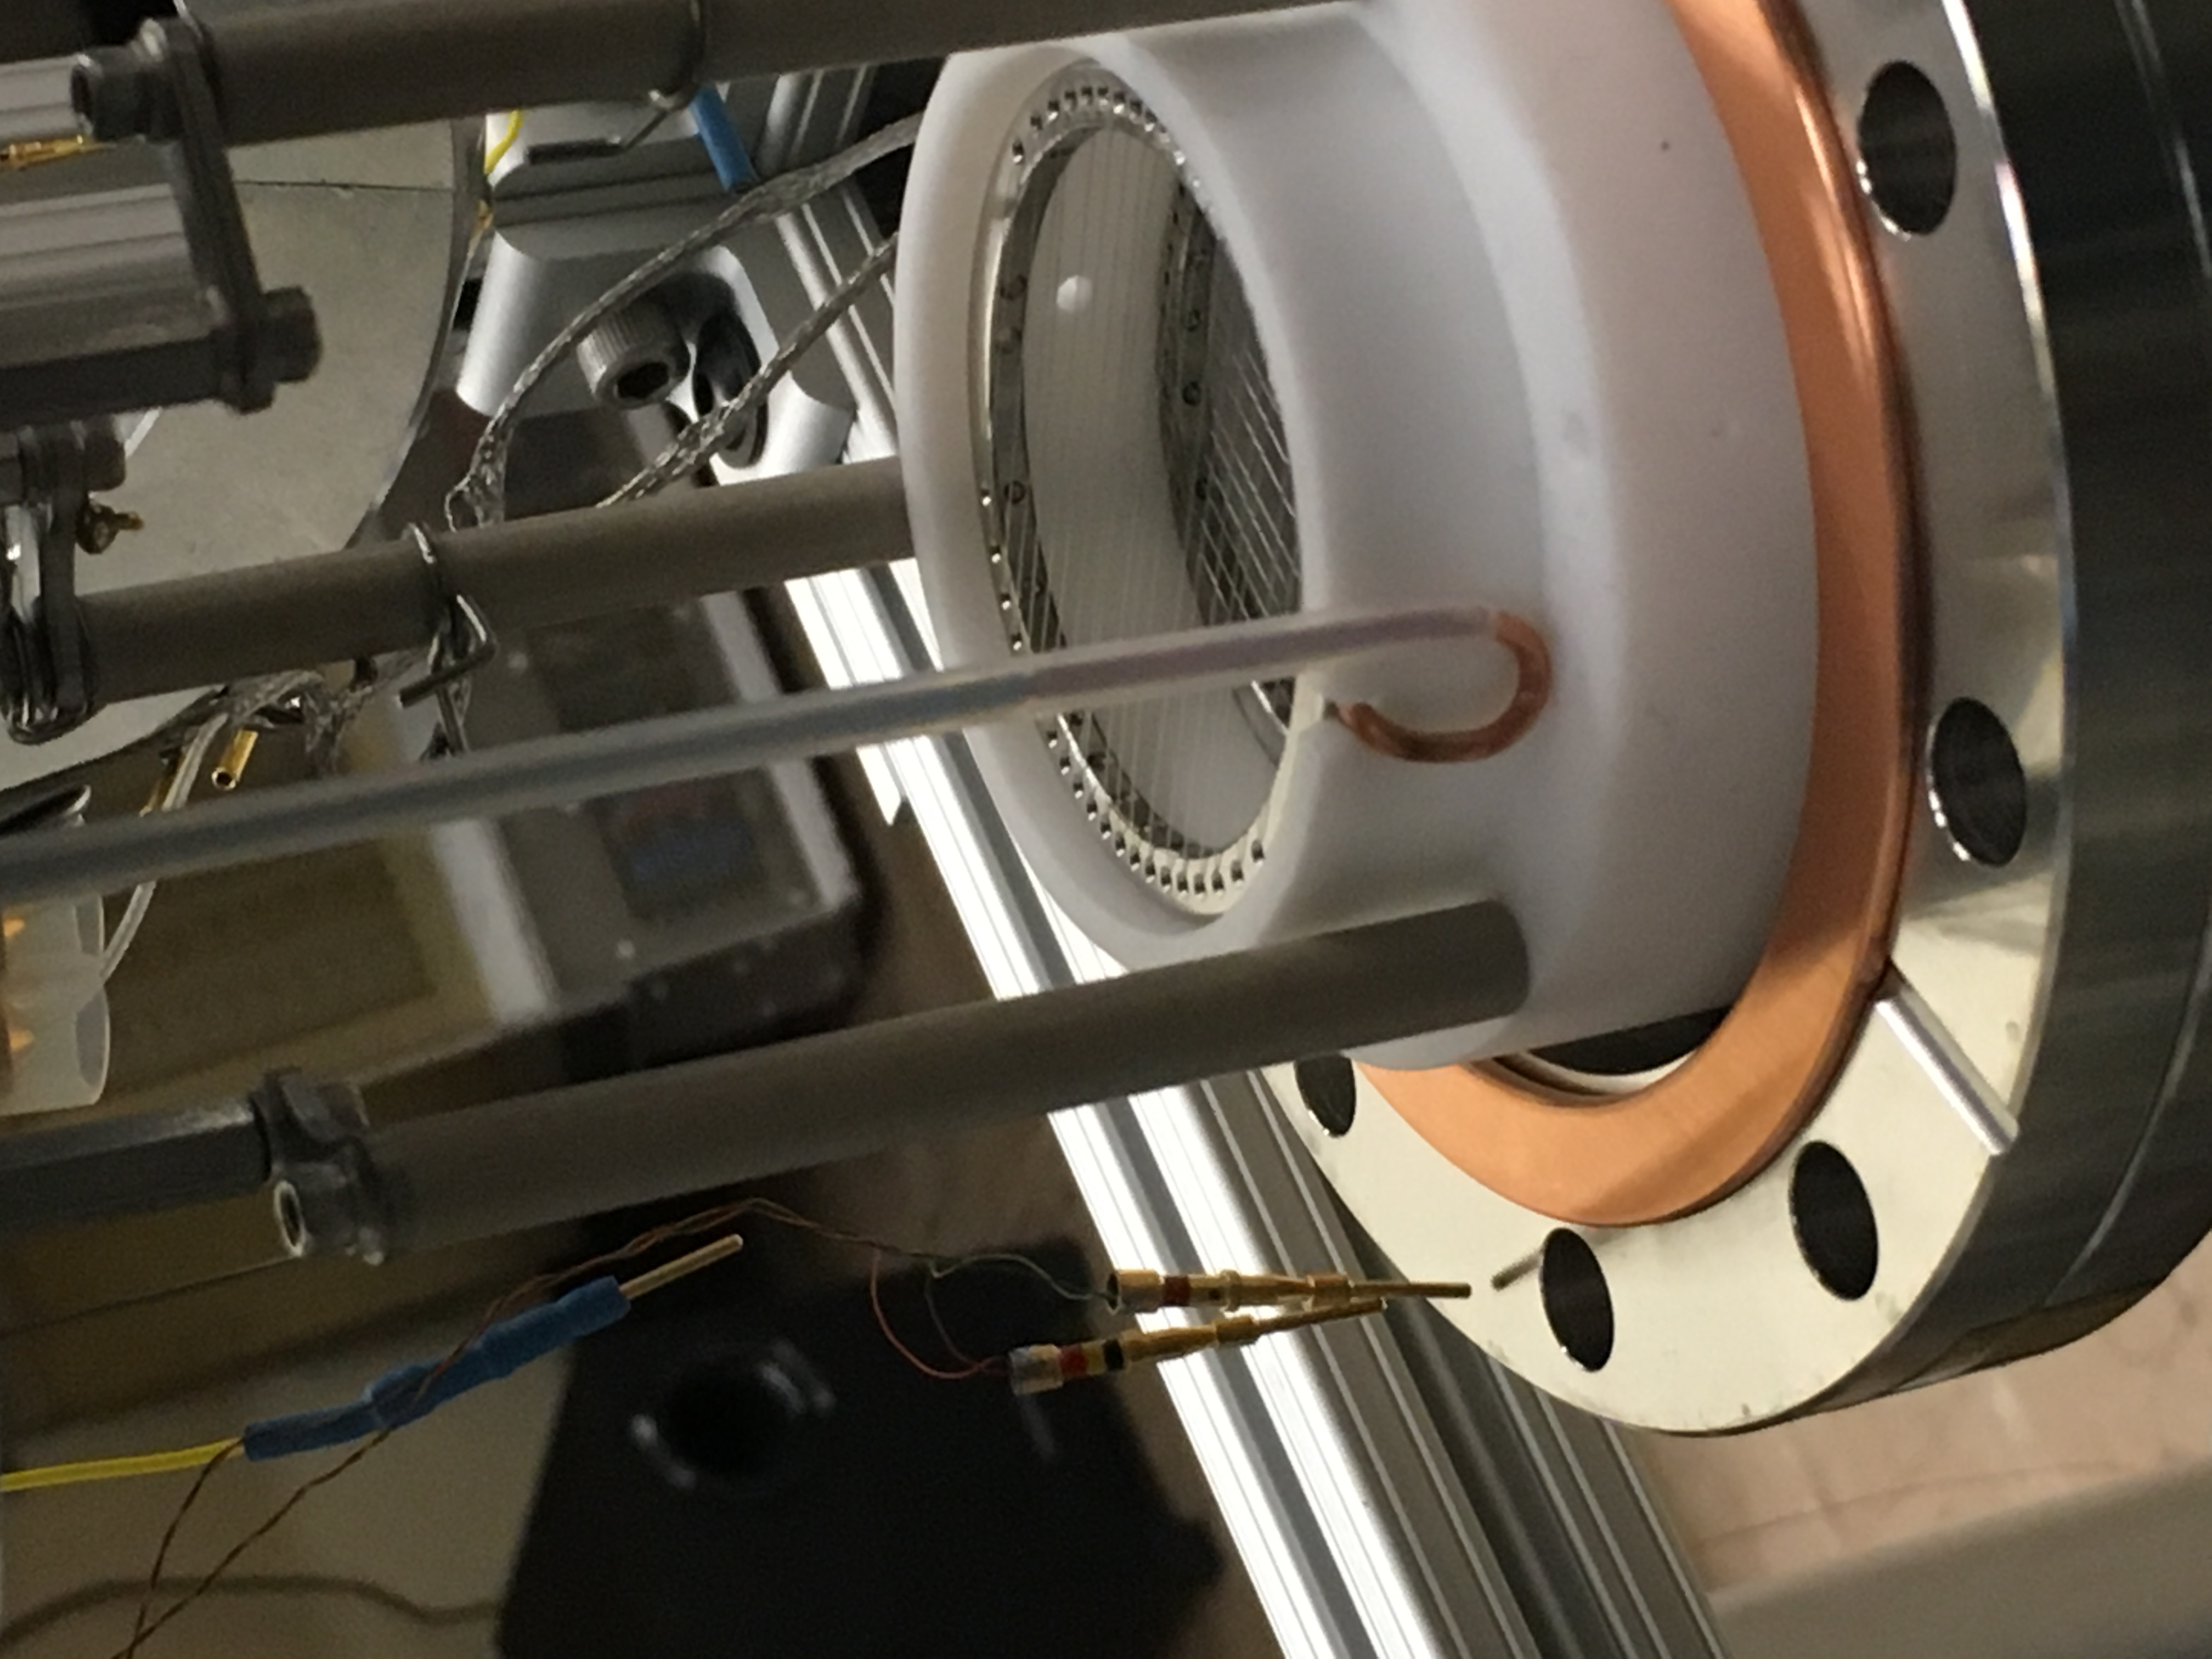
\includegraphics[width=\linewidth]{figures/testbed/ft5_4.jpg}
    \end{minipage}
\caption{Top: (left) (right) . Bottom: (left) (right).}
 \label{fig:shv20}
\end{figure}





%*****************************************
%*****************************************
%*****************************************
%*****************************************
%*****************************************
